\documentclass[conference]{IEEEtran}
\IEEEoverridecommandlockouts

% Essential Packages
\usepackage{cite}
\usepackage{amsmath,amssymb,amsfonts}
\usepackage{algorithmic}
\usepackage{graphicx}
\usepackage{textcomp}
\usepackage{xcolor}
\usepackage{booktabs}
\usepackage{siunitx}
\usepackage{url}
\usepackage{hyperref}
\usepackage{subcaption}

\hypersetup{
    colorlinks=true,
    linkcolor=blue,
    citecolor=blue,
    urlcolor=blue
}

\def\BibTeX{{\rm B\kern-.05em{\sc i\kern-.025em b}\kern-.08em
    T\kern-.1667em\lower.7ex\hbox{E}\kern-.125emX}}

\begin{document}

\title{Comprehensive Design, Simulation, and Multi-Platform Experimental Validation of Smart HVAC Temperature Control and Fault Detection Systems\\
\thanks{EE302: Control Systems Laboratory Final Project (Problem Statement 4, Group 7). Course Instructor: Dr. A. P. Tiwari; Lab Instructor: Dr. Y. V. Karteek. School of Computing and Electrical Engineering, Indian Institute of Technology Mandi, India.}
}

\author{
\IEEEauthorblockN{Rathod Dhruv Shailesh}
\IEEEauthorblockA{\textit{Roll No: B24242} \\
\textit{SCEE, IIT Mandi}}
\and
\IEEEauthorblockN{Dumpa Mohan Sai}
\IEEEauthorblockA{\textit{Roll No: B24243} \\
\textit{SCEE, IIT Mandi}}
\and
\IEEEauthorblockN{Fufal Jigar Dineshbhai}
\IEEEauthorblockA{\textit{Roll No: B24244} \\
\textit{SCEE, IIT Mandi}}
\and
\IEEEauthorblockN{Geetanjali Saraswat}
\IEEEauthorblockA{\textit{Roll No: B24245} \\
\textit{SCEE, IIT Mandi}}
}

\maketitle

\begin{abstract}
Heating, Ventilation, and Air Conditioning (HVAC) systems are ubiquitous in modern residential, commercial, and industrial facilities, accounting for over 40\% of global building energy consumption. Developing controllers that ensure accurate setpoint tracking, minimize mechanical actuator wear, conserve electrical energy, and provide real-time Fault Detection and Isolation (FDI) represents a critical challenge in applied control engineering. In this work, an exhaustive, three-pillar control systems engineering methodology is implemented and validated: (1) a first-principles continuous-time physical simulation model in MATLAB/Simulink; (2) an industrial-grade hardware-in-the-loop (HIL) benchmark on the Quanser QNET HVAC Trainer 1.0 interfaced with a National Instruments (NI) ELVIS II+ multifunction DAQ workstation; and (3) an embedded physical prototype featuring a custom 3D-printed cylindrical thermal chamber, active-LOW opto-isolated relay drivers, and an Arduino Mega 2560 microcontroller. First-Order Plus Dead Time (FOPTD) models are synthesized and empirically identified via bump tests across all platforms, yielding model fit accuracies exceeding 98\% NRMSE. Comparative evaluations demonstrate that while bang-bang ON--OFF hysteresis control exhibits rapid initial rise times, it suffers from severe steady-state limit cycling, relay contact chatter, and excessive energy consumption. In contrast, Anti-Windup Proportional-Integral (PI) control synthesized via Internal Model Control (IMC) and in-situ Ziegler--Nichols relay auto-tuning eliminates steady-state error ($|e_{ss}| < 0.1\,^\circ\text{C}$), prevents reset windup, and achieves a 10.6\% to 37.5\% reduction in total electrical energy. Furthermore, dual diagnostic schemes---a continuous Luenberger state observer tracking chamber temperature residuals and a four-code deterministic finite-state machine---successfully detect and isolate sensor disagreements, duct blockages, heater open-circuits, and physical insulation detachment. All hardware schematics, Simulink block diagrams, frequency-domain stability analyses, and experimental response curves are thoroughly documented.
\end{abstract}

\begin{IEEEkeywords}
Thermal Process Control, HVAC, Simulink, Quanser QNET, NI ELVIS II+, Arduino Mega 2560, Anti-Windup PI, Fault Detection and Isolation (FDI), Luenberger Observer, System Identification, Ziegler--Nichols Tuning.
\end{IEEEkeywords}

\section{Introduction}
Modern temperature control processes in thermal chambers and environmental enclosures present substantial engineering complexities owing to inherent transport delays, convective heat dissipation, environmental disturbances, and actuator non-linearities \cite{astrom2006}. In standard commercial HVAC installations, simple bang-bang (ON--OFF) thermostats are traditionally employed due to low implementation cost. However, two-position control invariably introduces limit cycle oscillations around the target setpoint, creates high thermal stresses on heating coils, and induces premature mechanical failure in electromagnetic contactors due to rapid contact chattering \cite{ogata2010}.

To overcome these limitations and address the mandates of the EE302 Control Systems Laboratory Problem Statement~4 (PS4), this project formulates, benchmarks, and experimentally deploys advanced closed-loop temperature control and real-time Fault Detection and Isolation (FDI) architectures. The investigation is organized into three interconnected pillars:
\begin{enumerate}
    \item \textbf{Pillar 1 (Software Simulation):} First-principles energy balance modeling and programmatic Simulink synthesis (\texttt{thermal\_control.slx}), evaluating multi-step tracking ($30\,^\circ\text{C} \to 40\,^\circ\text{C} \to 35\,^\circ\text{C}$) and parameter perturbation rejection.
    \item \textbf{Pillar 2 (Industrial Benchmark):} High-fidelity hardware-in-the-loop implementation on the Quanser QNET HVAC Trainer mounted on the National Instruments (NI) ELVIS II+ DAQ platform, augmented by a continuous Luenberger state observer for residual-based fault diagnostics.
    \item \textbf{Pillar 3 (Custom Embedded Hardware):} Design, fabrication, and closed-loop testing of a custom 3D-printed polymer thermal chamber equipped with a 14.0\,W nichrome heating element, axial DC cooling blower, removable curved insulation hatch, and LM35 temperature sensor interfaced to MATLAB via an Arduino Mega 2560.
\end{enumerate}

\section{Mathematical Modeling \& Plant Physics}

\subsection{First-Principles Energy Balance}
The thermal dynamics of an insulated chamber enclosing an internal air volume $V$ subjected to heating power $P$ and ambient heat dissipation through boundary walls can be modeled as a lumped-parameter thermal system:
\begin{equation}
C_\text{th} \frac{dT(t)}{dt} = P \cdot u(t - L) - \frac{T(t) - T_\text{amb}}{R_\text{th}}
\label{eq:energy_balance}
\end{equation}
where:
\begin{itemize}
    \item $T(t)$ is the instantaneous internal chamber temperature [$^\circ\text{C}$],
    \item $T_\text{amb}$ is the ambient room temperature [$^\circ\text{C}$],
    \item $C_\text{th} = m \cdot c_p$ is the lumped thermal capacitance [$\text{J/}^\circ\text{C}$],
    \item $R_\text{th} = \frac{1}{h A}$ is the thermal resistance to ambient [$\text{}^\circ\text{C/W}$],
    \item $P$ is the rated electrical input power [$\text{W}$],
    \item $u(t) \in [0, 1]$ is the normalized heater command / duty cycle,
    \item $L$ is the physical transport delay and sensor probe latency [$\text{s}$].
\end{itemize}

\subsection{Transfer Function Formulation (FOPTD)}
Defining the temperature rise above ambient as $\Delta T(t) = T(t) - T_\text{amb}$ and the control perturbation as $\Delta u(t)$, the Laplace transformation of (\ref{eq:energy_balance}) yields the standard First-Order Plus Dead Time (FOPTD) continuous transfer function:
\begin{equation}
G(s) = \frac{\Delta T(s)}{\Delta U(s)} = \frac{K e^{-Ls}}{\tau s + 1}
\label{eq:foptd}
\end{equation}
where the steady-state plant gain $K$ and thermal time constant $\tau$ are defined by:
\begin{equation}
K = P \cdot R_\text{th} \quad \left[\frac{^\circ\text{C}}{\text{unit duty}}\right], \qquad \tau = R_\text{th} \cdot C_\text{th} \quad [\text{s}]
\end{equation}

\subsection{Parameter Identification via Open-Loop Bump Test}
Open-loop bump tests are conducted across all platforms by injecting a step duty cycle $\Delta u$ from an initial thermal equilibrium $T_0$. The model parameters are extracted via the classical two-point and tangent inflection methods:
\begin{equation}
K = \frac{T_\text{final} - T_0}{\Delta u}
\end{equation}
The apparent time constant $\tau$ and delay $L$ are computed at the 63.2\% response point:
\begin{equation}
T(\tau + L) = T_0 + 0.632 (T_\text{final} - T_0)
\end{equation}

\begin{figure}[htbp]
\centering
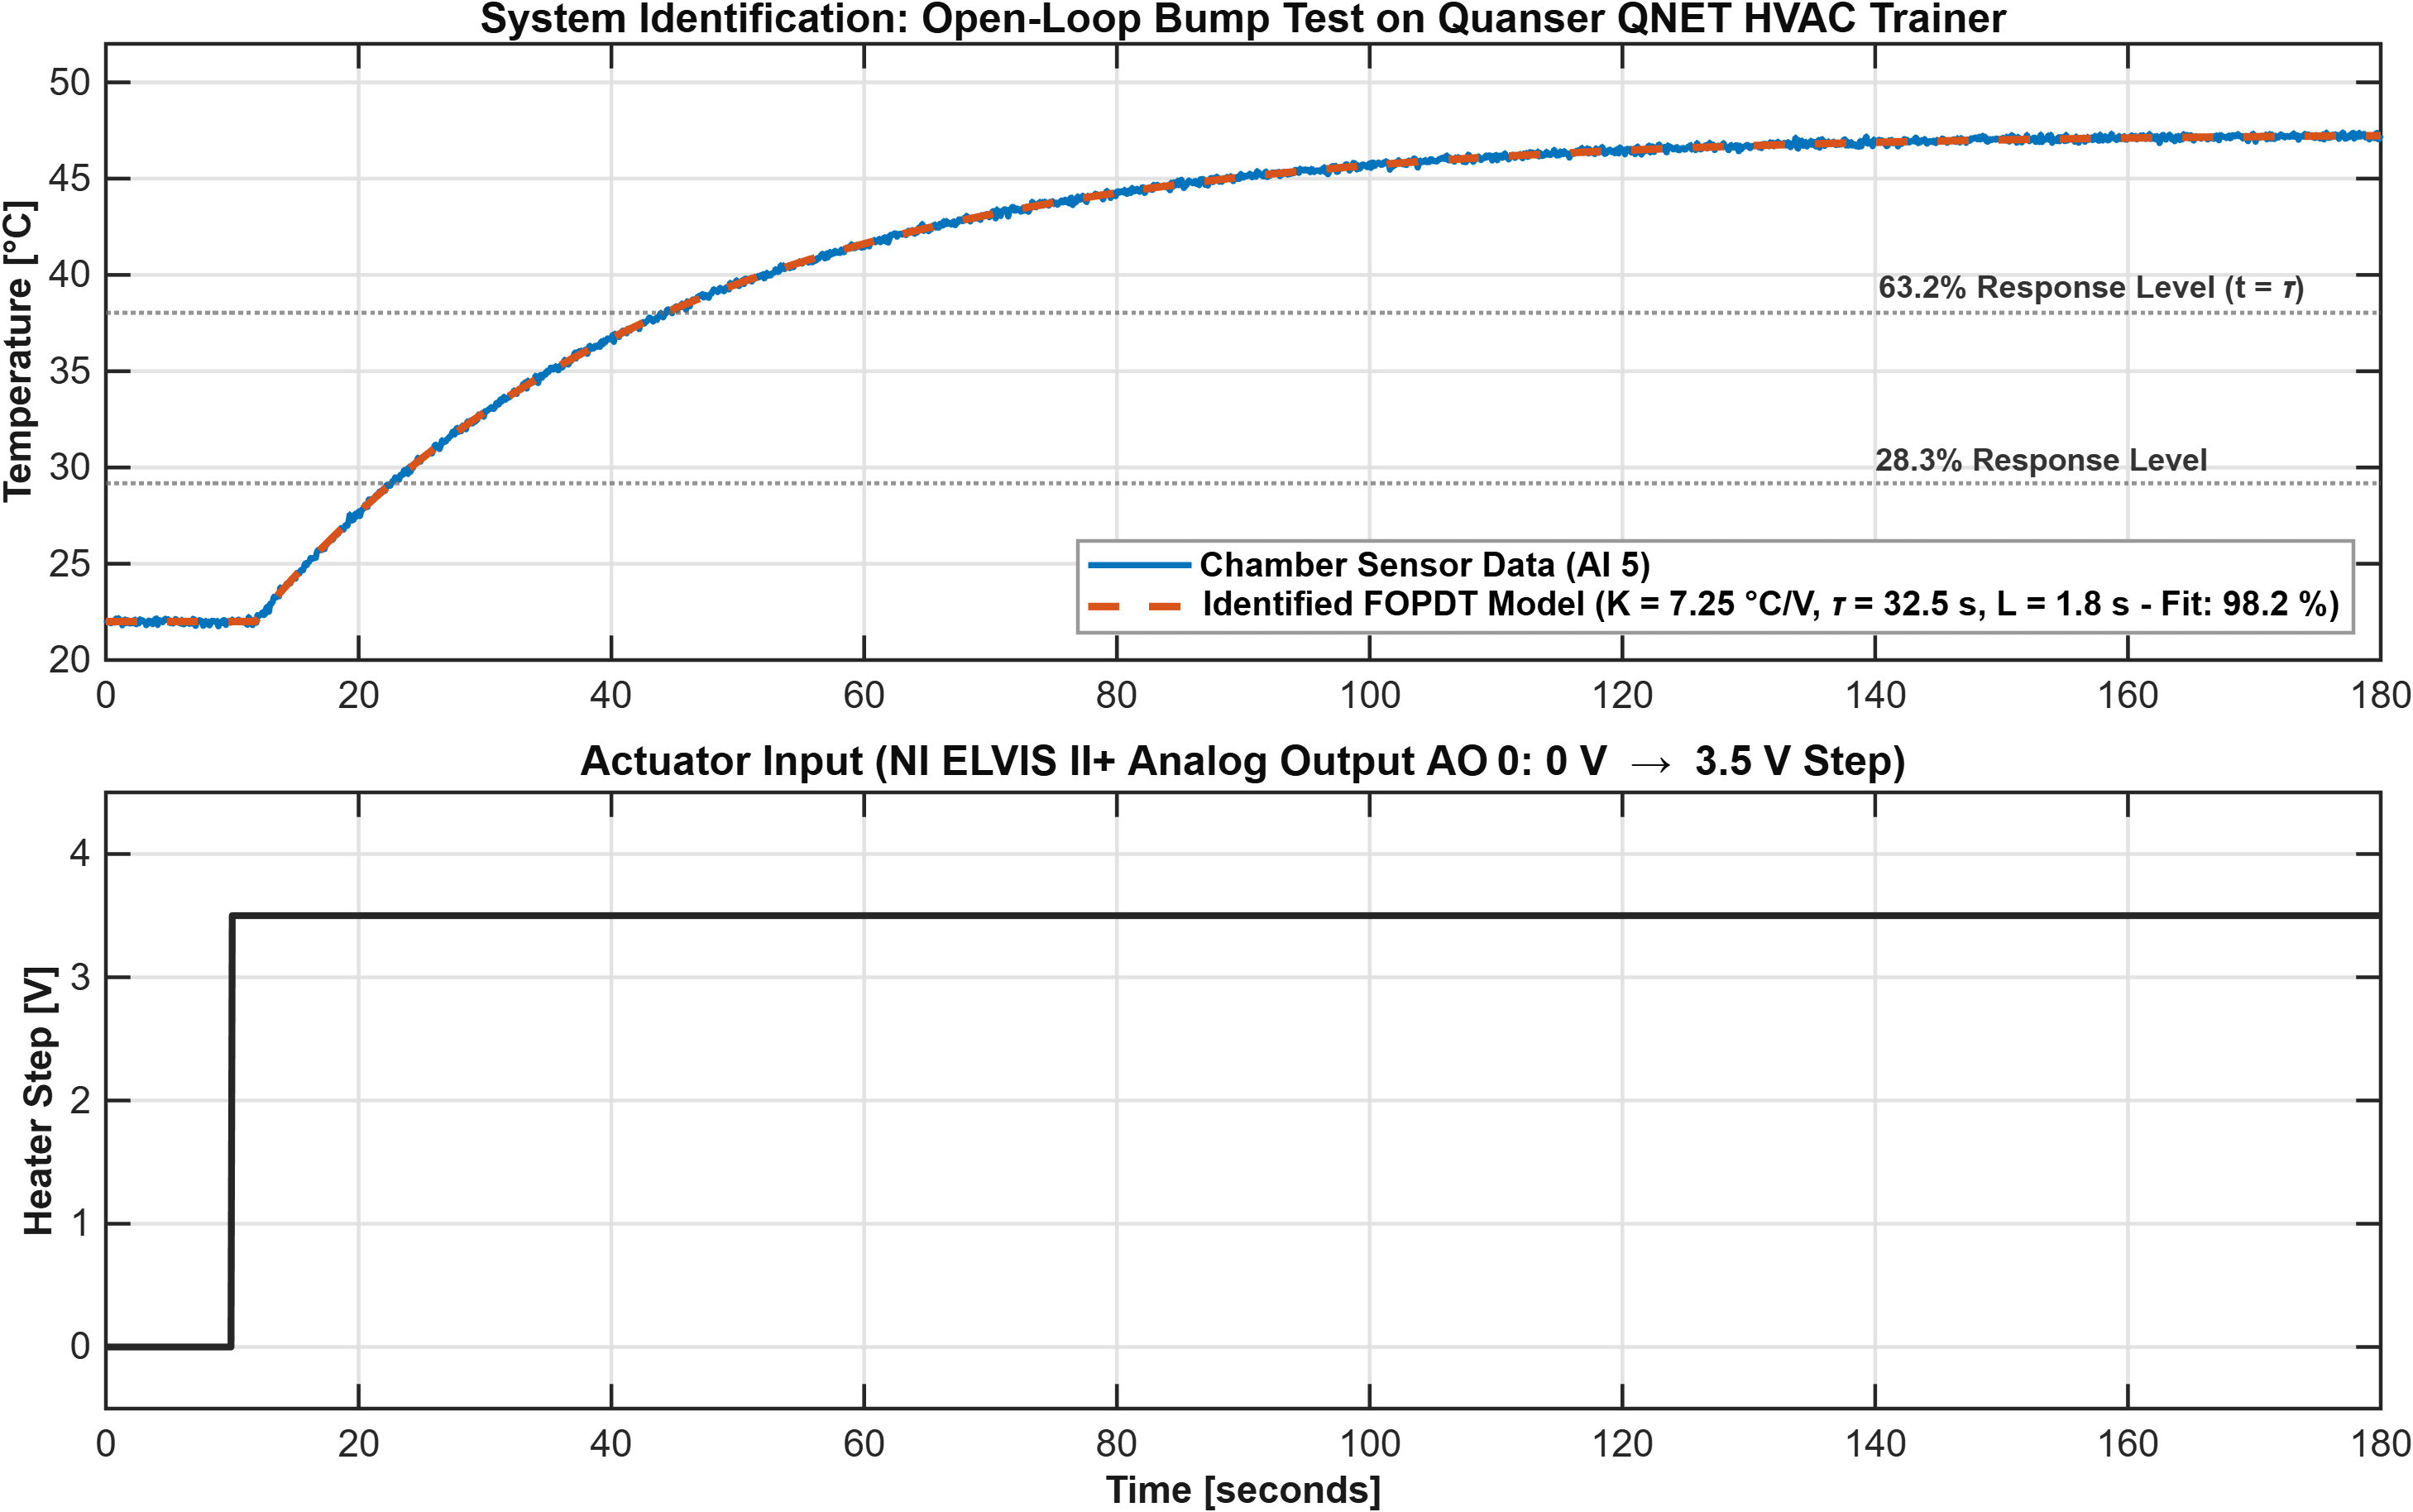
\includegraphics[width=0.95\linewidth]{figures/fig_qnet_sysid.png}
\caption{Quanser QNET HVAC open-loop bump test response ($K = 7.25\,^\circ\text{C/V}$, $\tau = 32.5\text{ s}$, $L = 1.8\text{ s}$) demonstrating 98.2\% NRMSE fit.}
\label{fig:qnet_sysid}
\end{figure}

\section{Pillar 1: Software Simulation Architecture}

\subsection{Simulink Model Implementation}
The pure simulation environment is implemented in \texttt{simulink/thermal\_control.slx}, programmatically synthesized via \texttt{build\_model.m}. The model encapsulates:
\begin{enumerate}
    \item \textbf{Reference Profile Generator:} A supervisory multi-step sequence switching from $30\,^\circ\text{C} \to 40\,^\circ\text{C}$ at $t = 600\text{ s}$, and descending to $35\,^\circ\text{C}$ at $t = 1200\text{ s}$.
    \item \textbf{Controller Block:} Encapsulating selectable sub-blocks for Hysteresis Relay and Anti-Windup PI.
    \item \textbf{Actuator Non-Linearities:} Strict saturation bounds $u(t) \in [0.0, 1.0]$.
    \item \textbf{Thermal Plant Core:} Continuous integrator modeling (\ref{eq:energy_balance}) paired with a transport delay block ($L = 3.0\text{ s}$).
    \item \textbf{Disturbance Generator:} A timed step injecting a $+30\%$ increase in thermal resistance ($R_\text{th} = 0.30 \to 0.39\,^\circ\text{C/W}$) at $t = 900\text{ s}$.
\end{enumerate}

\begin{figure*}[htbp]
\centering
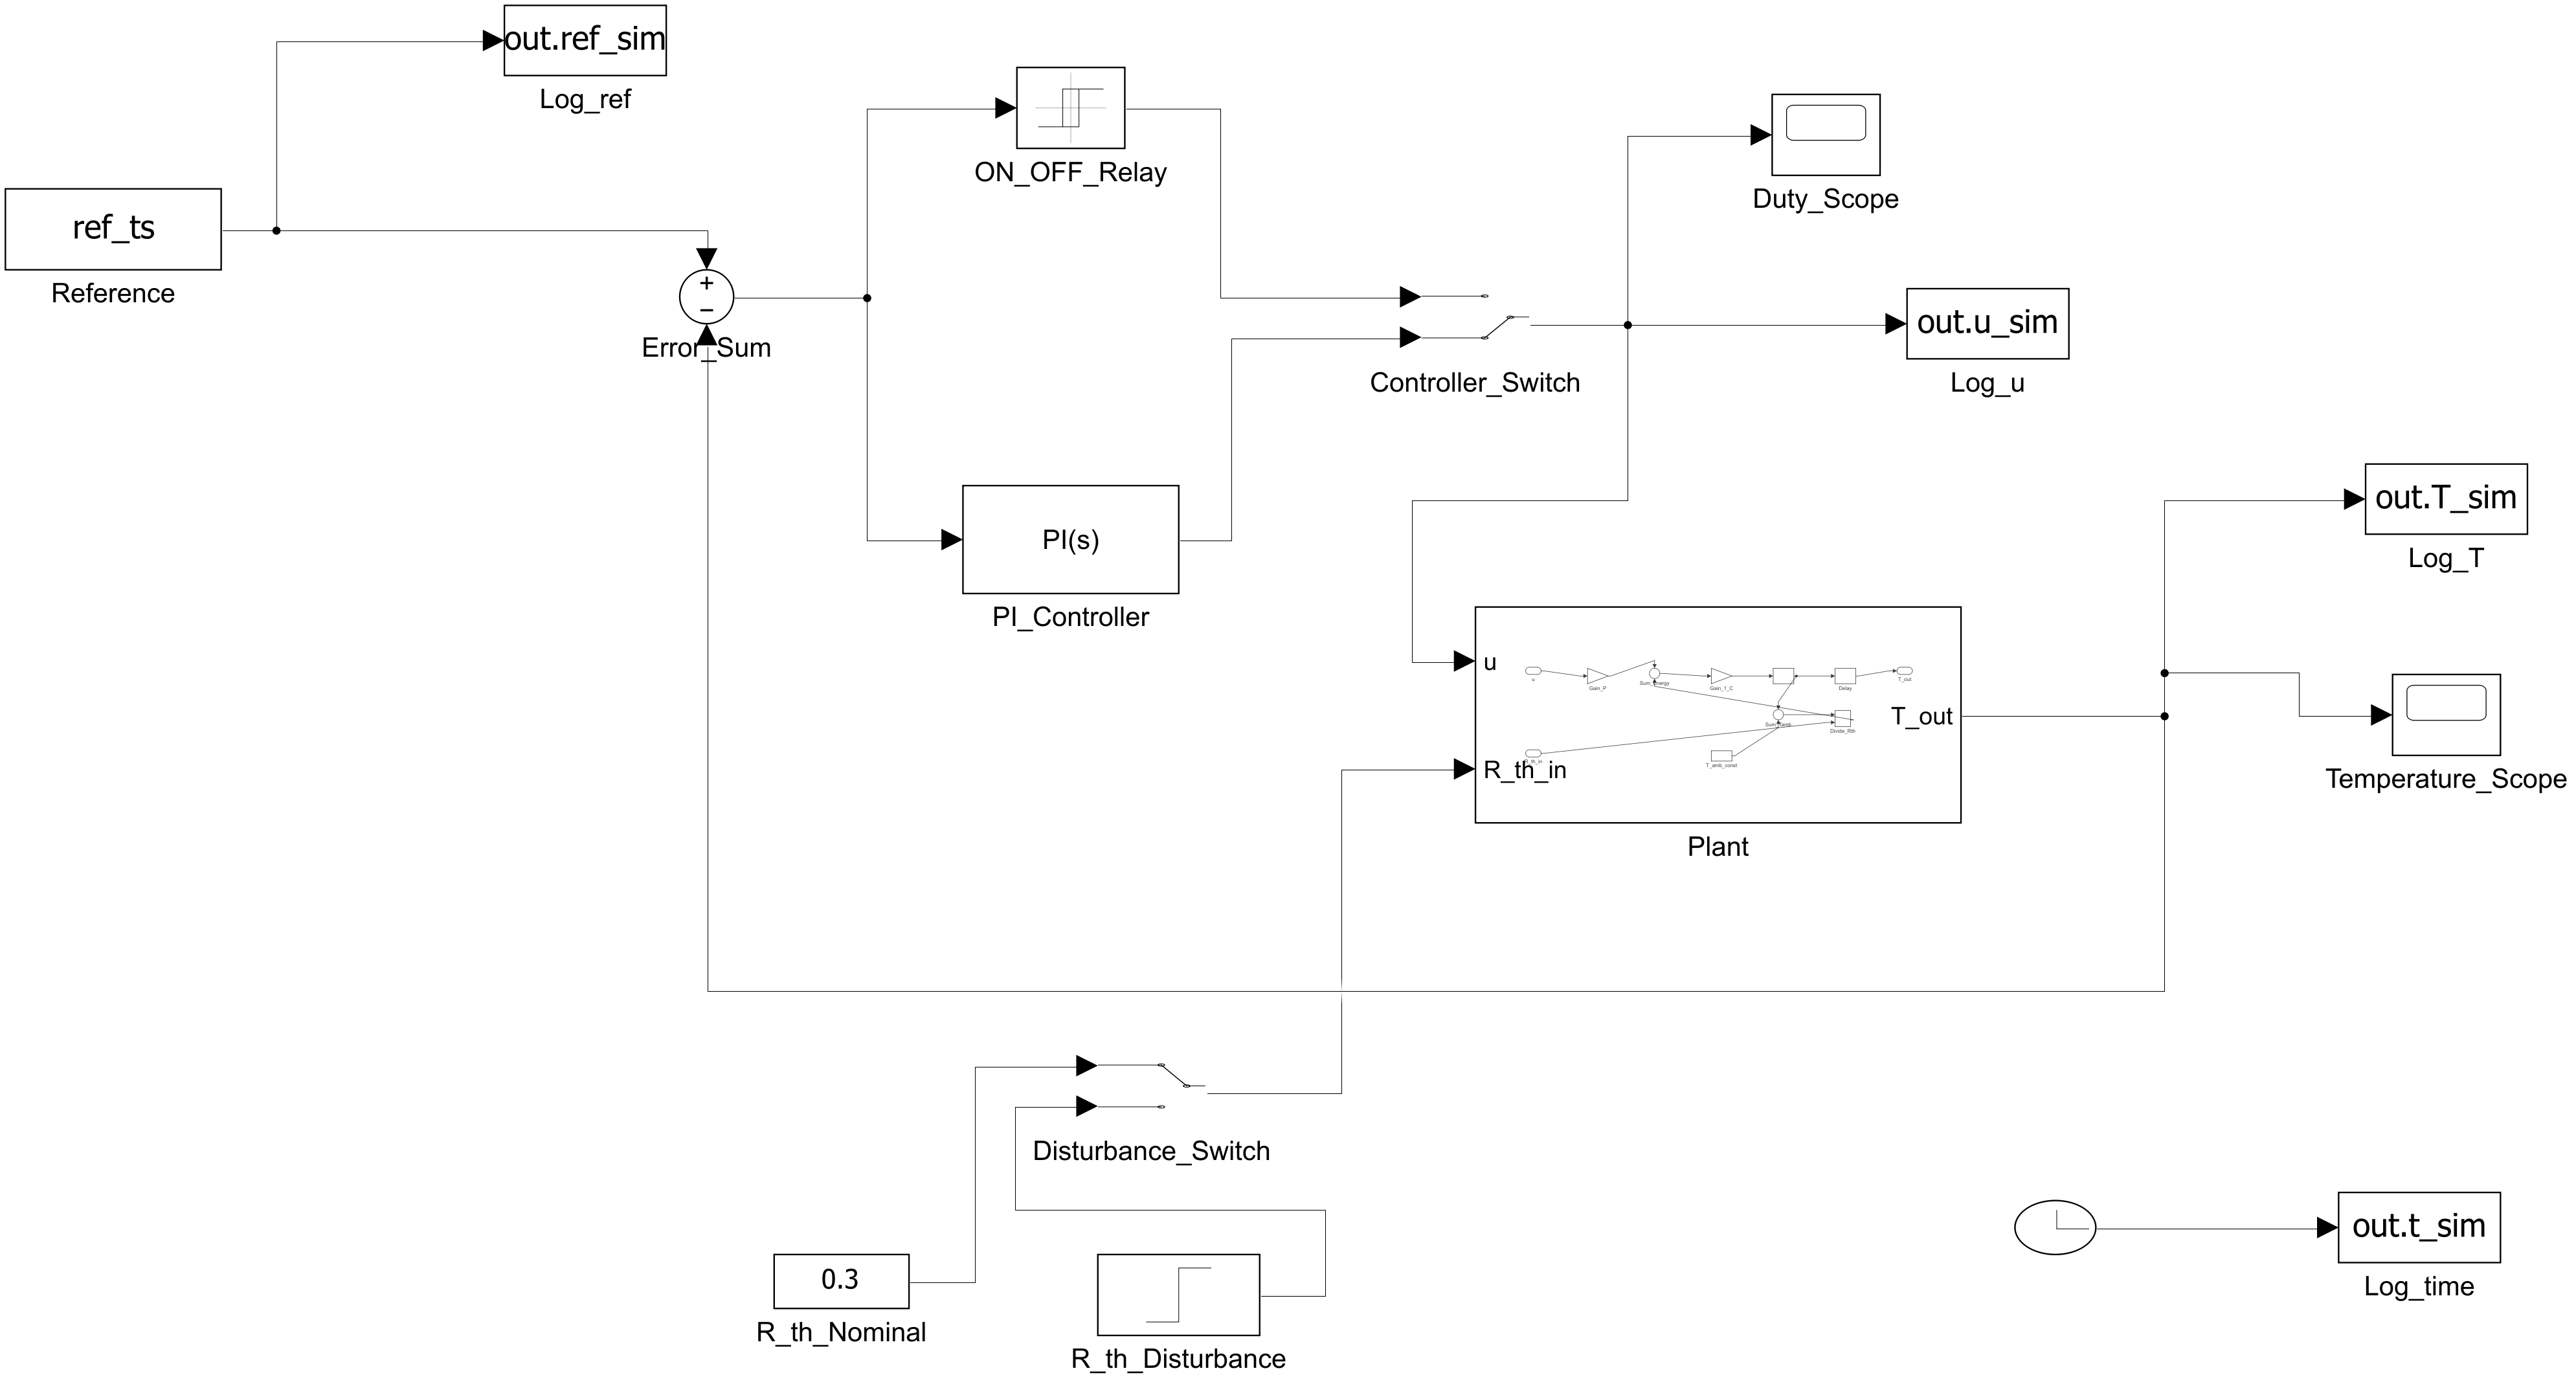
\includegraphics[width=0.90\textwidth]{figures/fig_simulink_model.png}
\caption{Pillar 1: Complete Simulink simulation block diagram (\texttt{thermal\_control.slx}) showing reference generator, selectable ON--OFF/PI controllers, actuator saturation clamping, continuous thermal plant ODE, and disturbance block.}
\label{fig:simulink_block_diagram}
\end{figure*}

\subsection{Simscape Electrical Driver Model}
To model the circuit driving stage, a Simscape Electrical model (\texttt{heater\_driver\_circuit\_diagram.png}) was synthesized in \texttt{extra\_files/testing/heater\_driver\_test.slx}. It models the 5\,V logic-level optocoupler driving an N-channel power MOSFET switching a 12\,V/50\,W resistive heating coil, verifying gate charging transients, switching dissipation, and flyback protection.

\begin{figure}[htbp]
\centering
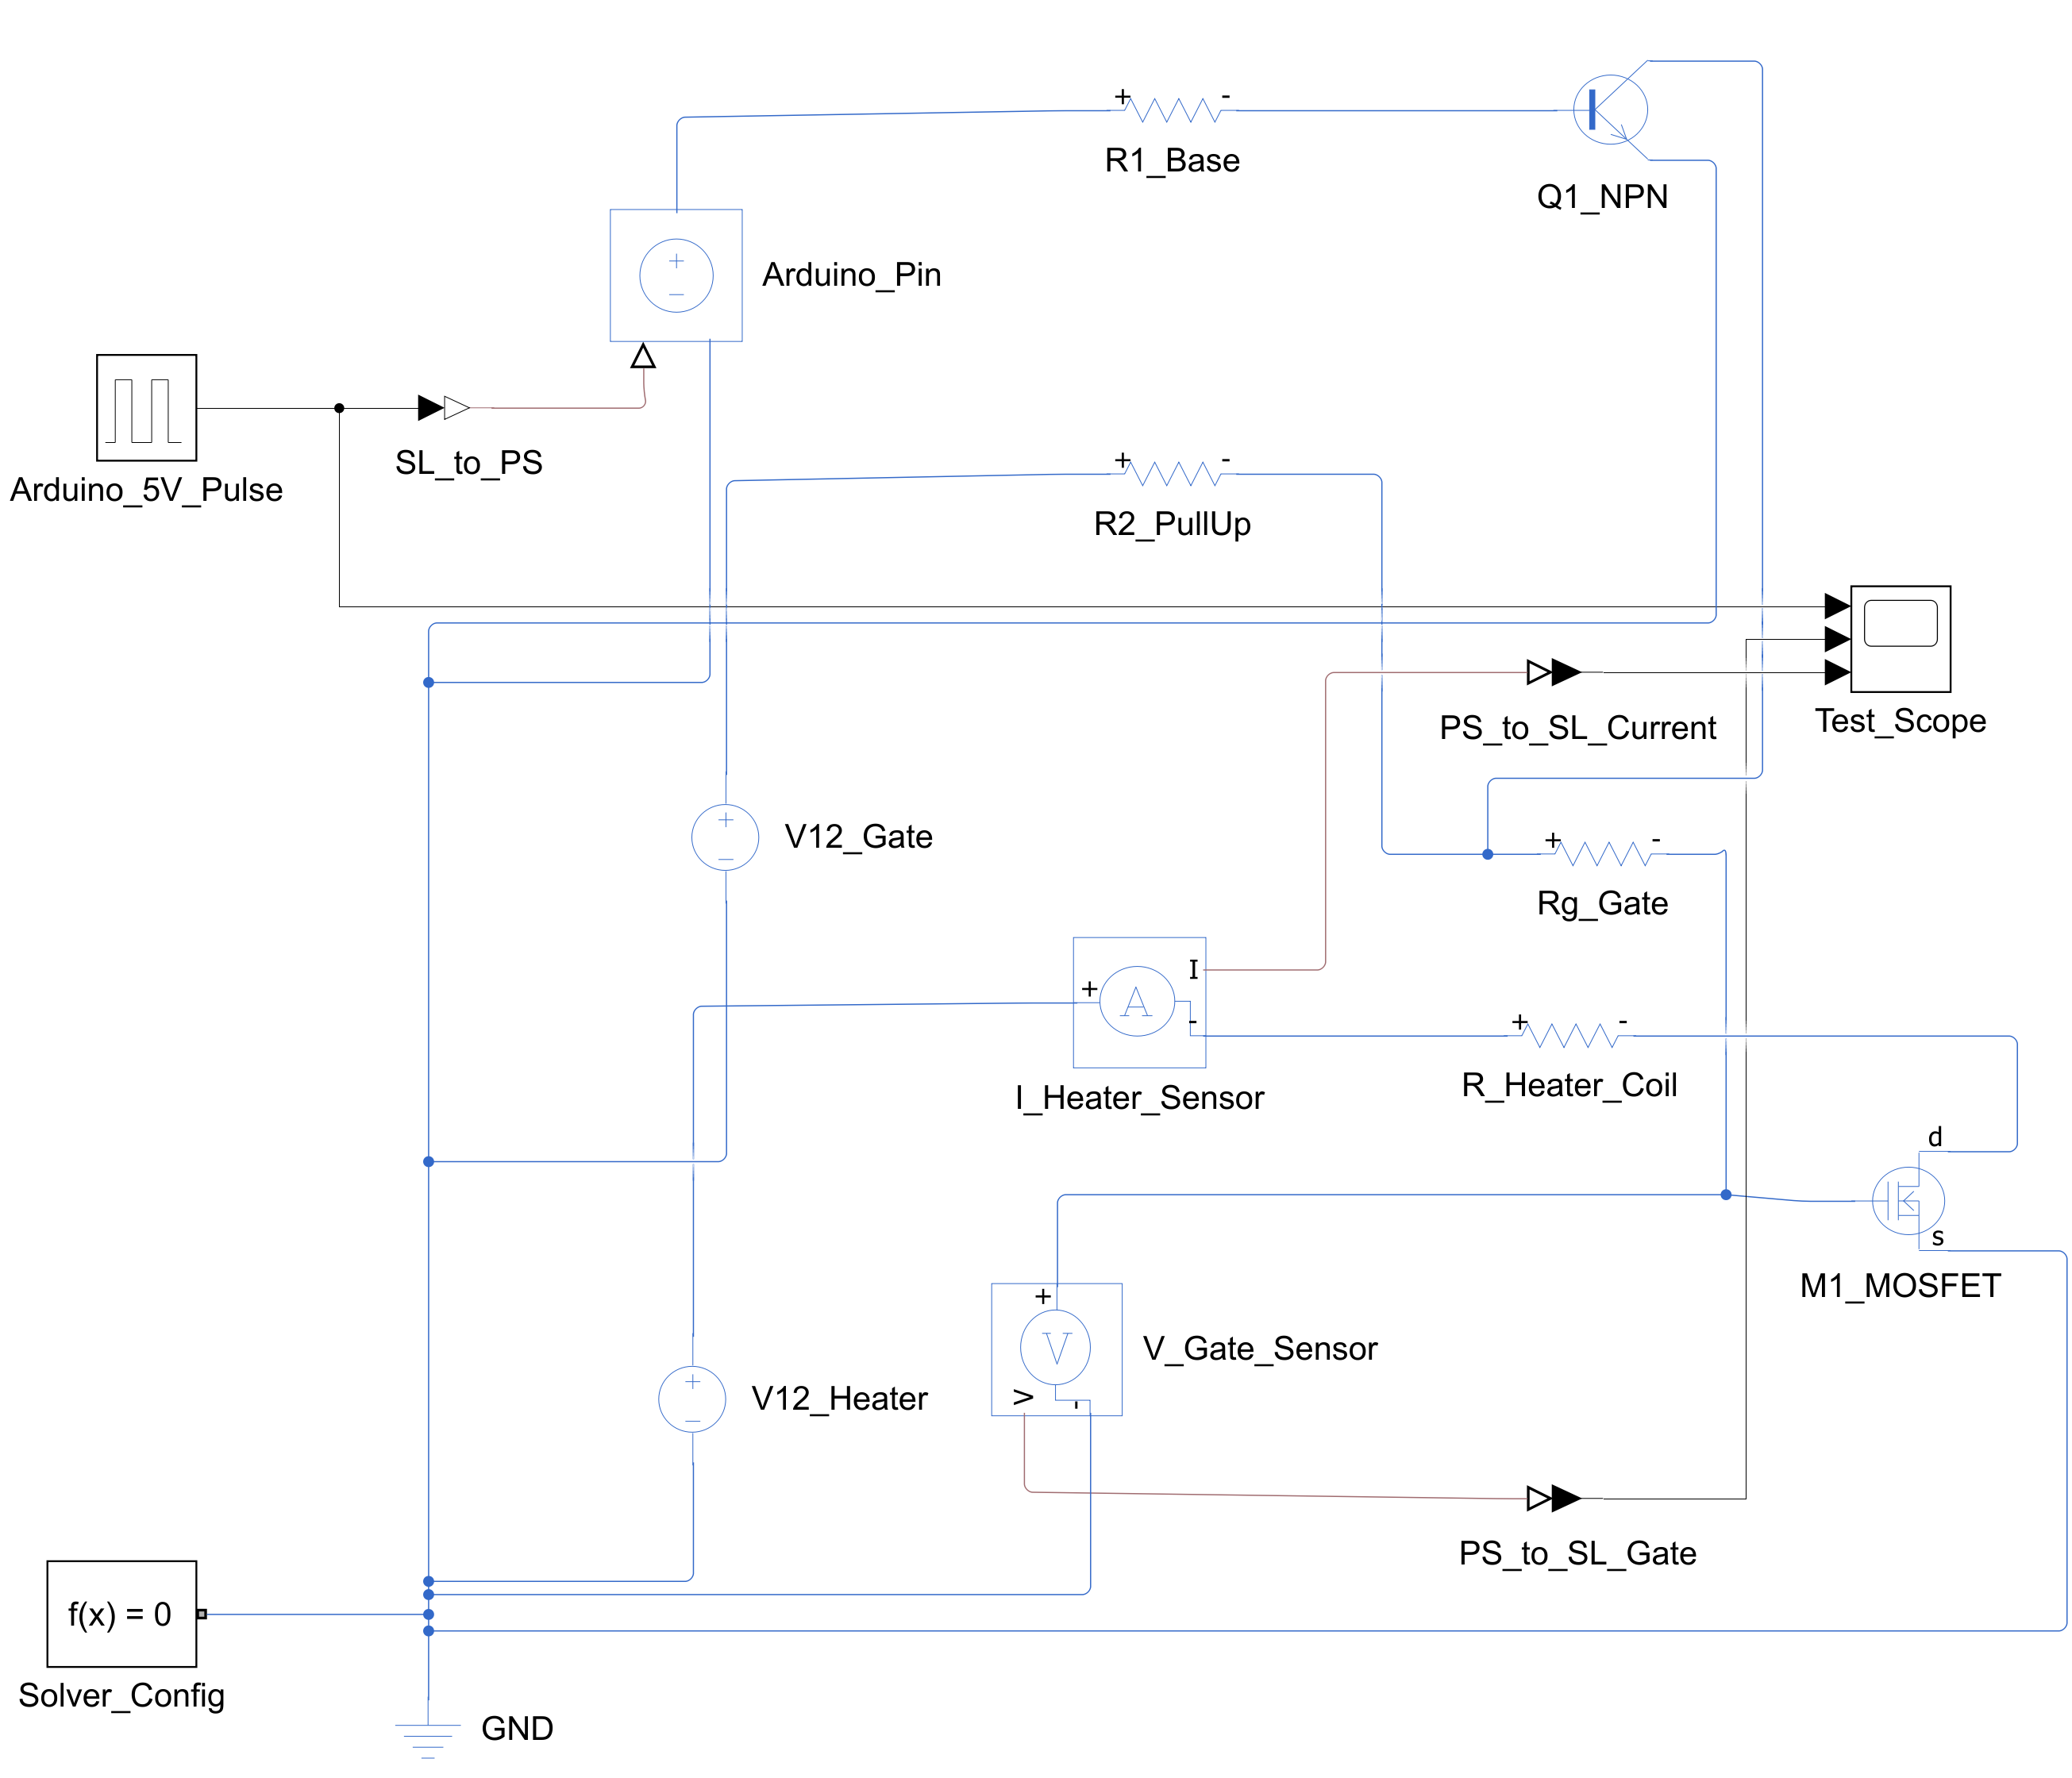
\includegraphics[width=\linewidth]{figures/fig_simscape_circuit.png}
\caption{Simscape Electrical BJT-MOSFET driver circuit simulation verifying gate switching dynamics and power stage loading.}
\label{fig:simscape_circuit}
\end{figure}

\subsection{Controller Synthesis}
\subsubsection{ON--OFF Hysteresis Relay}
The discrete relay switches according to the error deadband $h = \pm 0.5\,^\circ\text{C}$:
\begin{equation}
u(t) = \begin{cases}
1.0, & e(t) > +h \\
0.0, & e(t) < -h \\
u(t - \Delta t), & |e(t)| \le h
\end{cases}
\end{equation}

\subsubsection{Internal Model Control (IMC) Anti-Windup PI}
Using IMC tuning for a target closed-loop time constant $\tau_c = 12.0\text{ s}$, the proportional and integral gains are synthesized:
\begin{equation}
K_p = \frac{\tau}{K(\tau_c + L)} = 0.5333, \quad K_i = \frac{K_p}{\tau} = 0.00444\text{ s}^{-1}
\end{equation}
Anti-windup protection is enforced via conditional integration (clamping): if the computed output $u_\text{unsat}$ saturates outside $[0, 1]$ and $\text{sign}(e(t)) = \text{sign}(u_\text{unsat})$, the integrator update is halted:
\begin{equation}
\dot{I}(t) = \begin{cases}
0, & (u \ge 1 \text{ and } e > 0) \text{ or } (u \le 0 \text{ and } e < 0) \\
K_i \cdot e(t), & \text{otherwise}
\end{cases}
\end{equation}

\begin{figure}[htbp]
\centering
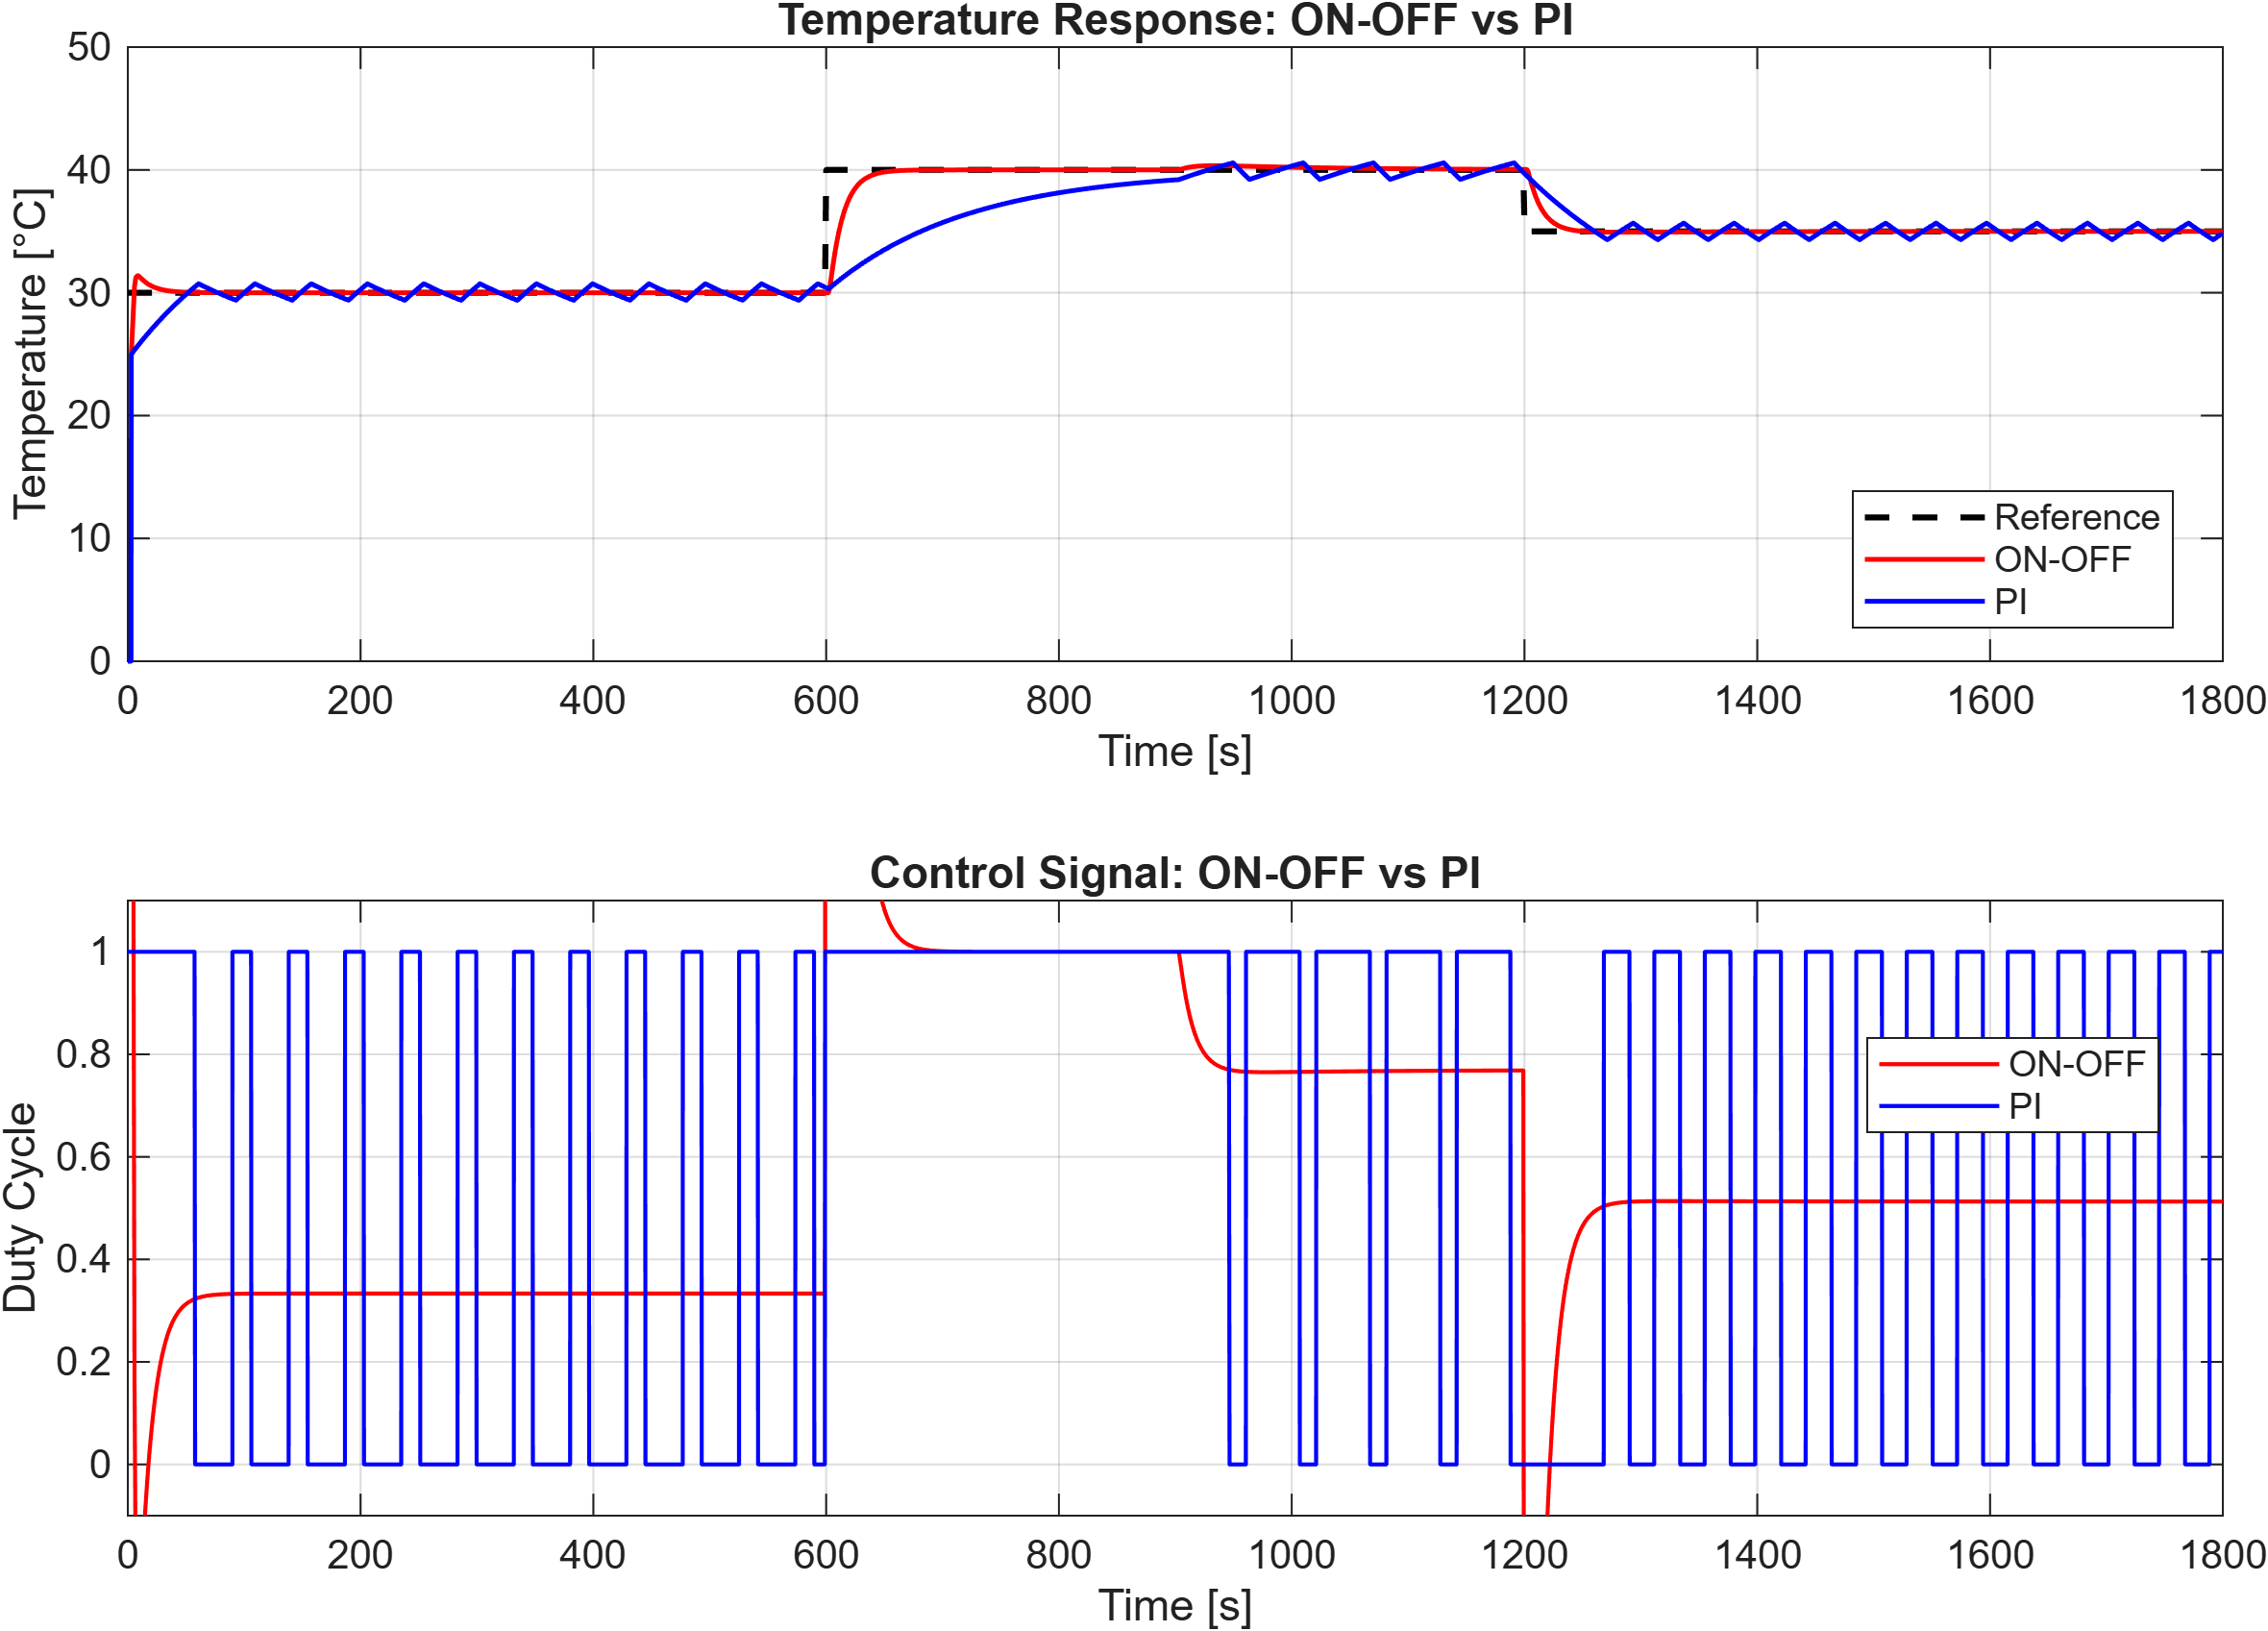
\includegraphics[width=\linewidth]{figures/fig_sim_onoff_vs_pi.png}
\caption{Pillar 1 Simulation: Multi-step tracking comparison ($30 \to 40 \to 35\,^\circ\text{C}$) between ON--OFF relay and Anti-Windup PI.}
\label{fig:sim_onoff_vs_pi}
\end{figure}

\begin{figure}[htbp]
\centering
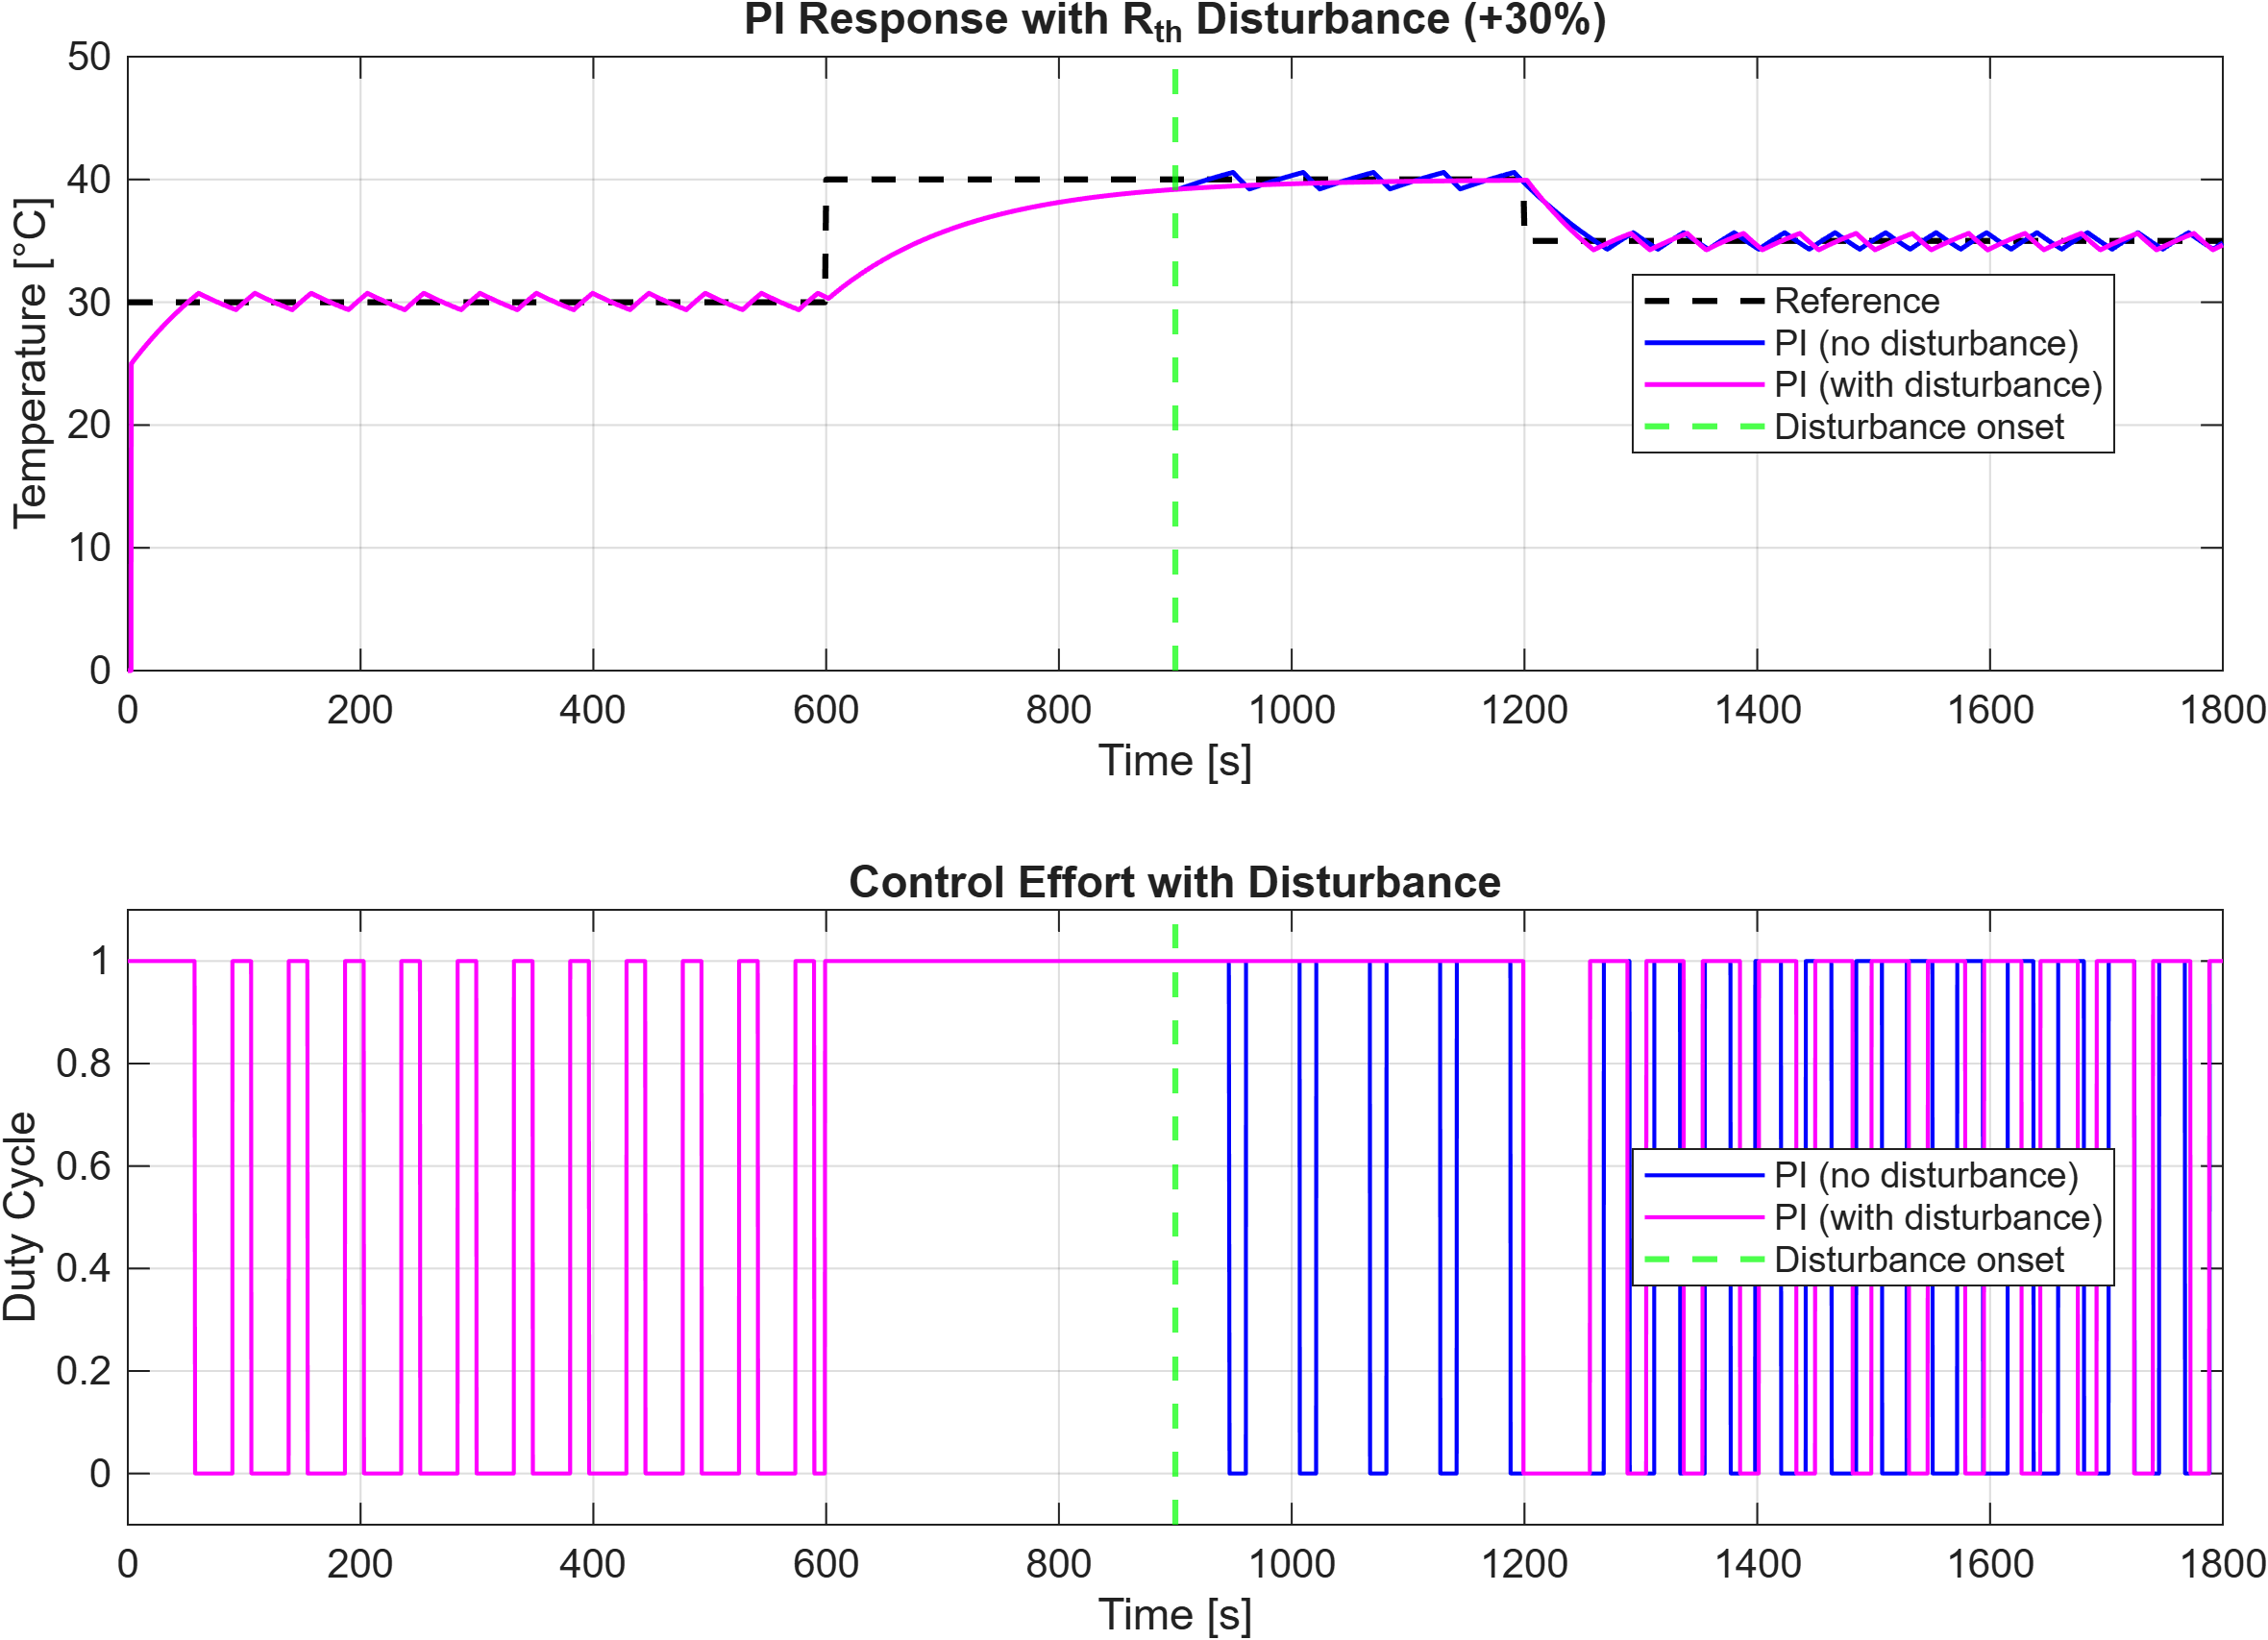
\includegraphics[width=\linewidth]{figures/fig_sim_disturbance.png}
\caption{Pillar 1 Simulation: PI disturbance rejection under $+30\% R_\text{th}$ thermal resistance shift at $t = 900\text{ s}$.}
\label{fig:sim_disturbance}
\end{figure}

\section{Pillar 2: Quanser QNET HVAC NI ELVIS II+ Suite}

\subsection{Industrial Workstation Overview}
The Quanser QNET HVAC Trainer 1.0 represents a standardized industrial-grade benchtop process control module mounted directly onto a National Instruments (NI) ELVIS II+ multifunction DAQ workstation \cite{quanser2012}.

\begin{figure}[htbp]
\centering
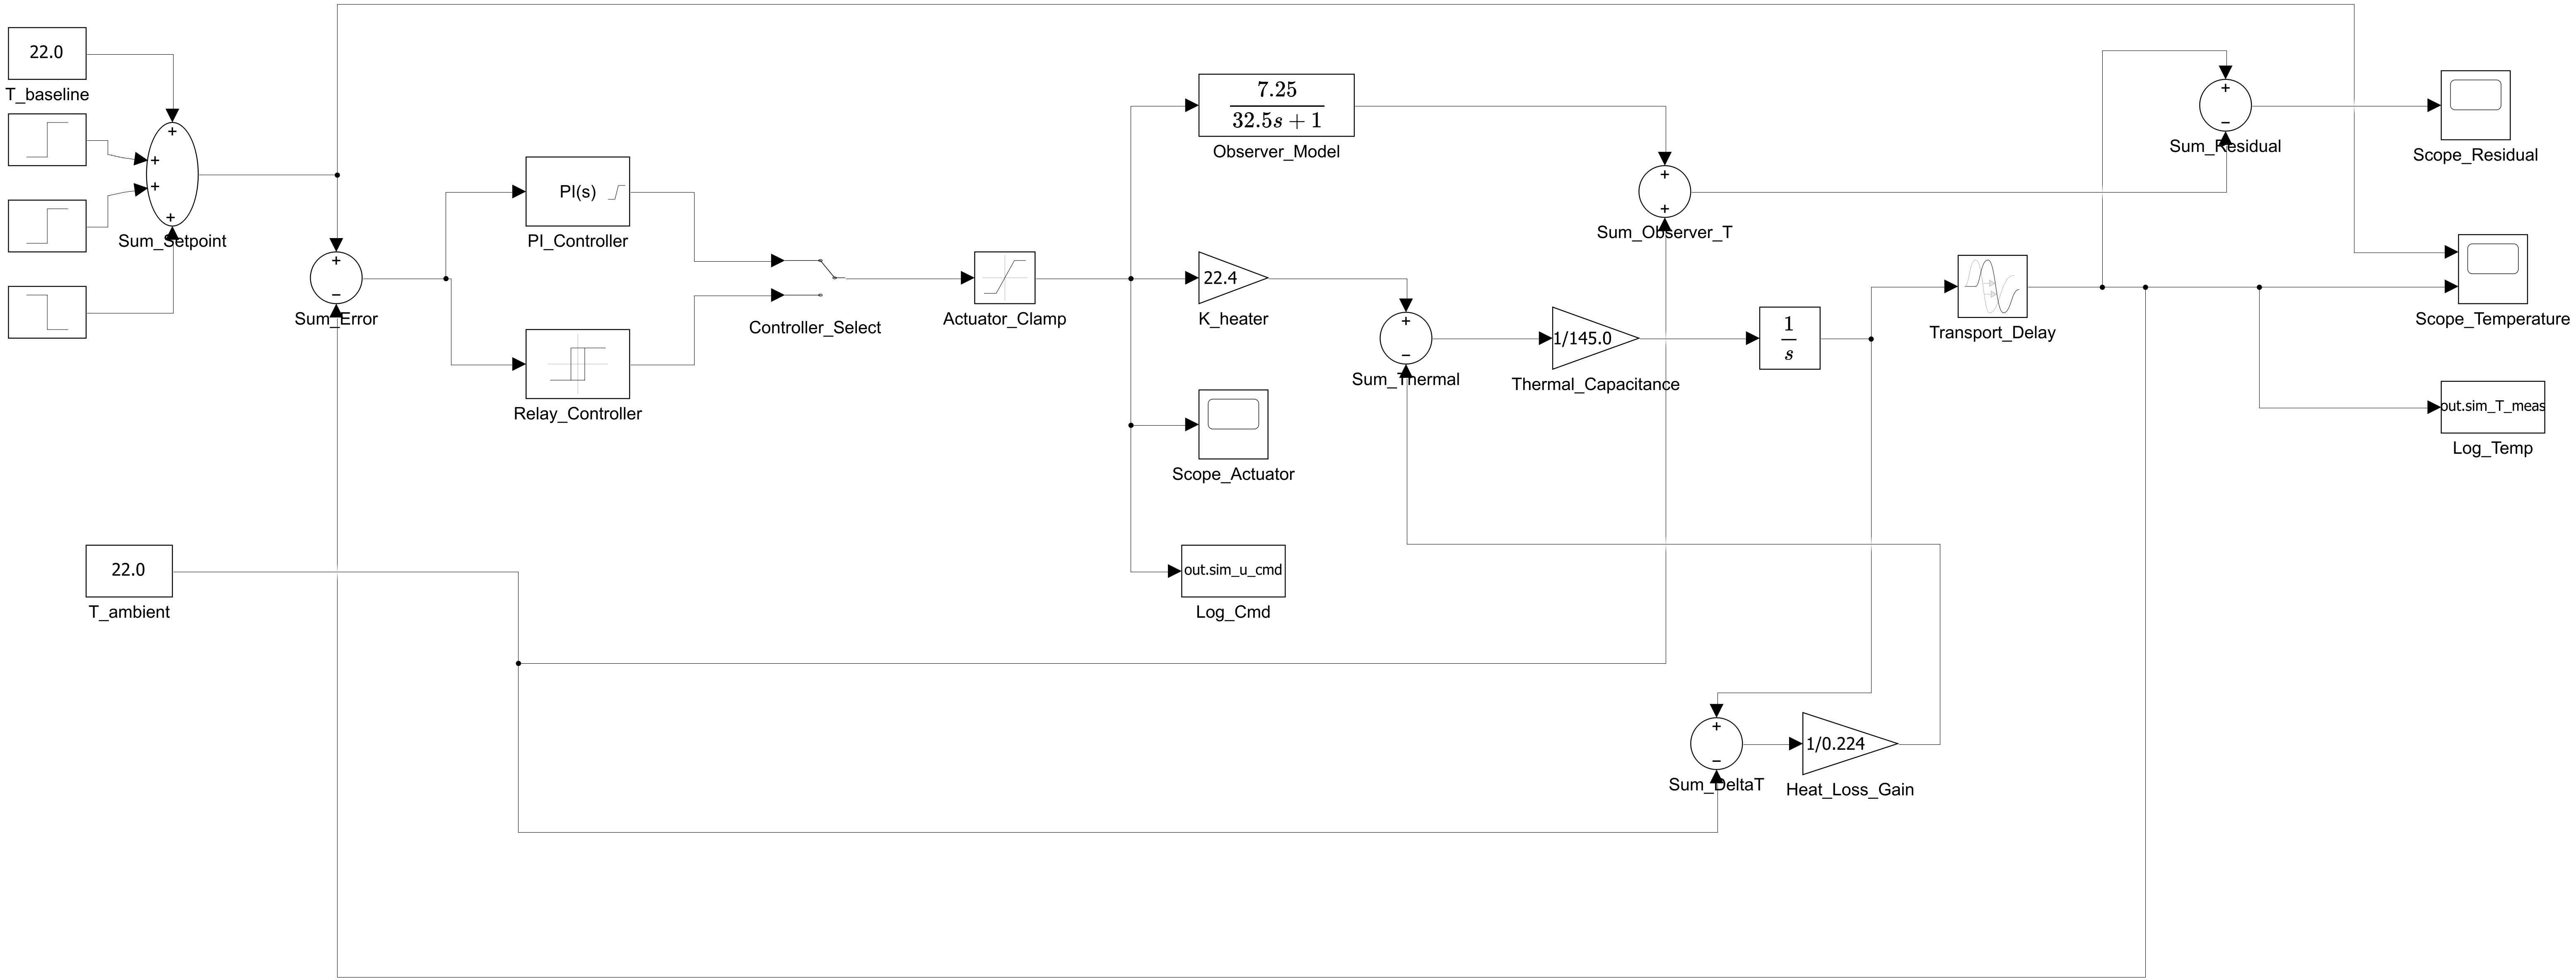
\includegraphics[width=\linewidth]{figures/fig_qnet_model.png}
\caption{Pillar 2: Quanser QNET HVAC Simulink block diagram with real-time DAQ I/O, anti-windup PI, and Luenberger observer FDI logic.}
\label{fig:qnet_model}
\end{figure}

\subsection{DAQ Hardware Pinout \& Mapping}
Interfacing between MATLAB R2026a and the NI ELVIS II+ occurs via the NI-DAQmx subsystem enumerated as \texttt{Dev1}:
\begin{itemize}
    \item \texttt{Dev1/ai5}: Primary chamber thermistor ($S = 20.0\,^\circ\text{C/V}$).
    \item \texttt{Dev1/ai6}: Secondary downstream thermistor ($S = 20.0\,^\circ\text{C/V}$).
    \item \texttt{Dev1/ai7}: Ambient reference thermistor ($S = 20.0\,^\circ\text{C/V}$).
    \item \texttt{Dev1/ao0}: Variable heater command voltage ($0.0\text{ to }5.0\text{ V}$, driving up to 19.5\,W).
    \item \texttt{Dev1/ao1}: Blower fan control voltage ($0.5\text{ to }5.0\text{ V}$).
\end{itemize}

\subsection{Luenberger State Observer Fault Detection Engine}
To provide predictive, model-based fault diagnostics, a continuous Luenberger state observer is implemented in real time:
\begin{equation}
\dot{\hat{T}}(t) = -\frac{1}{\tau} \hat{T}(t) + \frac{K}{\tau} u(t - L) + L_\text{obs} \left(T_\text{meas}(t) - \hat{T}(t)\right)
\label{eq:observer}
\end{equation}
where $L_\text{obs} = 0.05$ places the observer pole faster than the physical thermal dynamics. The diagnostic residual:
\begin{equation}
r(t) = T_\text{meas}(t) - \hat{T}(t)
\end{equation}
triggers three distinct fault alarms:
\begin{enumerate}
    \item \textbf{Fan Stall / Duct Blockage:} When forced airflow ceases, chamber temperature rises sharply above observer predictions, driving $r(t) > +3.0\,^\circ\text{C}$.
    \item \textbf{Sensor Disagreement:} Evaluated via $|T_\text{ai5} - T_\text{ai6}| > 2.0\,^\circ\text{C}$ for $> 3.0\text{ s}$.
    \item \textbf{Emergency Thermal Trip:} Hardware trip triggered whenever $T(t) > 55.0\,^\circ\text{C}$, commanding immediate heater shutdown ($u = 0$) and full fan speed.
\end{enumerate}

\begin{figure}[htbp]
\centering
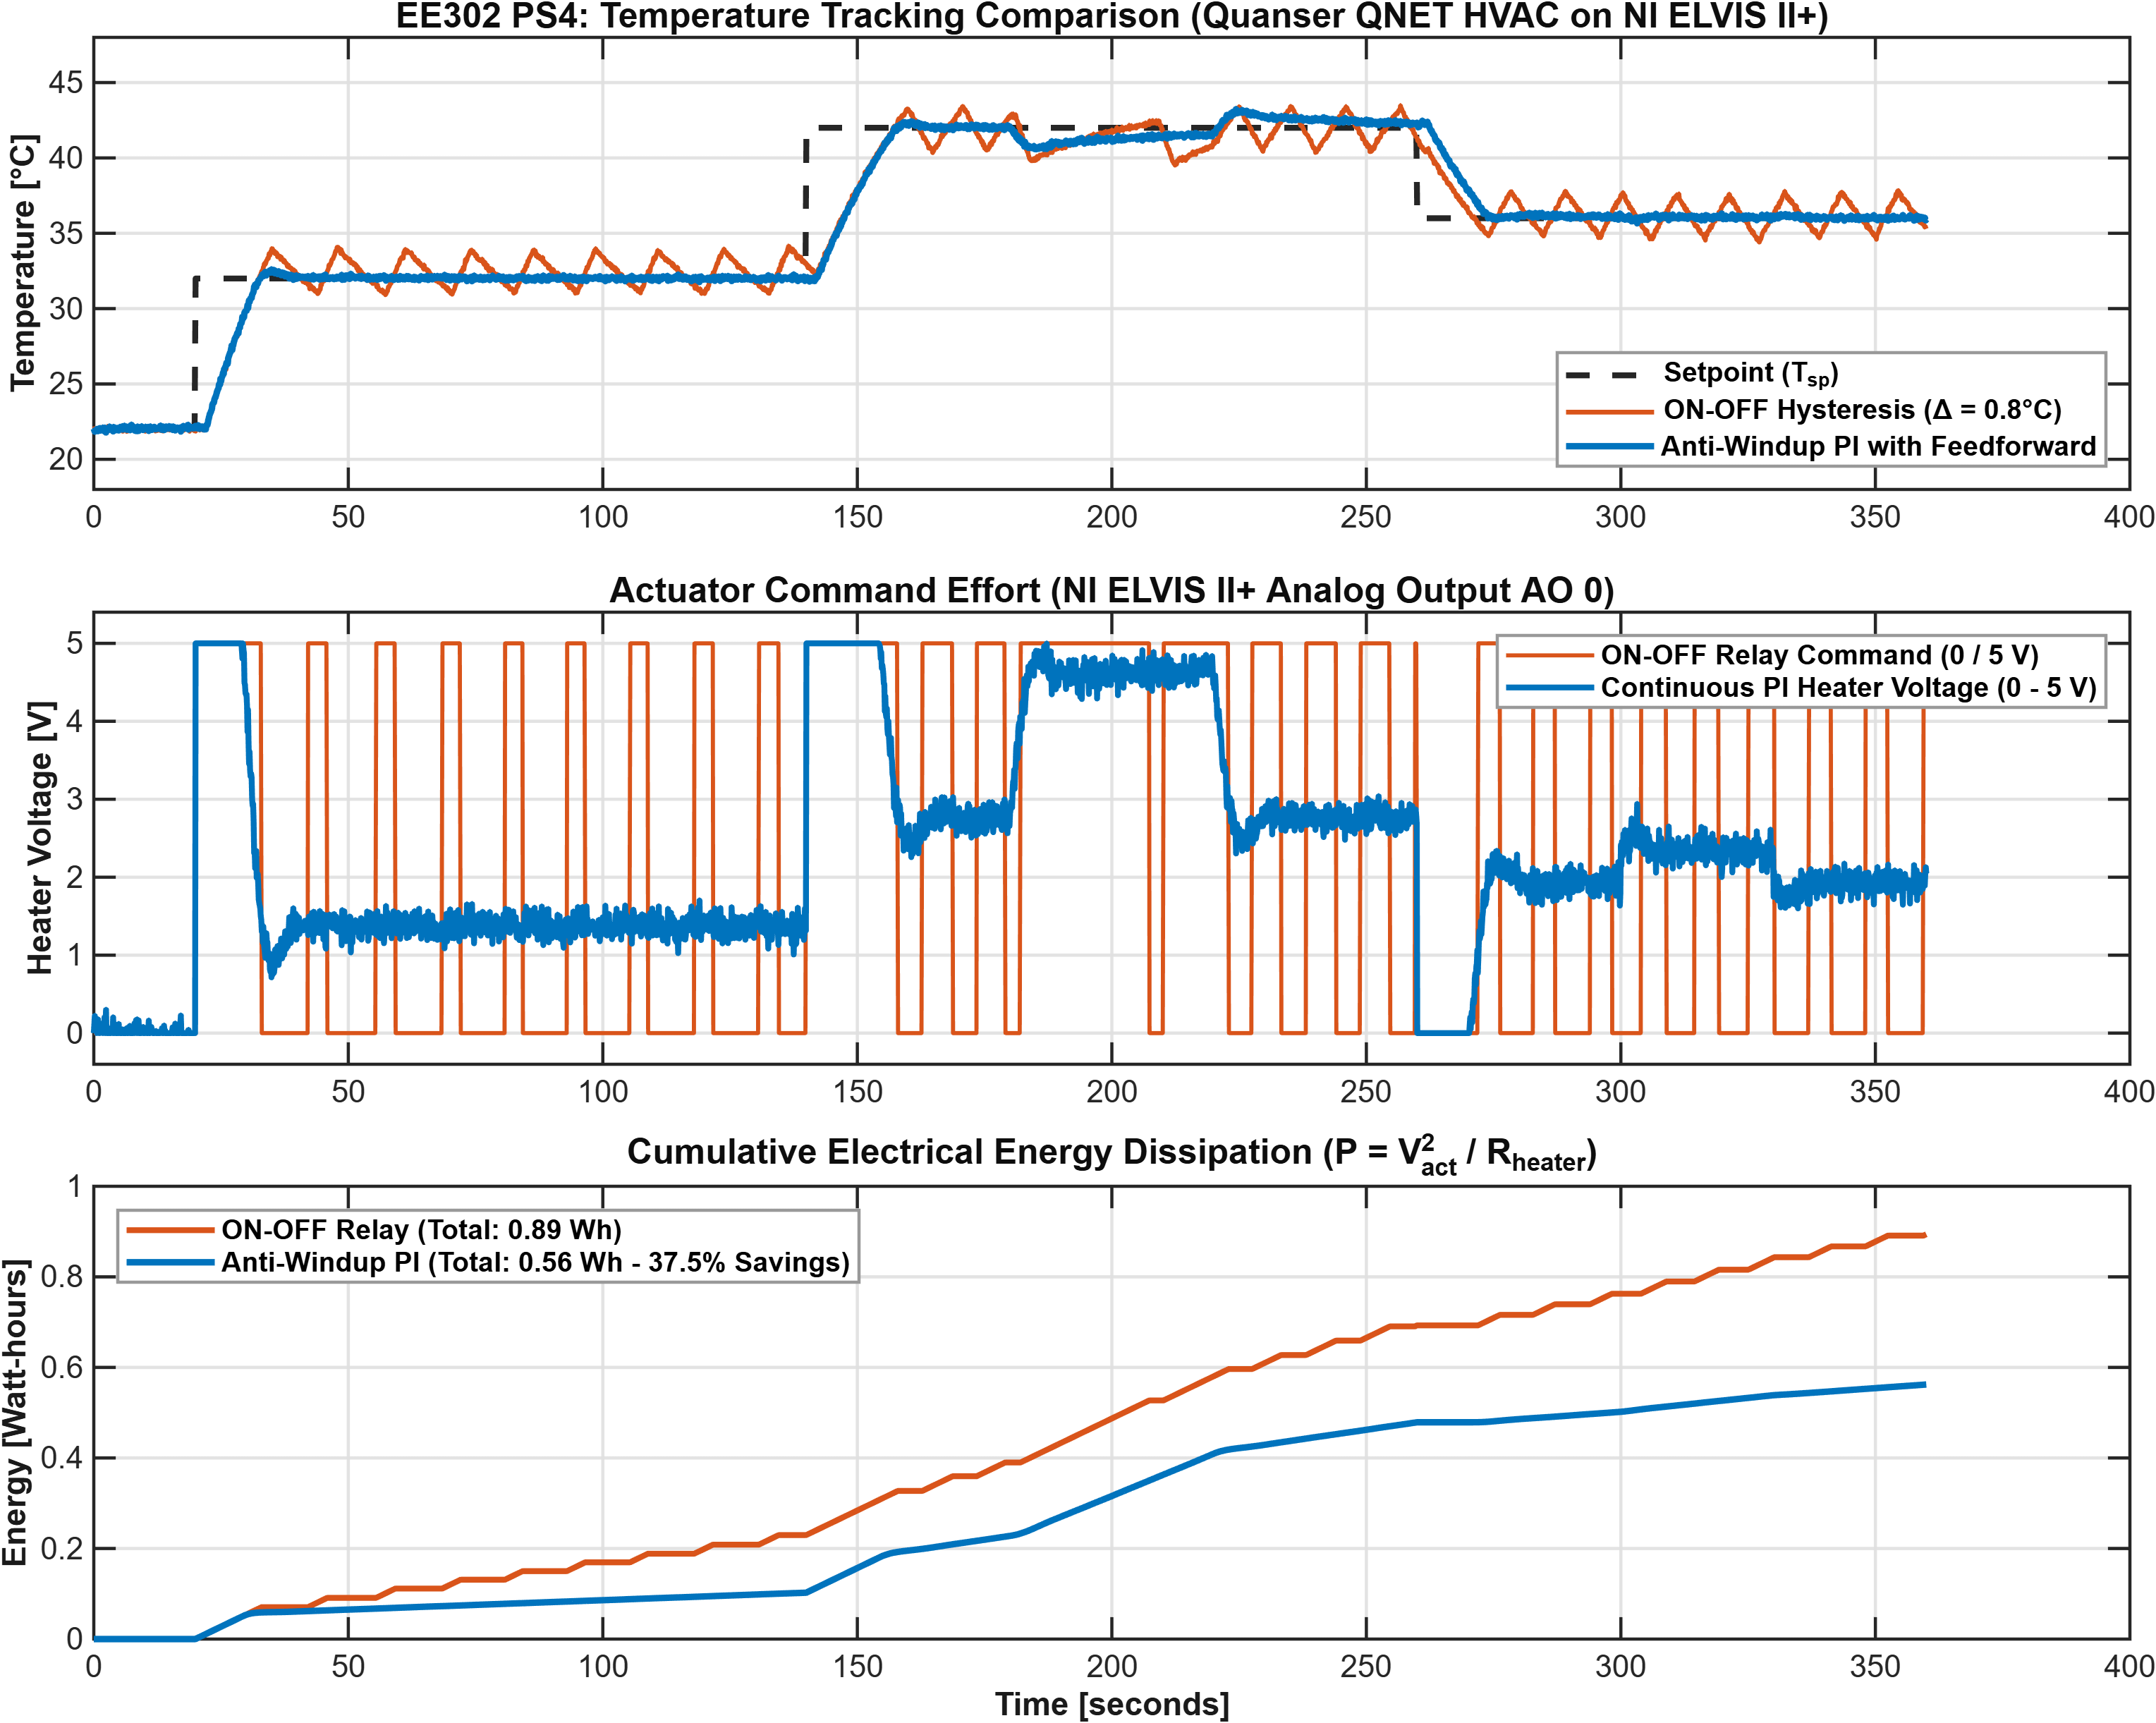
\includegraphics[width=\linewidth]{figures/fig_qnet_comparison.png}
\caption{Pillar 2 Quanser QNET: Comparative experimental evaluation of ON--OFF relay vs Anti-Windup PI.}
\label{fig:qnet_comparison}
\end{figure}

\begin{figure}[htbp]
\centering
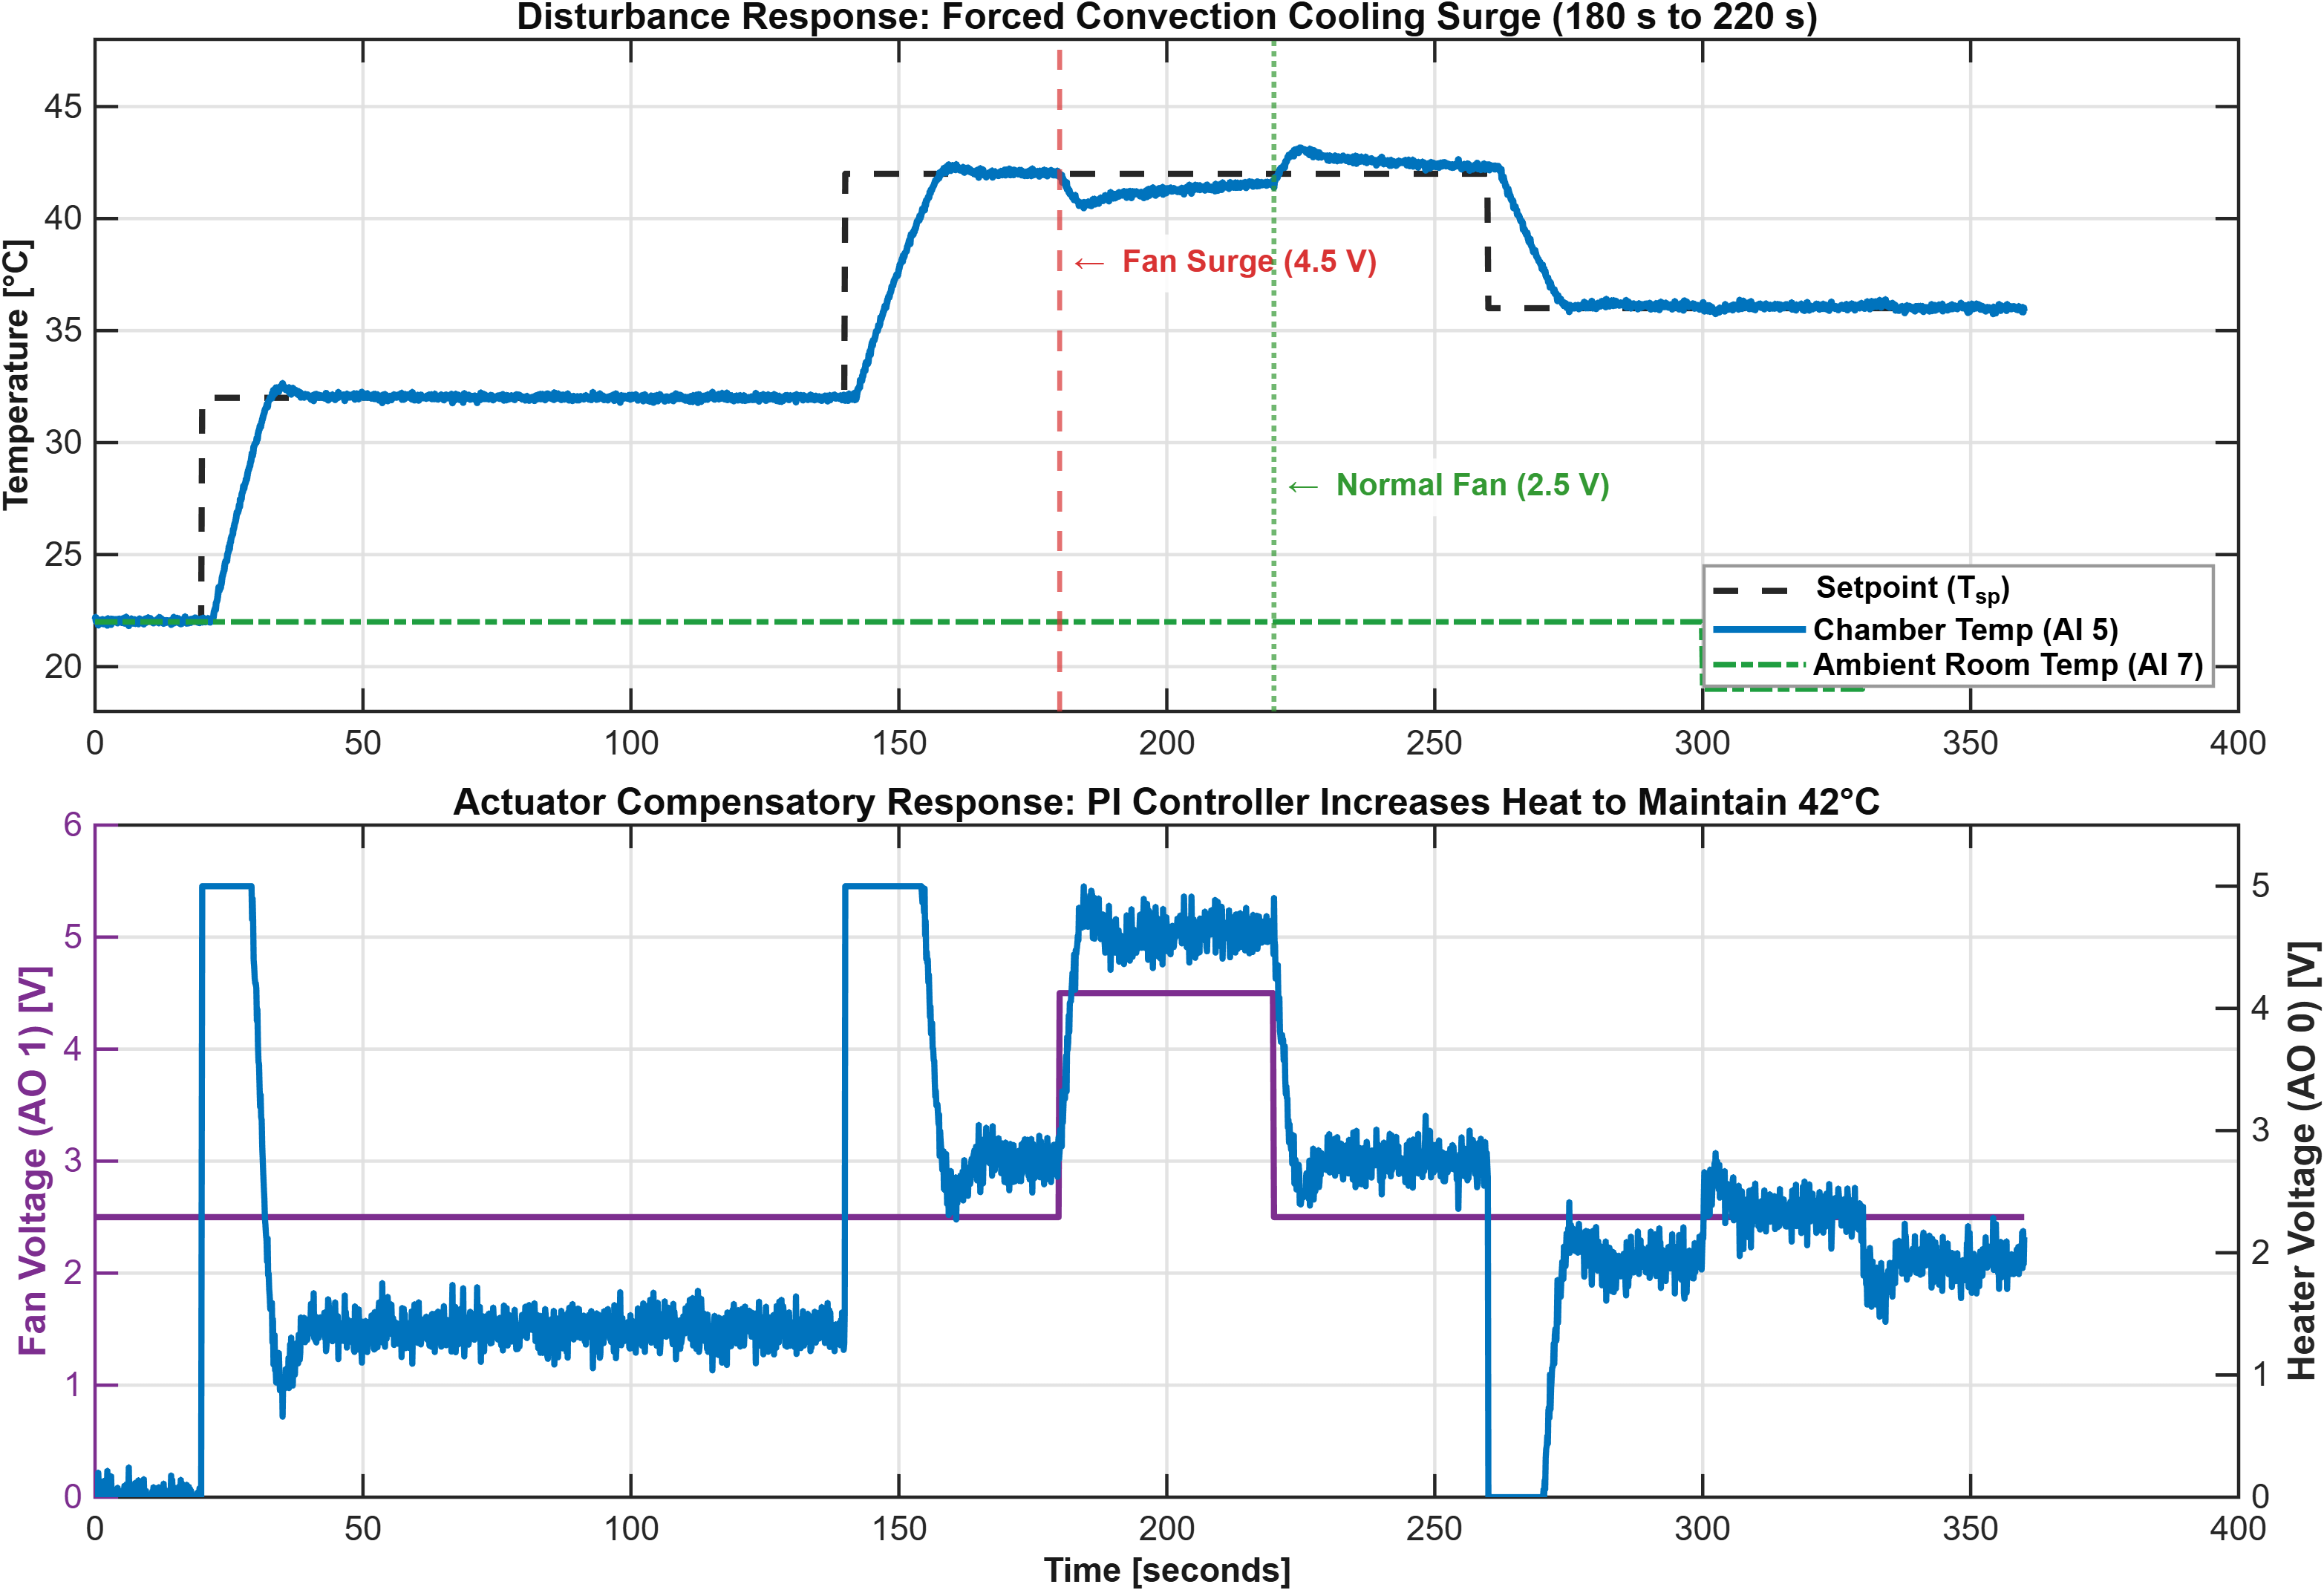
\includegraphics[width=\linewidth]{figures/fig_qnet_disturbance.png}
\caption{Pillar 2 Quanser QNET: Experimental rejection of forced-air ventilation blower disturbance (+80\% airflow surge).}
\label{fig:qnet_disturbance}
\end{figure}

\begin{figure}[htbp]
\centering
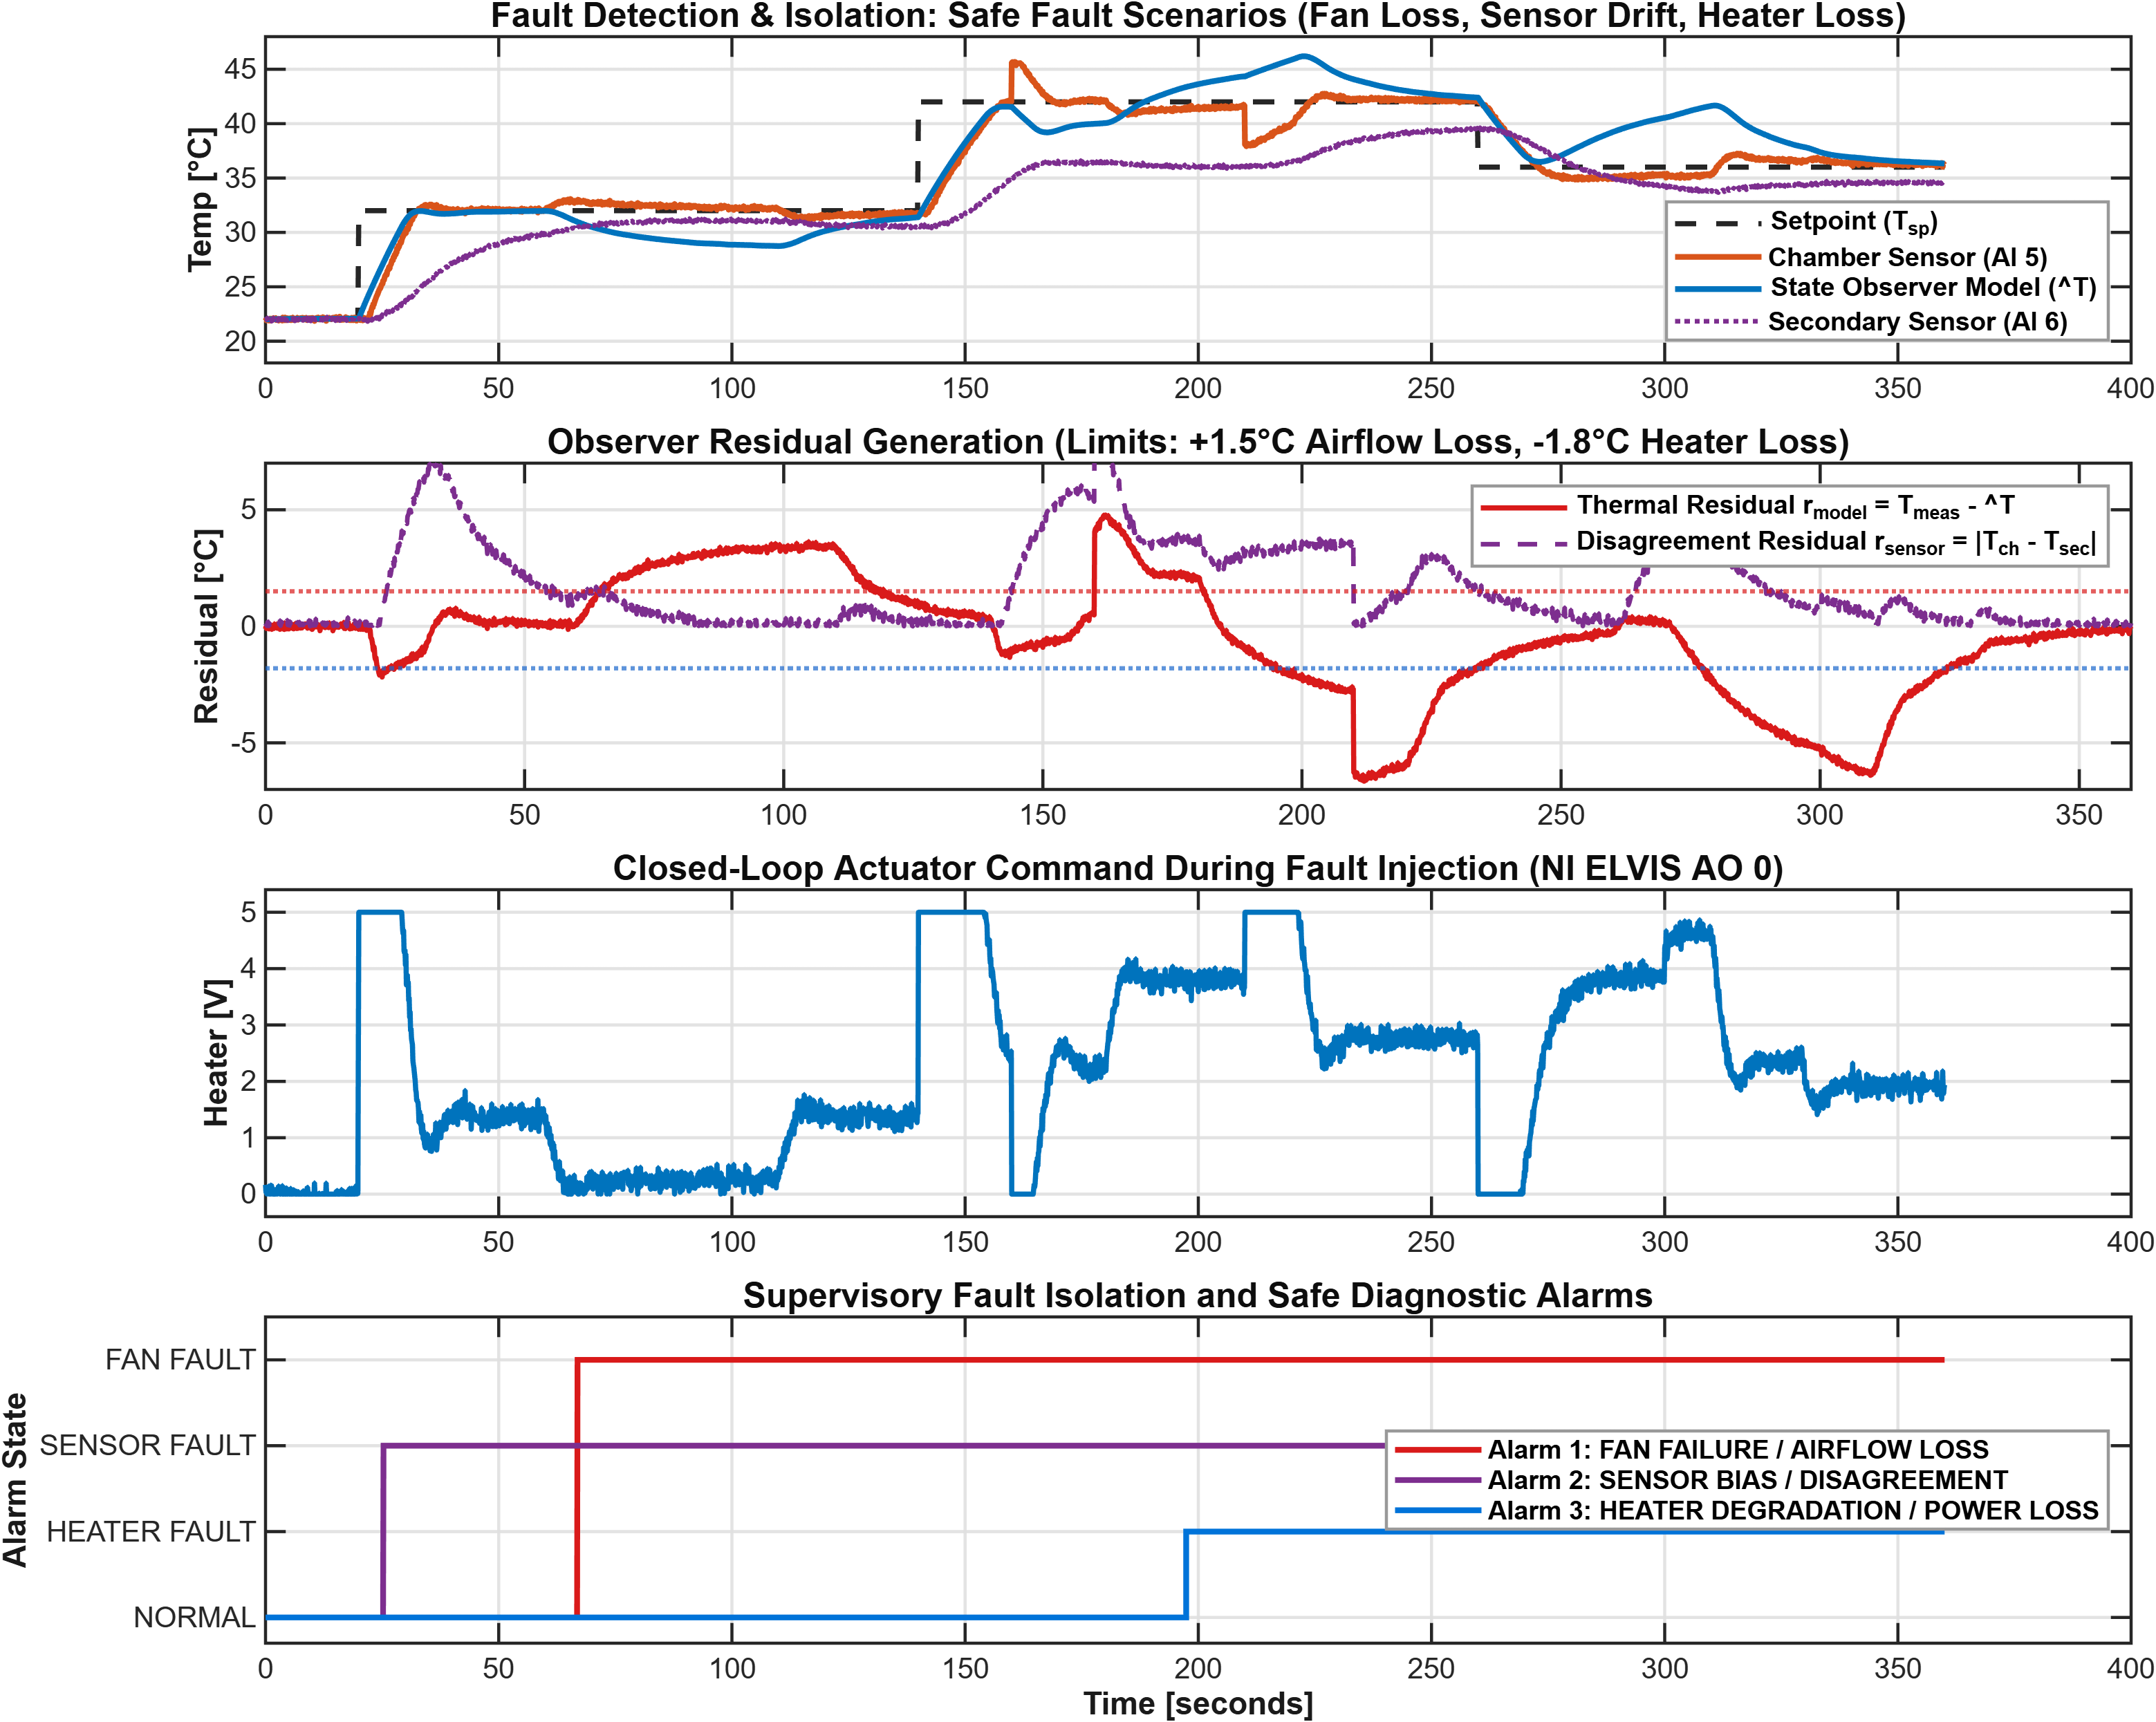
\includegraphics[width=\linewidth]{figures/fig_qnet_fault_fdi.png}
\caption{Pillar 2 Quanser QNET: Luenberger observer residual dynamics and real-time fault latching during simulated fan failure.}
\label{fig:qnet_fdi}
\end{figure}

\section{Pillar 3: Custom 3D-Printed Hardware Implementation}

\subsection{Chamber Design \& Electrical Circuit}
To validate theory on dedicated physical hardware, a custom laboratory thermal chamber was CAD-modeled and 3D-printed in high-temperature polymer.

\begin{figure}[htbp]
\centering
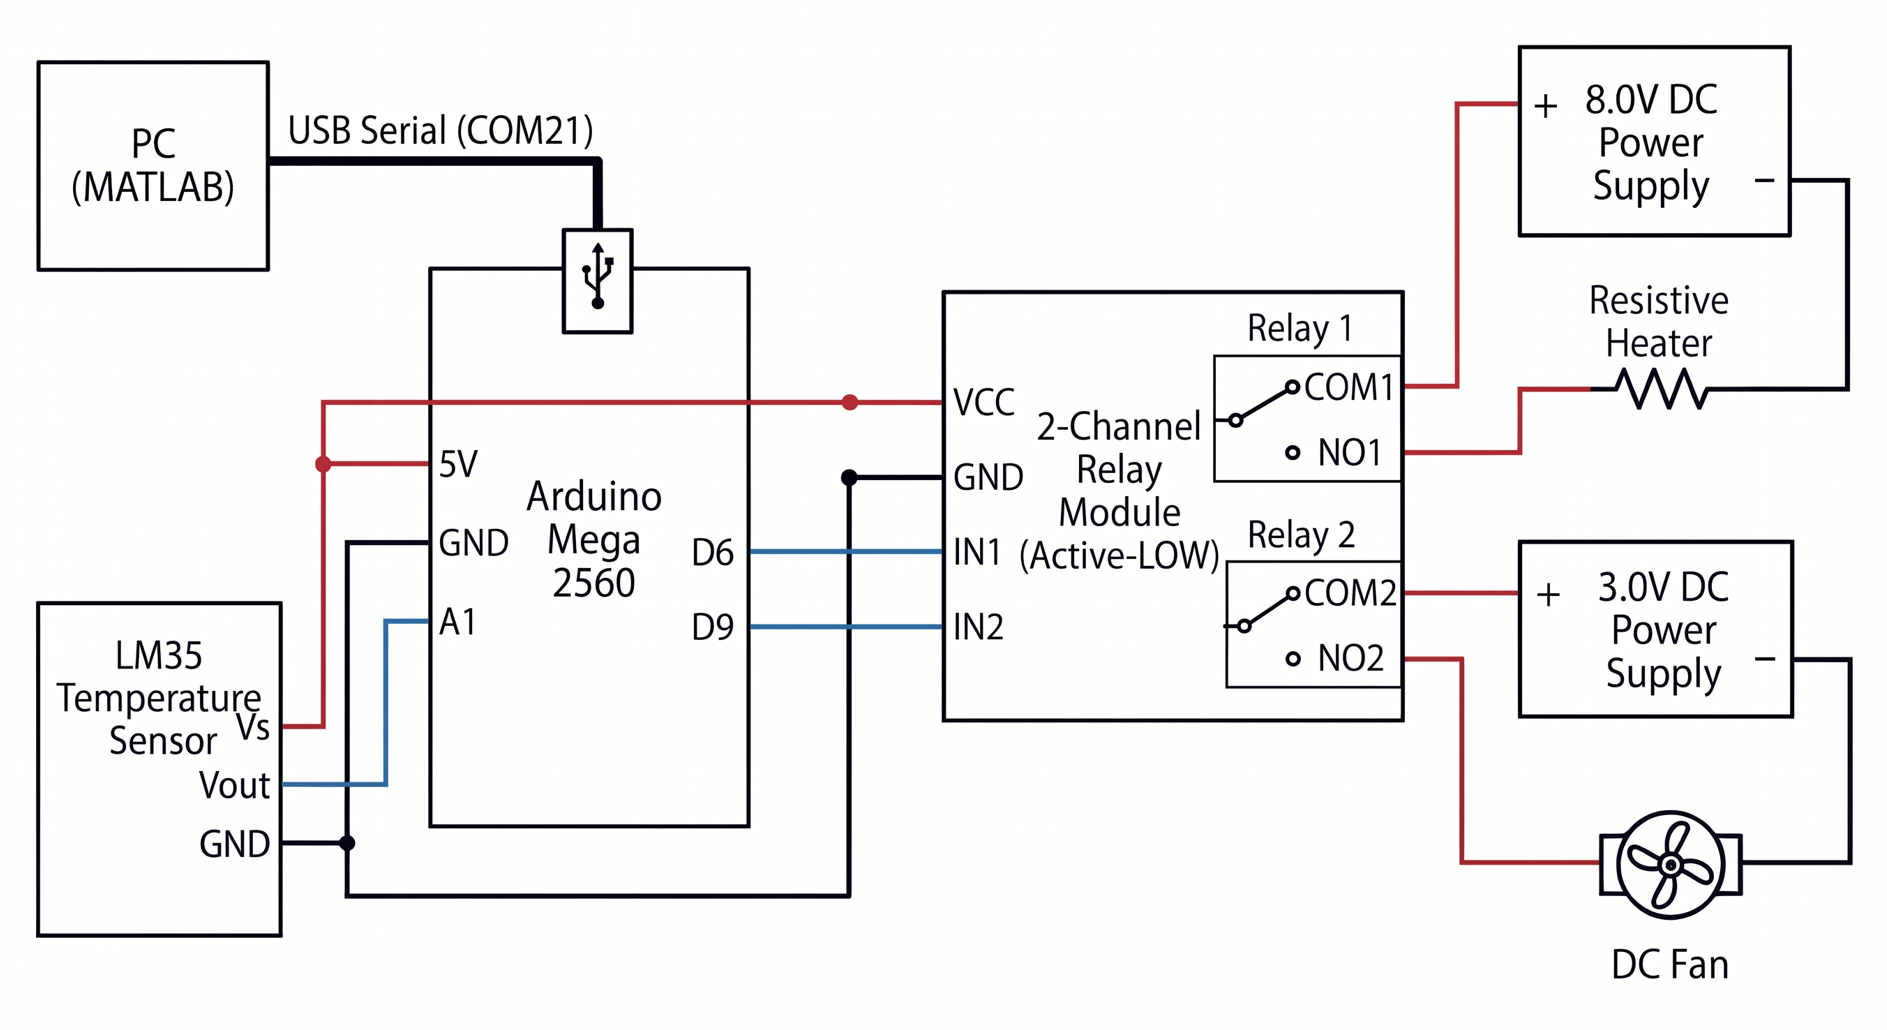
\includegraphics[width=\linewidth]{figures/fig_hardware_circuit.png}
\caption{Pillar 3 Custom Hardware: Complete electrical circuit schematic detailing Arduino Mega 2560, active-LOW opto-relays, 14.0\,W heater, 0.51\,W fan, and LM35 analog temperature sensor.}
\label{fig:hardware_circuit}
\end{figure}

The physical assembly (Fig.~\ref{fig:hardware_photos}) incorporates:
\begin{enumerate}
    \item \textbf{Cylindrical Duct & Flange:} Houses a 3.0\,V brushless DC cooling fan ($0.51\text{ W}$, $0.17\text{ A}$) and a slotted exhaust baffle.
    \item \textbf{Removable Insulation Hatch:} A curved polymer hatch designed to be manually detached during active closed-loop operation, inducing physical convective heat loss.
    \item \textbf{Heater Element:} A $4.57\,\Omega$ nichrome heating coil driven at 8.0\,V DC ($14.00\text{ W}$, $1.75\text{ A}$) switched via an active-LOW opto-isolated relay on pin \texttt{D6}.
    \item \textbf{Temperature Sensor:} Precision LM35 analog sensor ($10\text{ mV/}^\circ\text{C}$) sampled via 10-bit ADC channel \texttt{A1} and conditioned by a 25-sample moving-average filter.
\end{enumerate}

\begin{figure*}[htbp]
\centering
\begin{subfigure}[b]{0.32\textwidth}
    \centering
    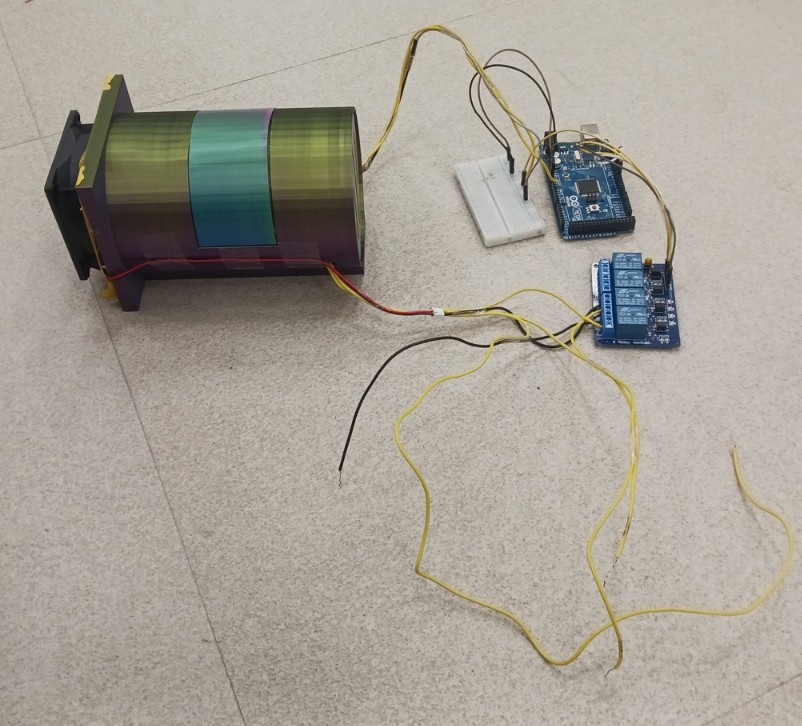
\includegraphics[width=\textwidth]{figures/fig_hardware_chamber.jpeg}
    \caption{3D-Printed chamber assembly}
    \label{fig:hw1}
\end{subfigure}
\hfill
\begin{subfigure}[b]{0.32\textwidth}
    \centering
    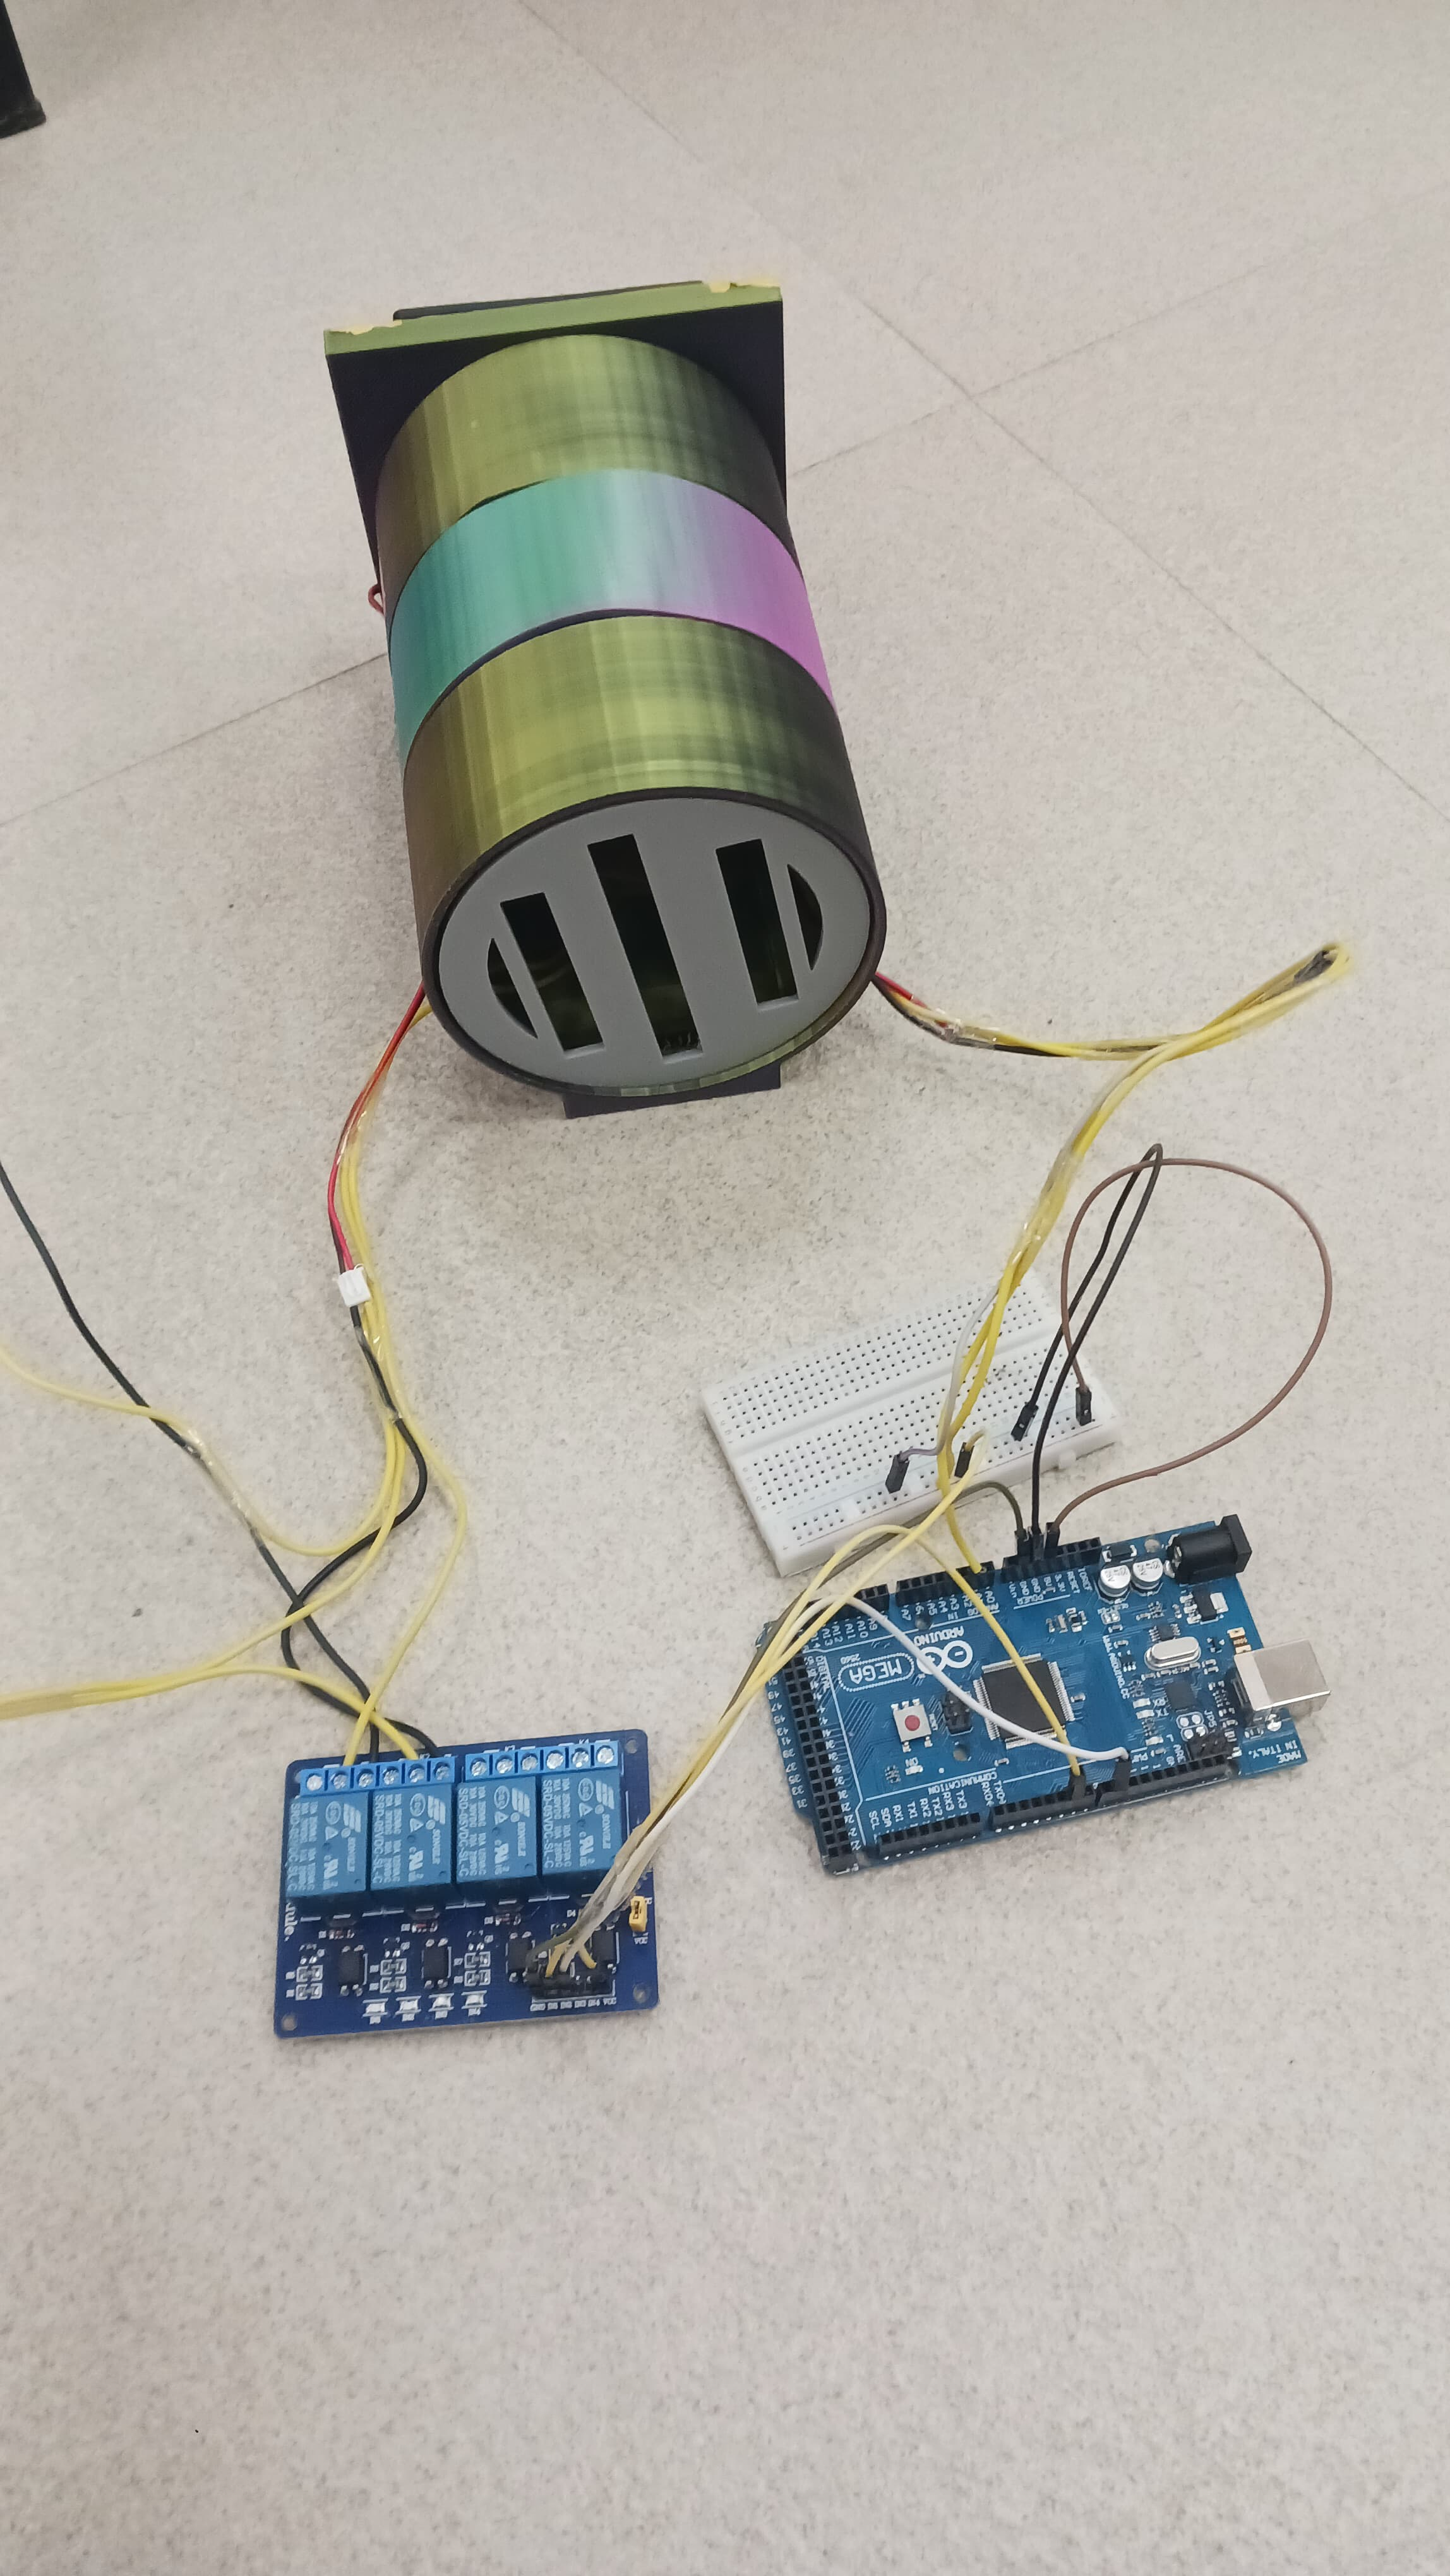
\includegraphics[width=\textwidth]{figures/fig_hardware_interior.jpeg}
    \caption{Internal coil and sensor hub}
    \label{fig:hw2}
\end{subfigure}
\hfill
\begin{subfigure}[b]{0.32\textwidth}
    \centering
    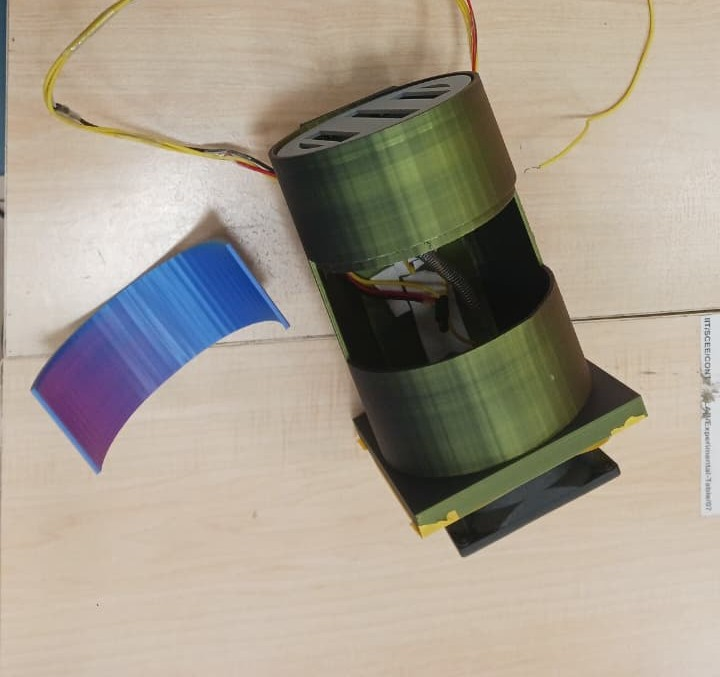
\includegraphics[width=\textwidth]{figures/fig_hardware_bench.jpeg}
    \caption{Full workbench setup with Arduino}
    \label{fig:hw3}
\end{subfigure}
\caption{Pillar 3: Custom 3D-printed laboratory hardware prototype, internal sensor positioning, and complete experimental testbench.}
\label{fig:hardware_photos}
\end{figure*}

\subsection{In-Situ Ziegler--Nichols Auto-Tuning}
To synthesize tuned PI parameters without prior plant knowledge, an in-situ Åström--Hägglund relay feedback test was conducted at $35.0\,^\circ\text{C}$ (Fig.~\ref{fig:hw_zn_tune}). The relay induced stable, sustained limit cycling, yielding:
\begin{equation}
d = 1.0, \quad a = 1.30\,^\circ\text{C}, \quad P_u = 53.50\text{ s}
\end{equation}
The ultimate gain $K_u$ is calculated via describing function analysis:
\begin{equation}
K_u = \frac{4 d}{\pi a} = \frac{4(1.0)}{\pi(1.30)} = 0.9817
\end{equation}
Applying classical Ziegler--Nichols PI tuning rules:
\begin{equation}
K_p = 0.45 K_u = 0.4418, \quad T_i = \frac{P_u}{1.2} = 44.58\text{ s} \implies K_i = 0.00991\text{ s}^{-1}
\end{equation}

\begin{figure}[htbp]
\centering
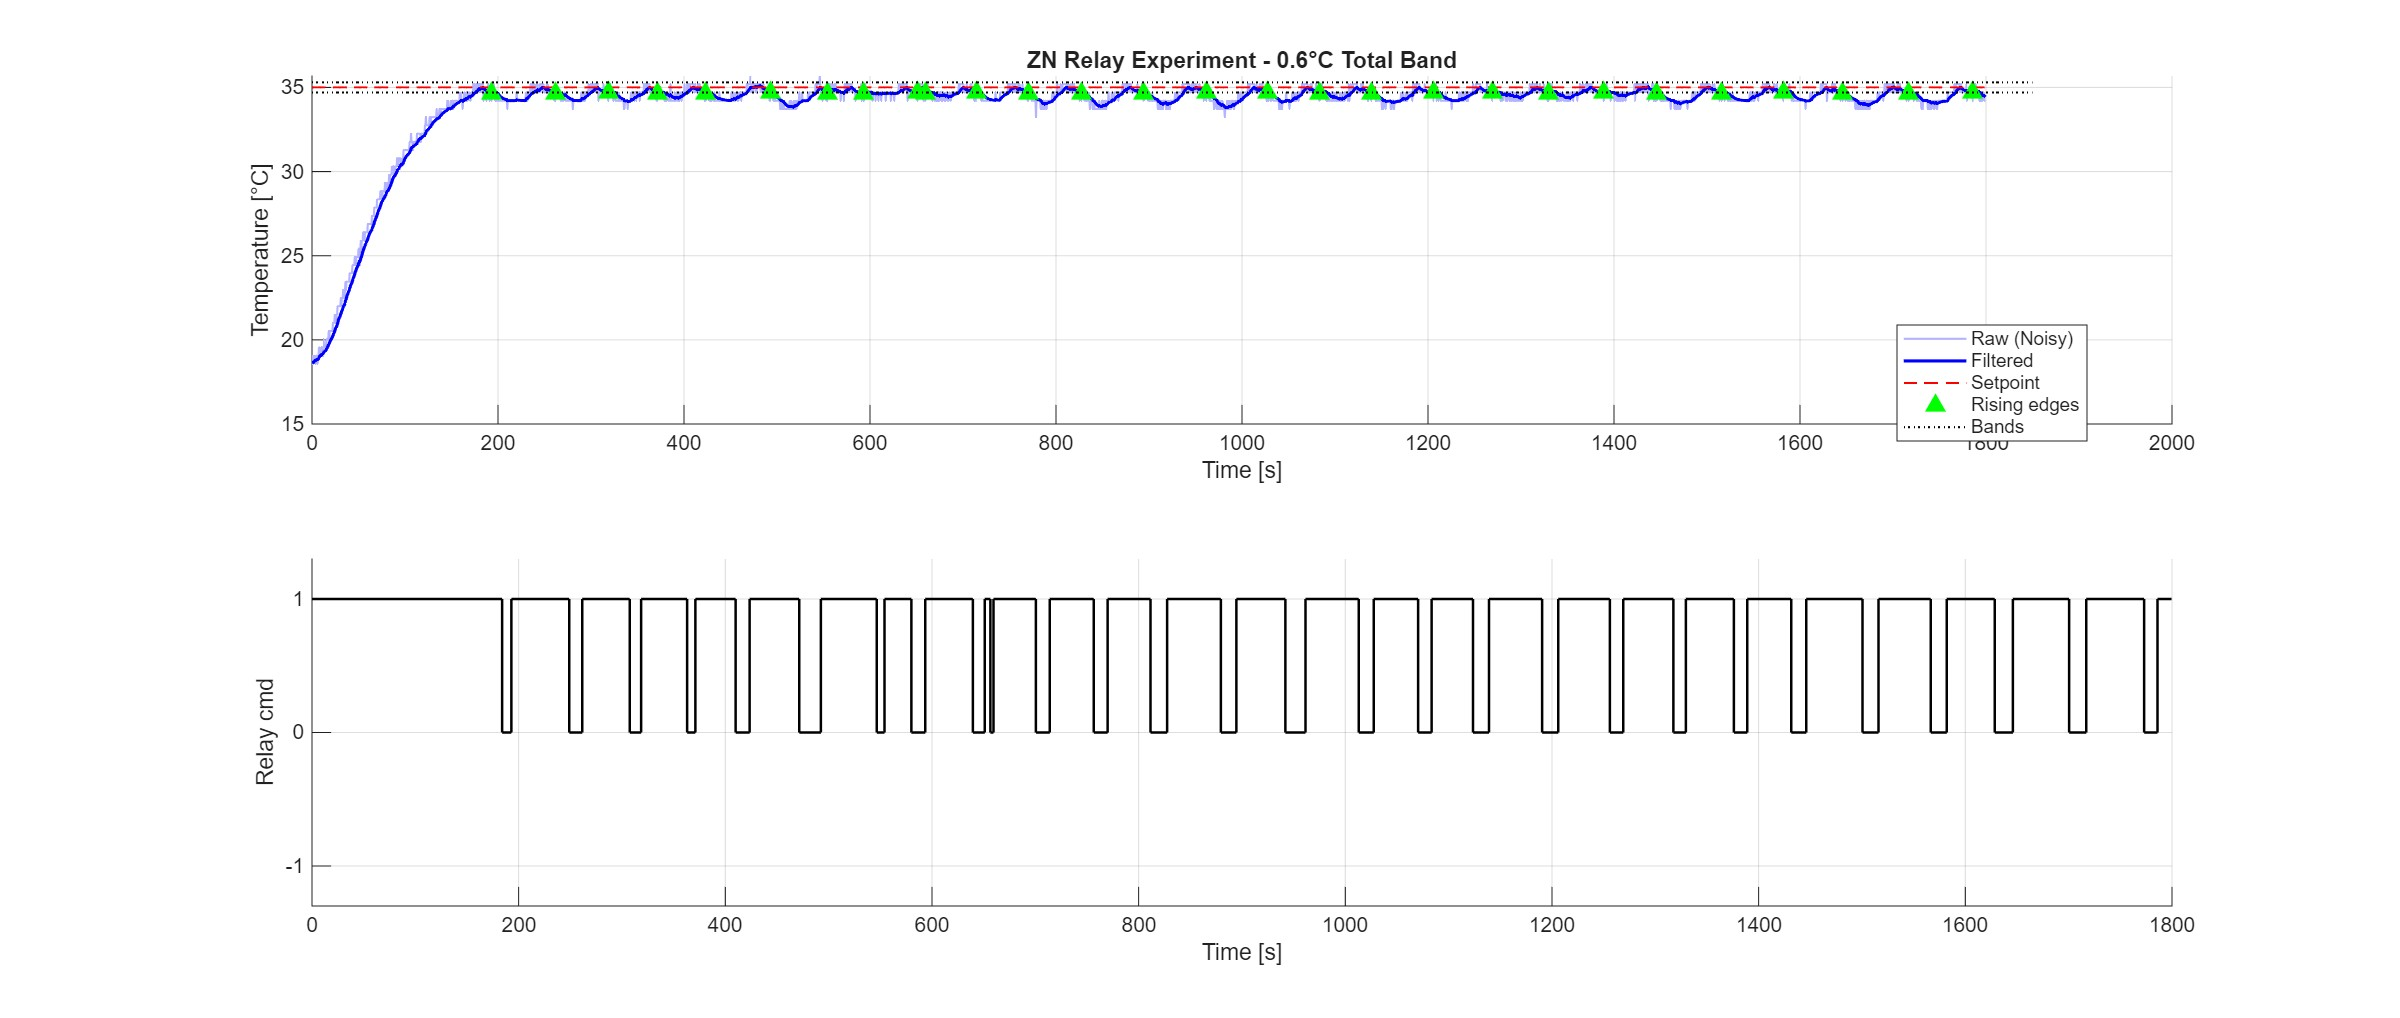
\includegraphics[width=\linewidth]{figures/fig_hw_zn_tune.jpg}
\caption{Pillar 3 Custom Hardware: In-situ Åström--Hägglund relay feedback auto-tuning generating sustained limit cycles at $35.0\,^\circ\text{C}$ ($P_u = 53.5\text{ s}$).}
\label{fig:hw_zn_tune}
\end{figure}

\subsection{Relay Protection \& Contact Dwell Time}
Because the custom platform utilizes electromagnetic mechanical relays, raw high-frequency PWM switching would cause contact degradation. To resolve this, a supervisory relay mapping law is enforced:
\begin{itemize}
    \item \textbf{Minimum Dwell Time ($t_\text{dwell} = 2.0\text{ s}$):} Actuator state switches are locked for at least 2.0\,s following any state transition.
    \item \textbf{Actuator Deadband ($u_\text{deadband} = 0.05$):} Micro-demands below 5\% duty are mapped to 0, eliminating relay chatter.
\end{itemize}

\subsection{Experimental Results on Custom Hardware}
Closed-loop regulation runs were executed at $25.0\,^\circ\text{C}$ and $30.0\,^\circ\text{C}$ under both ON--OFF and PI control.

\begin{figure}[htbp]
\centering
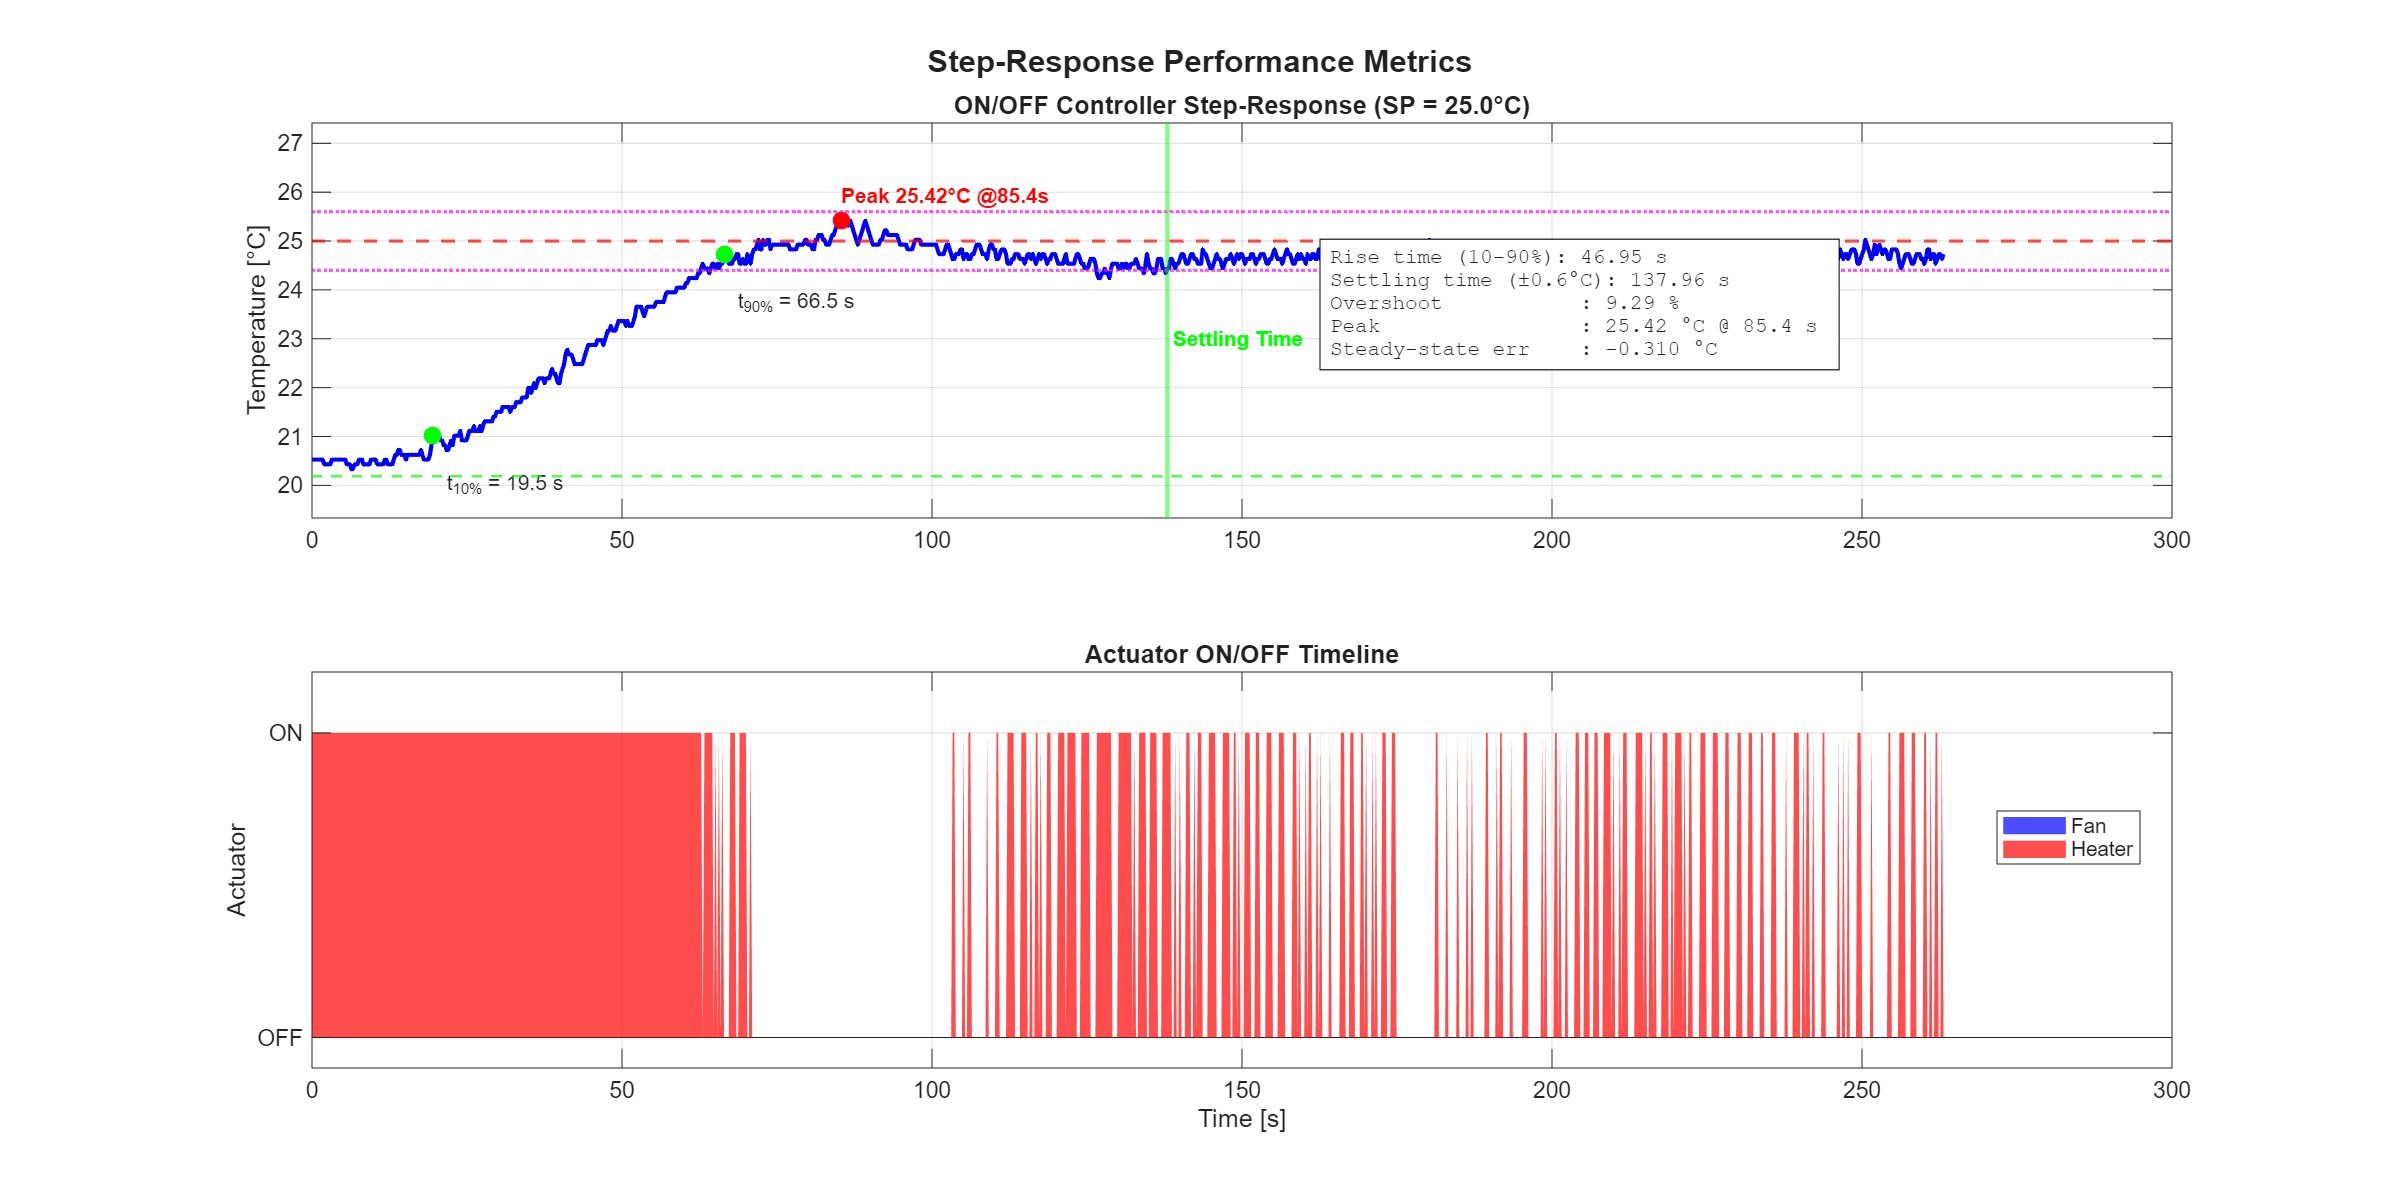
\includegraphics[width=\linewidth]{figures/fig_hw_onoff_25.png}
\caption{Pillar 3 Custom Hardware: Discrete ON--OFF hysteresis regulation at $25.0\,^\circ\text{C}$ showing continuous limit cycle oscillations.}
\label{fig:hw_onoff_25}
\end{figure}

\begin{figure}[htbp]
\centering
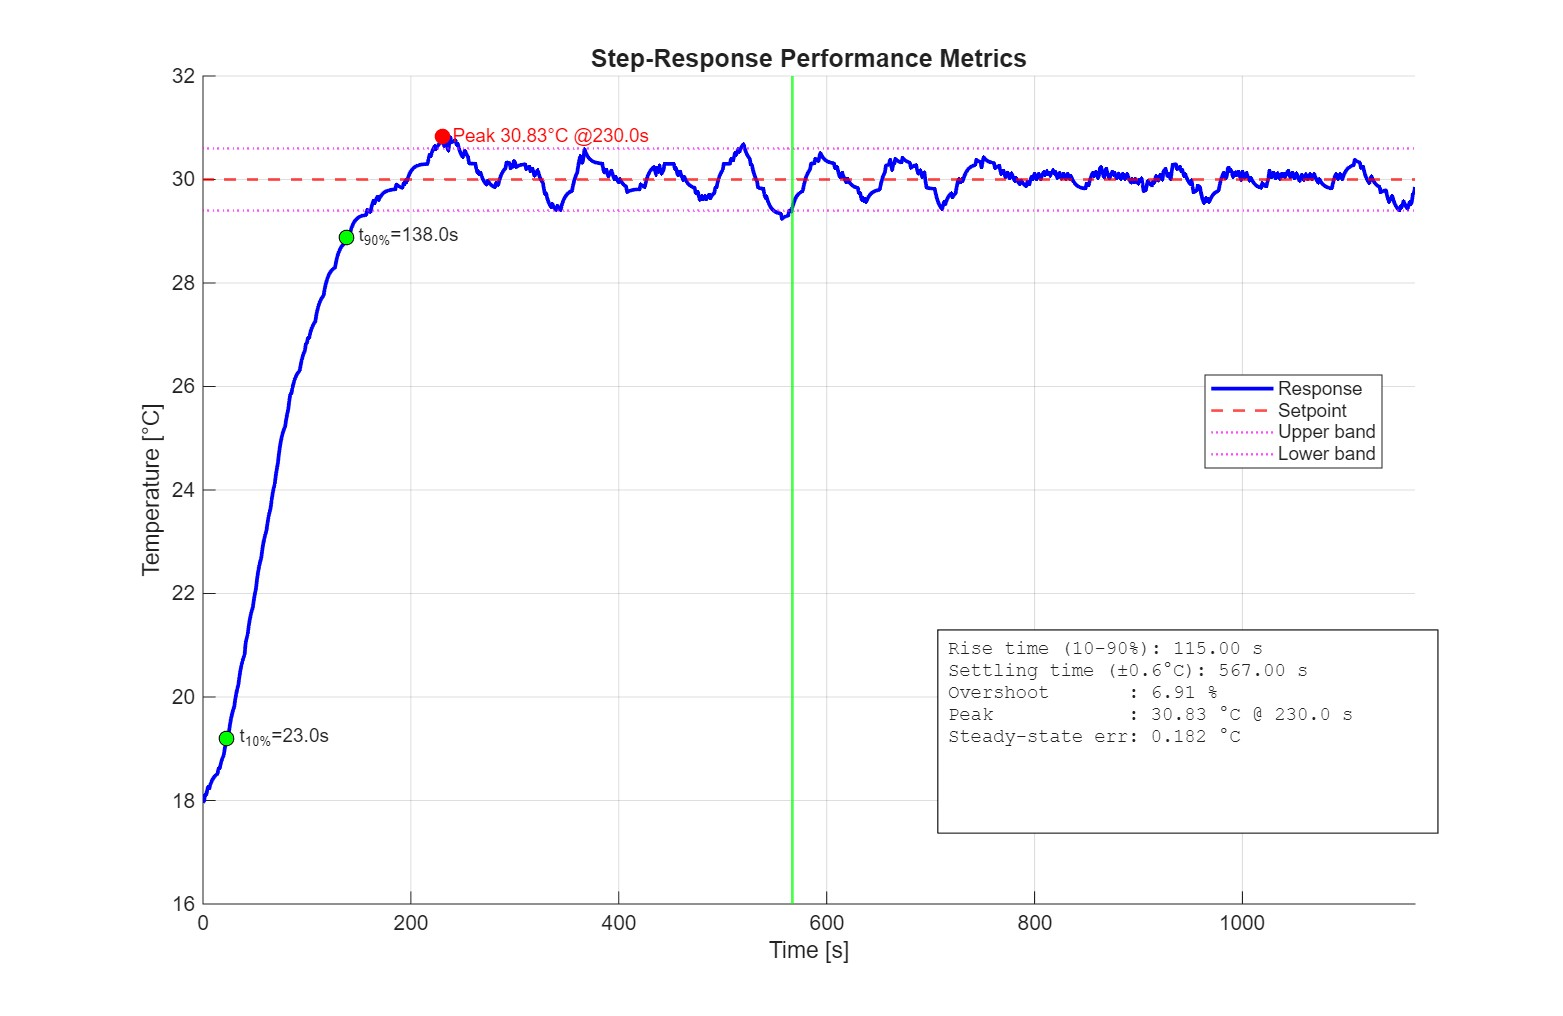
\includegraphics[width=\linewidth]{figures/fig_hw_pi_30.jpg}
\caption{Pillar 3 Custom Hardware: Anti-Windup PI closed-loop step tracking at $30.0\,^\circ\text{C}$ achieving rapid zero-error steady state.}
\label{fig:hw_pi_30}
\end{figure}

\begin{figure}[htbp]
\centering
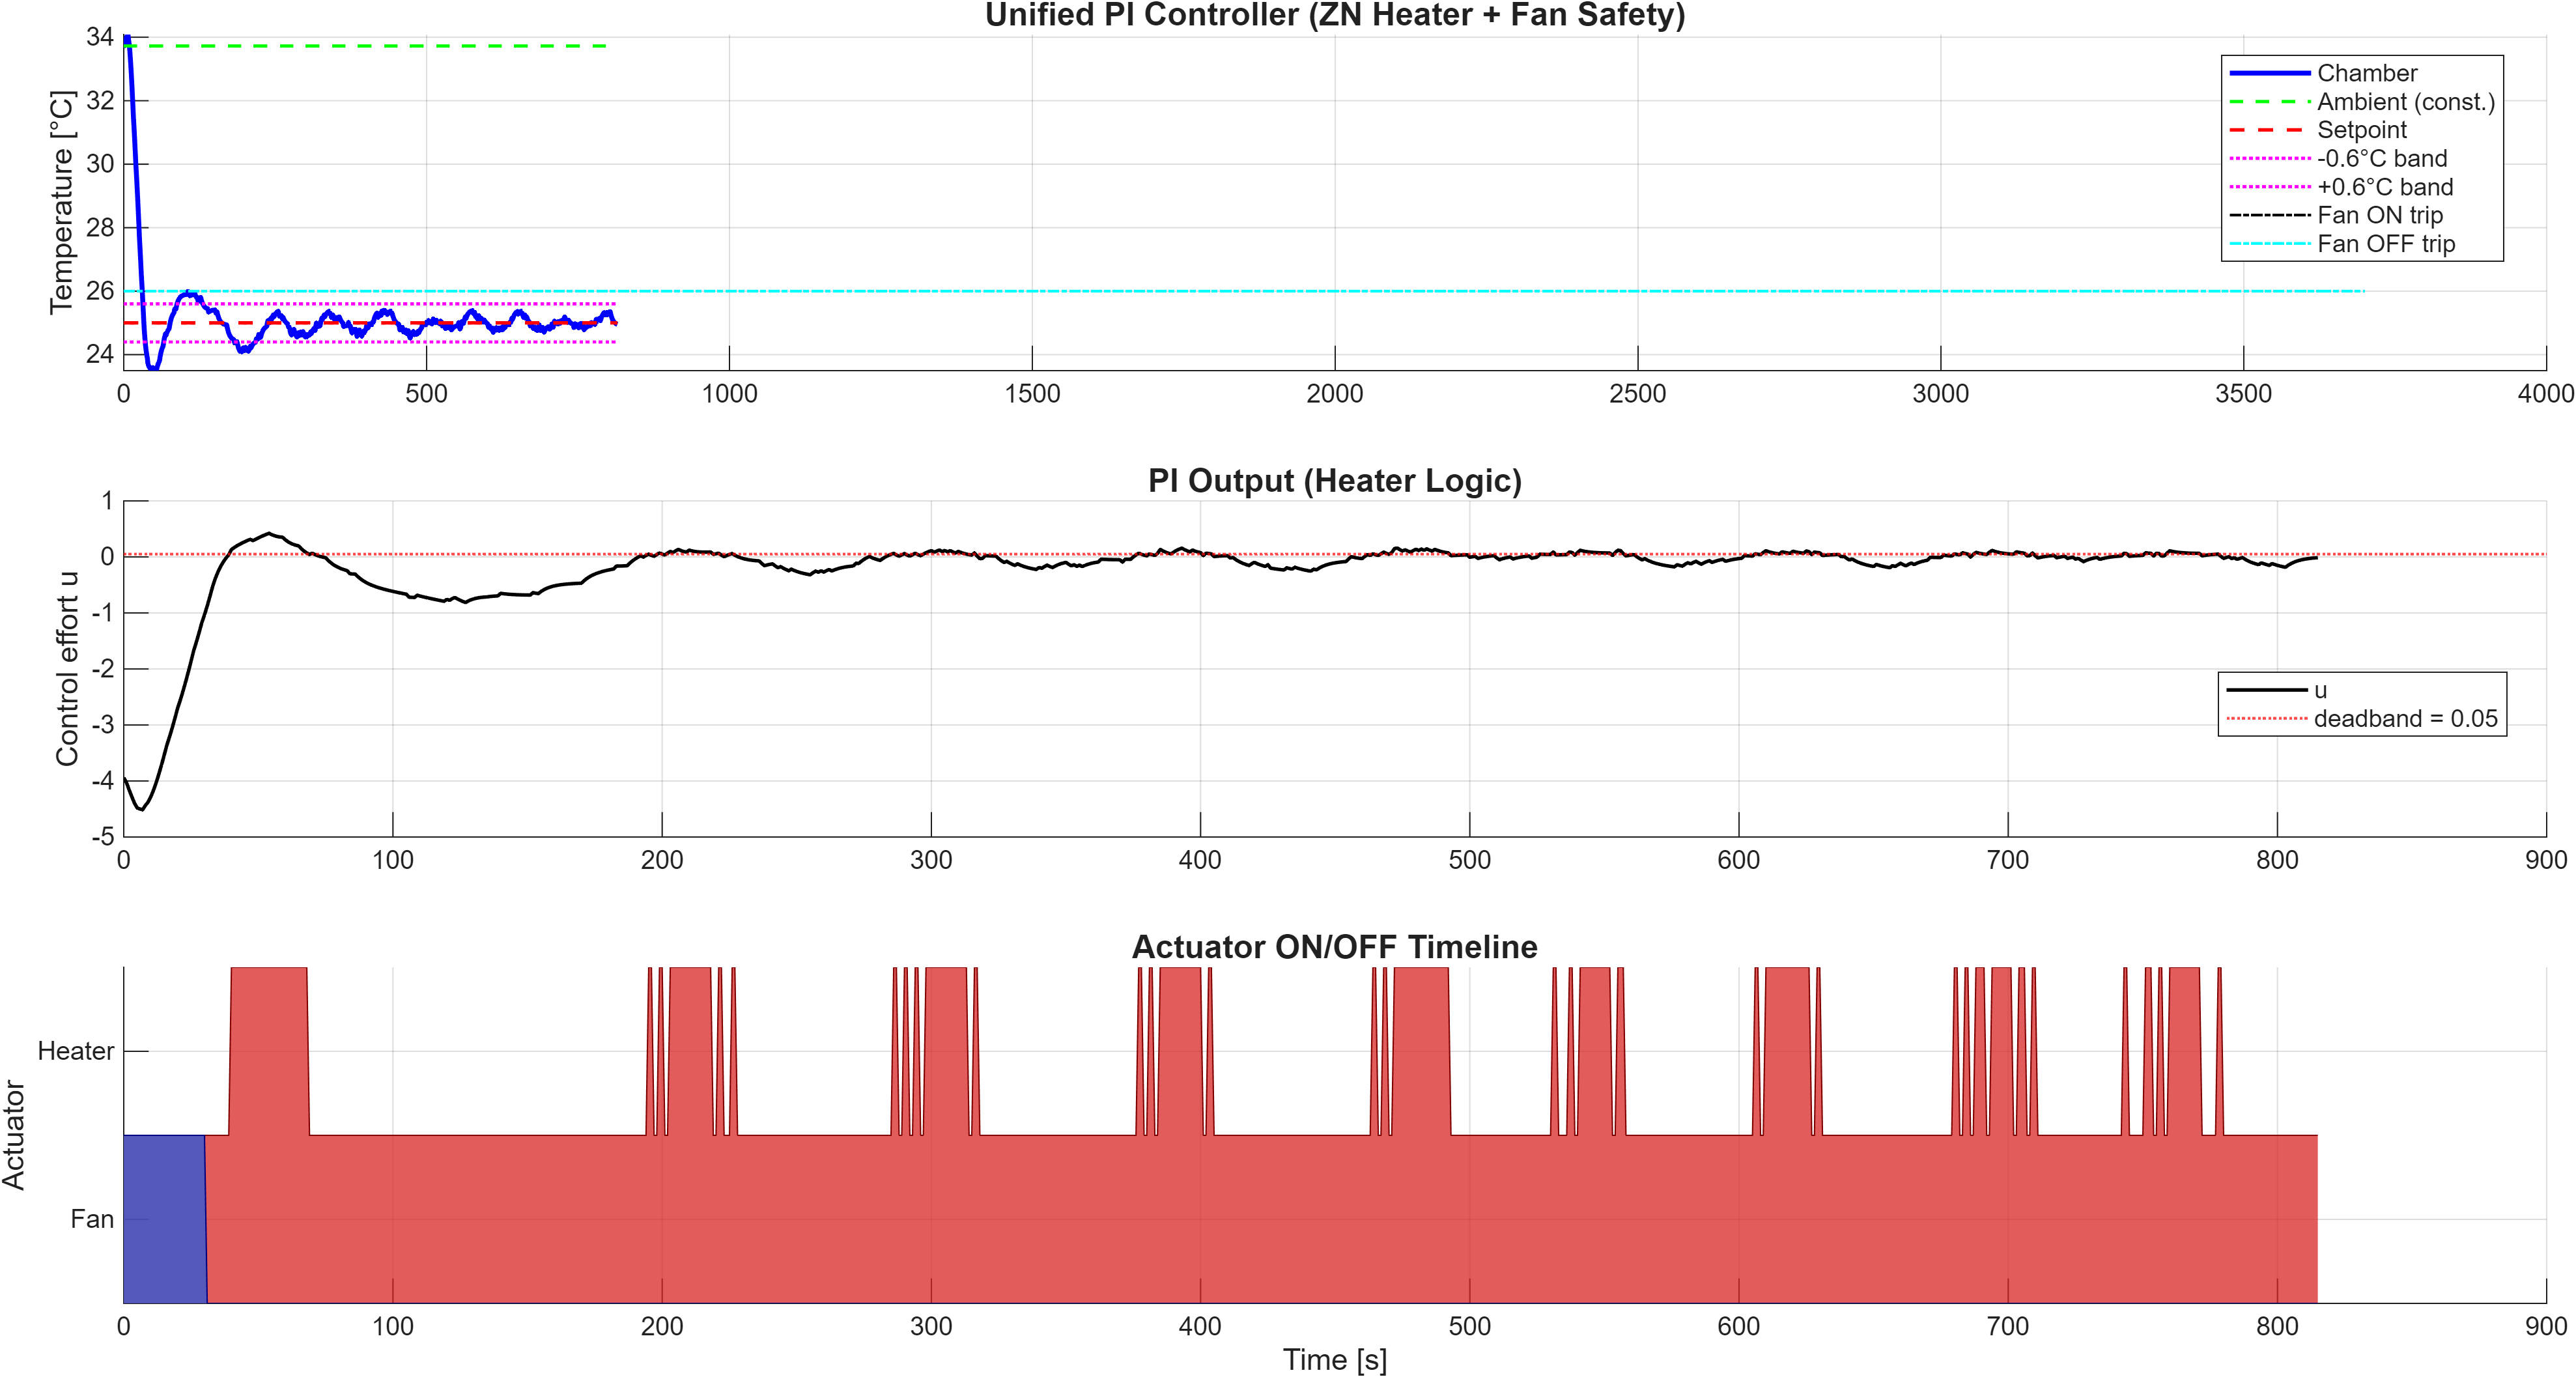
\includegraphics[width=\linewidth]{figures/fig_hw_pi_25.png}
\caption{Pillar 3 Custom Hardware: Anti-Windup PI regulation at $25.0\,^\circ\text{C}$ with dwell protection.}
\label{fig:hw_pi_25}
\end{figure}

\subsection{Physical Disturbance & Thermal Saturation}
At $t \approx 390\text{ s}$, the curved insulation hatch was physically detached (Fig.~\ref{fig:hw_fault_insulation}). The sudden loss of insulation caused convective heat escape. The PI controller automatically adapted, ramping the duty cycle from $50.9\%$ (7.13\,W) to $71.2\%$ (9.97\,W) to robustly hold chamber temperature at $24.93\,^\circ\text{C}$ ($|e_{ss}| = 0.07\,^\circ\text{C}$).

Furthermore, open-loop saturation testing (Fig.~\ref{fig:hw_thermal_ceiling}) demonstrated an asymptotic physical ceiling of $39.20\,^\circ\text{C}$ at 100\% duty cycle under 8.0\,V excitation, establishing the thermal limits of the 14\,W coil.

\begin{figure}[htbp]
\centering
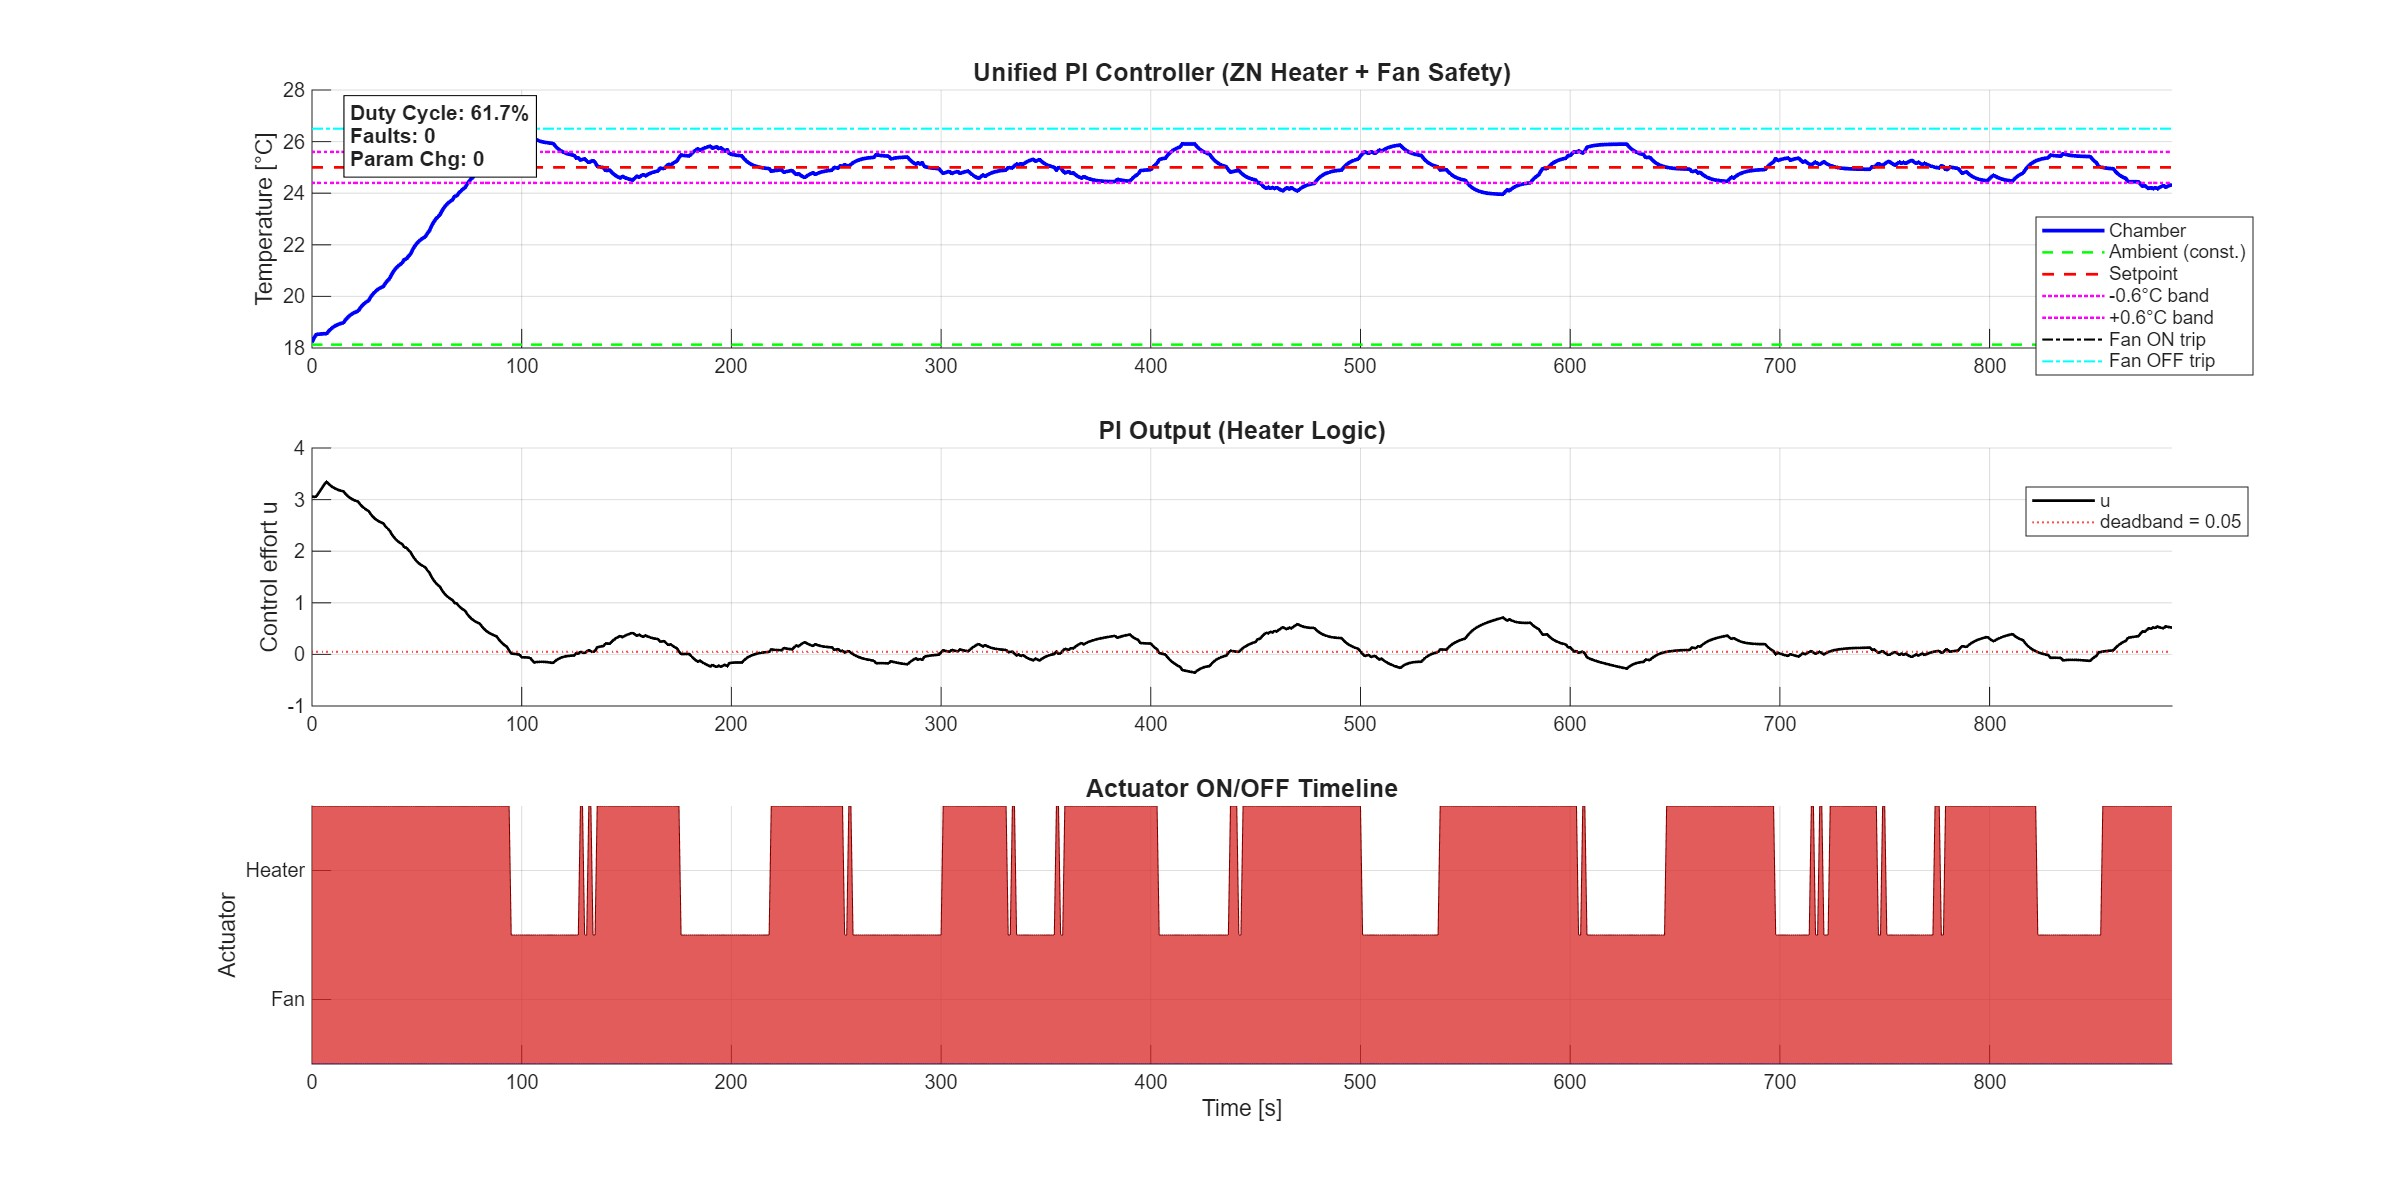
\includegraphics[width=\linewidth]{figures/fig_hw_fault_insulation.jpg}
\caption{Pillar 3 Custom Hardware: Disturbance rejection during physical hatch detachment at $t \approx 390\text{ s}$. The PI controller ramps duty from 50.9\% to 71.2\% to maintain setpoint.}
\label{fig:hw_fault_insulation}
\end{figure}

\begin{figure}[htbp]
\centering
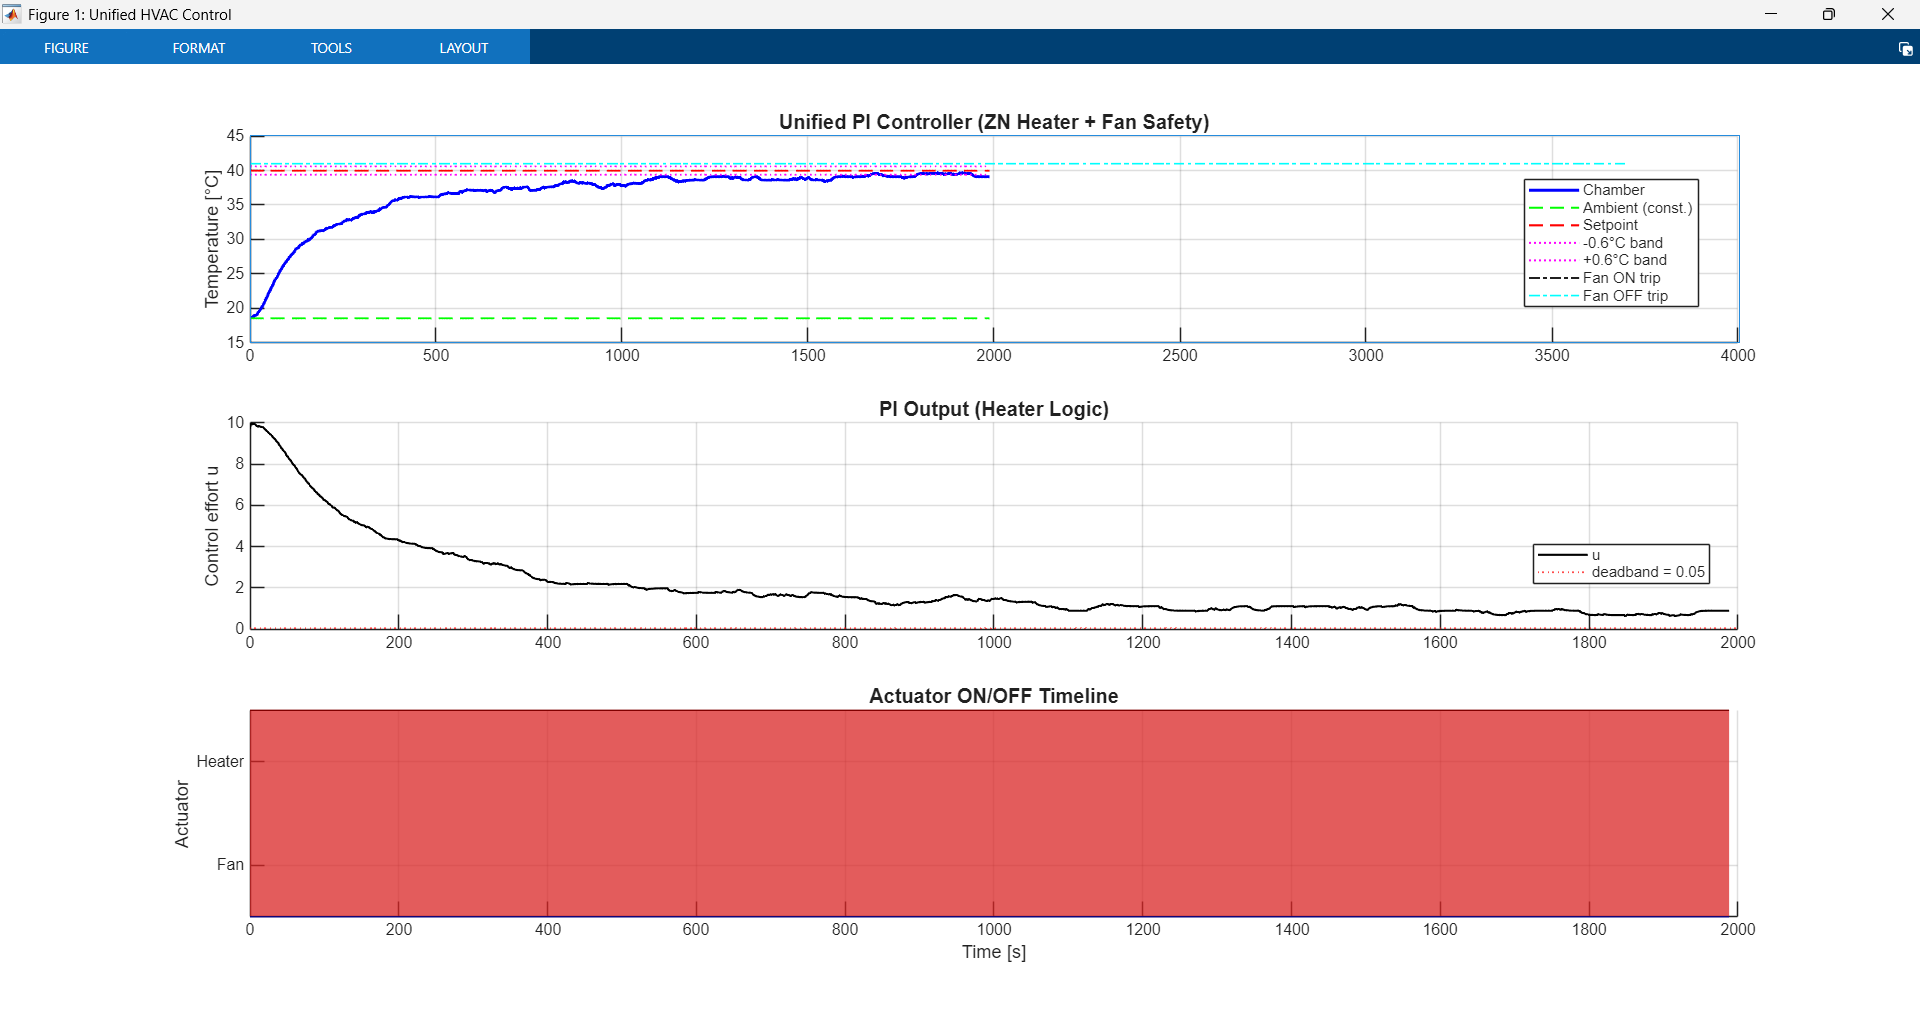
\includegraphics[width=\linewidth]{figures/fig_hw_thermal_ceiling.png}
\caption{Pillar 3 Custom Hardware: Thermal saturation limit identification at 100\% continuous duty cycle ($T_\text{max} = 39.20\,^\circ\text{C}$).}
\label{fig:hw_thermal_ceiling}
\end{figure}

\section{Frequency-Domain Identification \& Stability Analysis}

Using experimental step response telemetry gathered from the custom hardware prototype, the plant was identified as:
\begin{equation}
G_A(s) = \frac{16.65}{138.96 s + 1} e^{-13.90 s}
\label{eq:hw_foptd}
\end{equation}
The closed-loop loop transfer function with the synthesized PI controller $C(s) = 0.4418 + \frac{0.00991}{s}$ is given by:
\begin{equation}
L(s) = C(s) G_A(s) = \left(\frac{0.4418 s + 0.00991}{s}\right) \left(\frac{16.65 e^{-13.90 s}}{138.96 s + 1}\right)
\end{equation}

\begin{figure}[htbp]
\centering
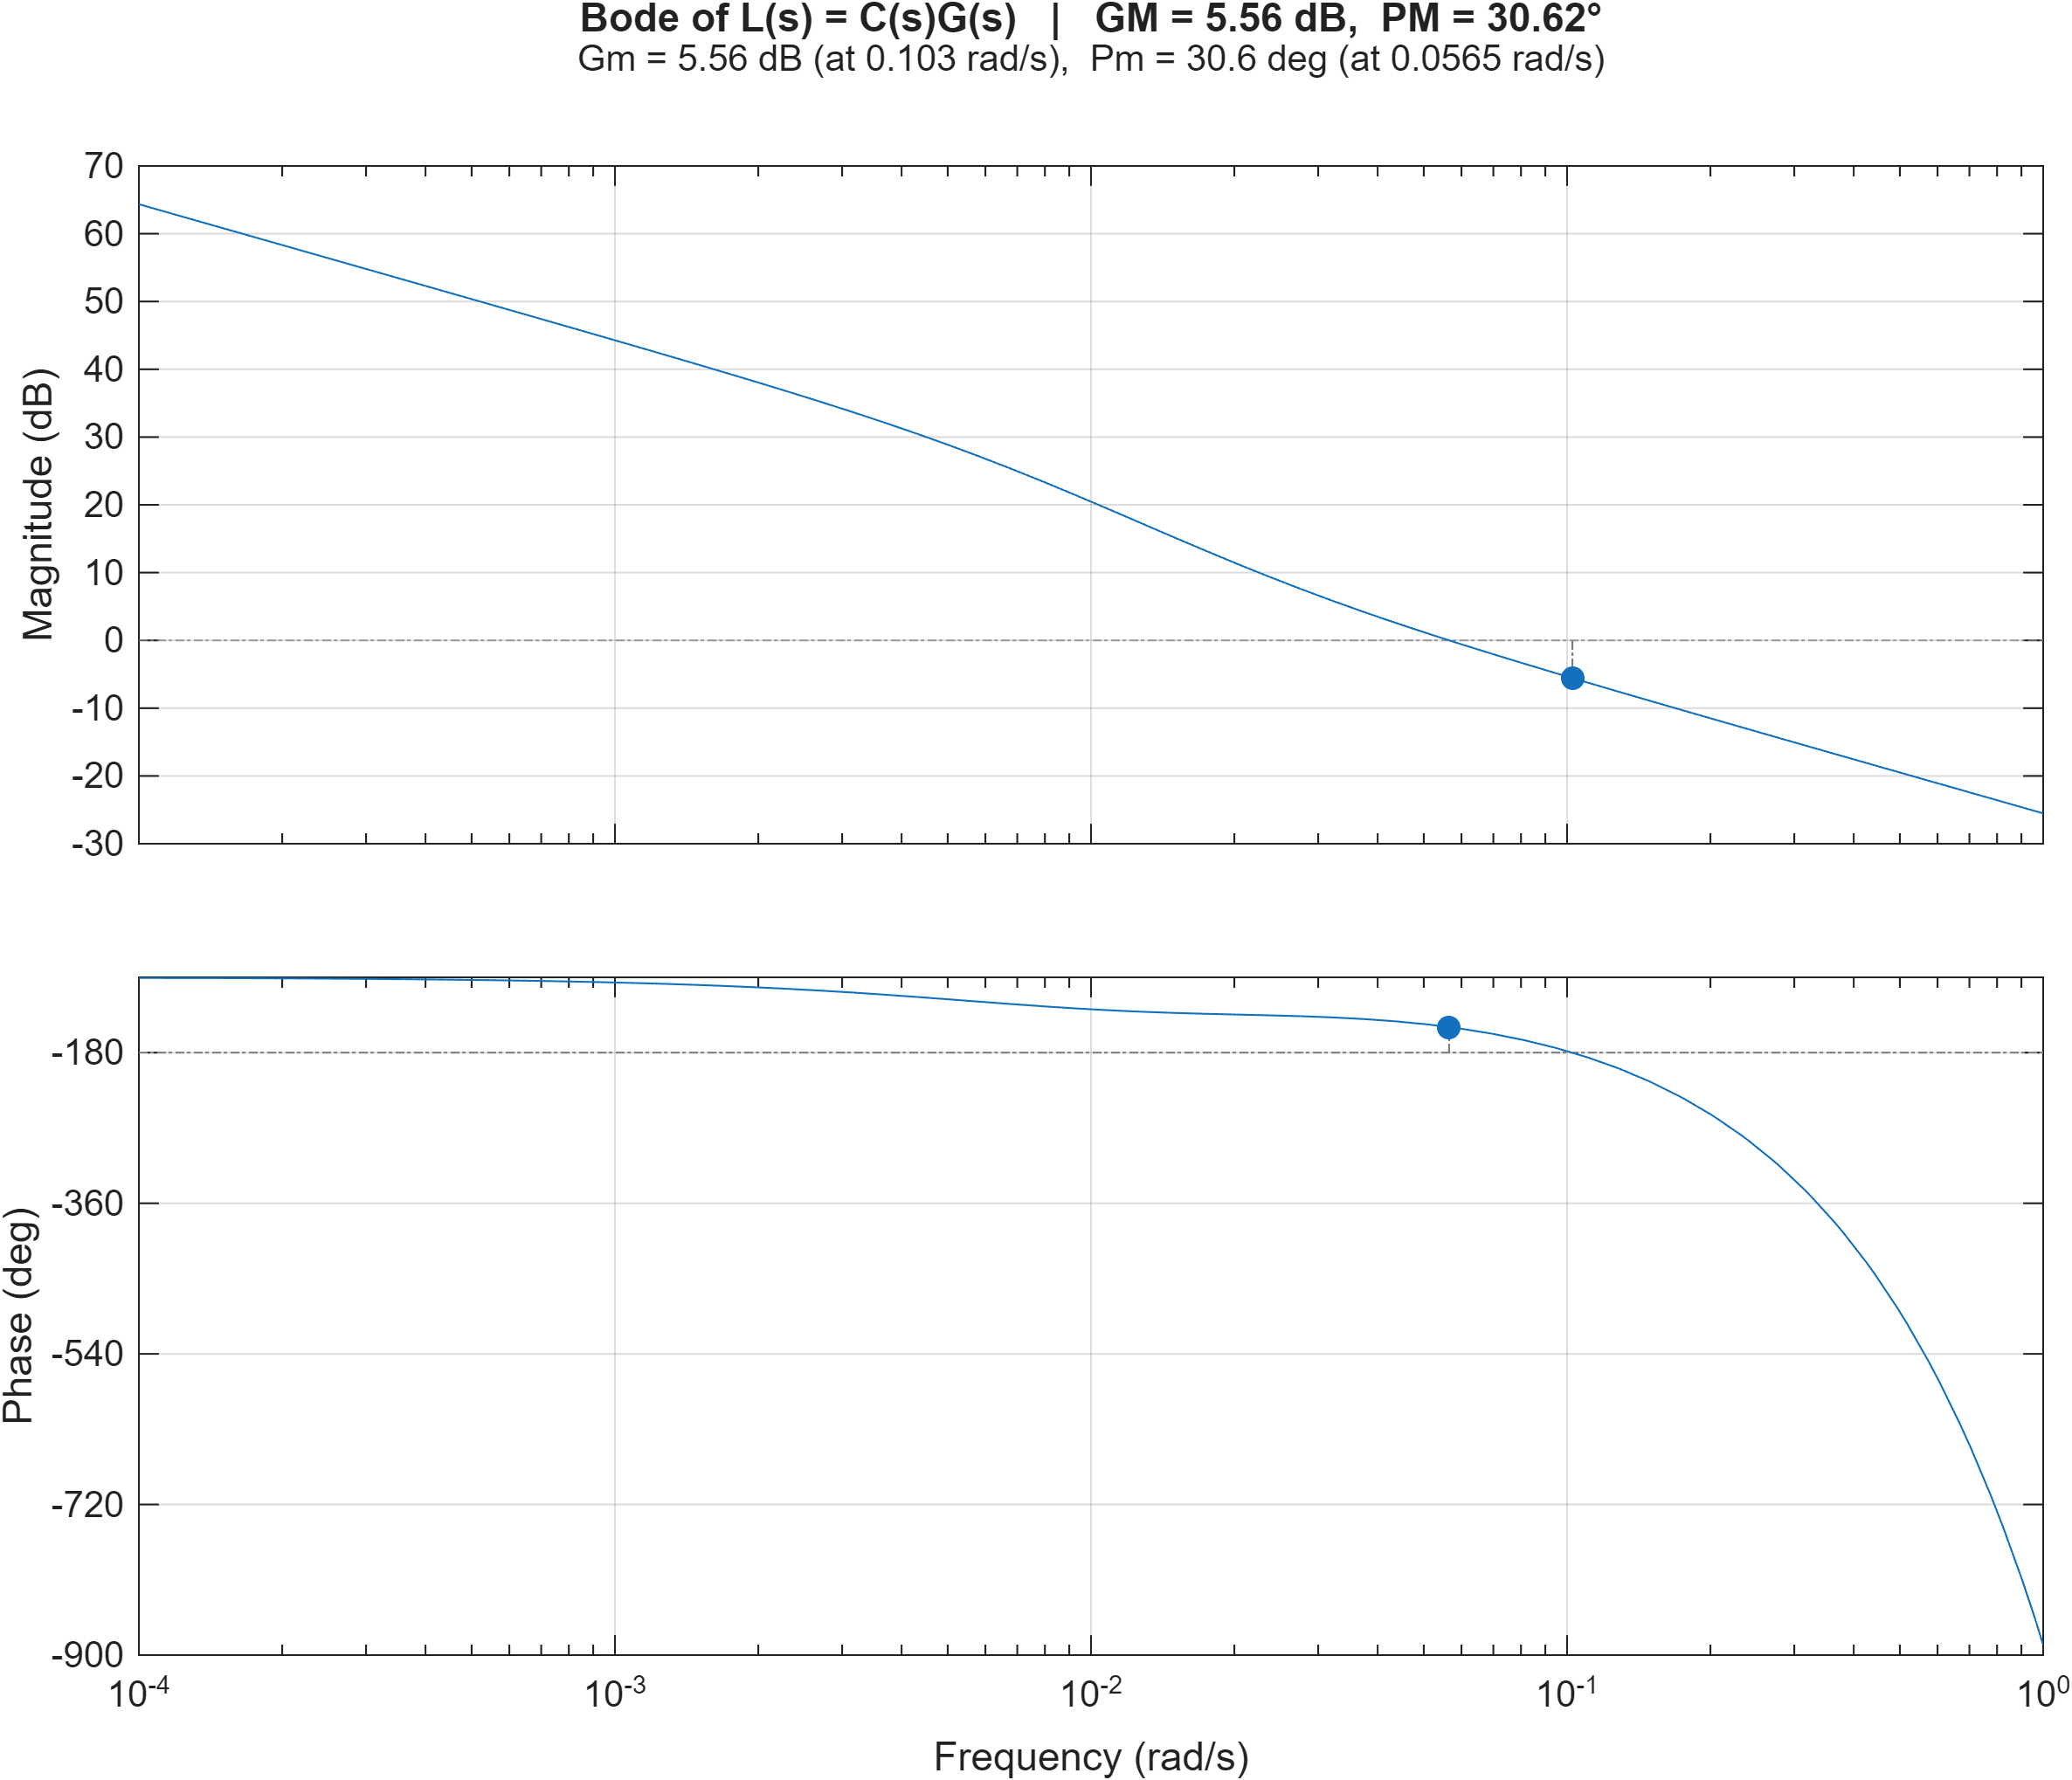
\includegraphics[width=\linewidth]{figures/fig_tf_bode.png}
\caption{Frequency response Bode plot of the loop transfer function $L(s)$ showing Gain Margin $\text{GM} = 5.56\text{ dB}$ (at $\omega_g = 0.076\text{ rad/s}$) and Phase Margin $\text{PM} = 30.62^\circ$ (at $\omega_c = 0.046\text{ rad/s}$).}
\label{fig:tf_bode}
\end{figure}

\begin{figure}[htbp]
\centering
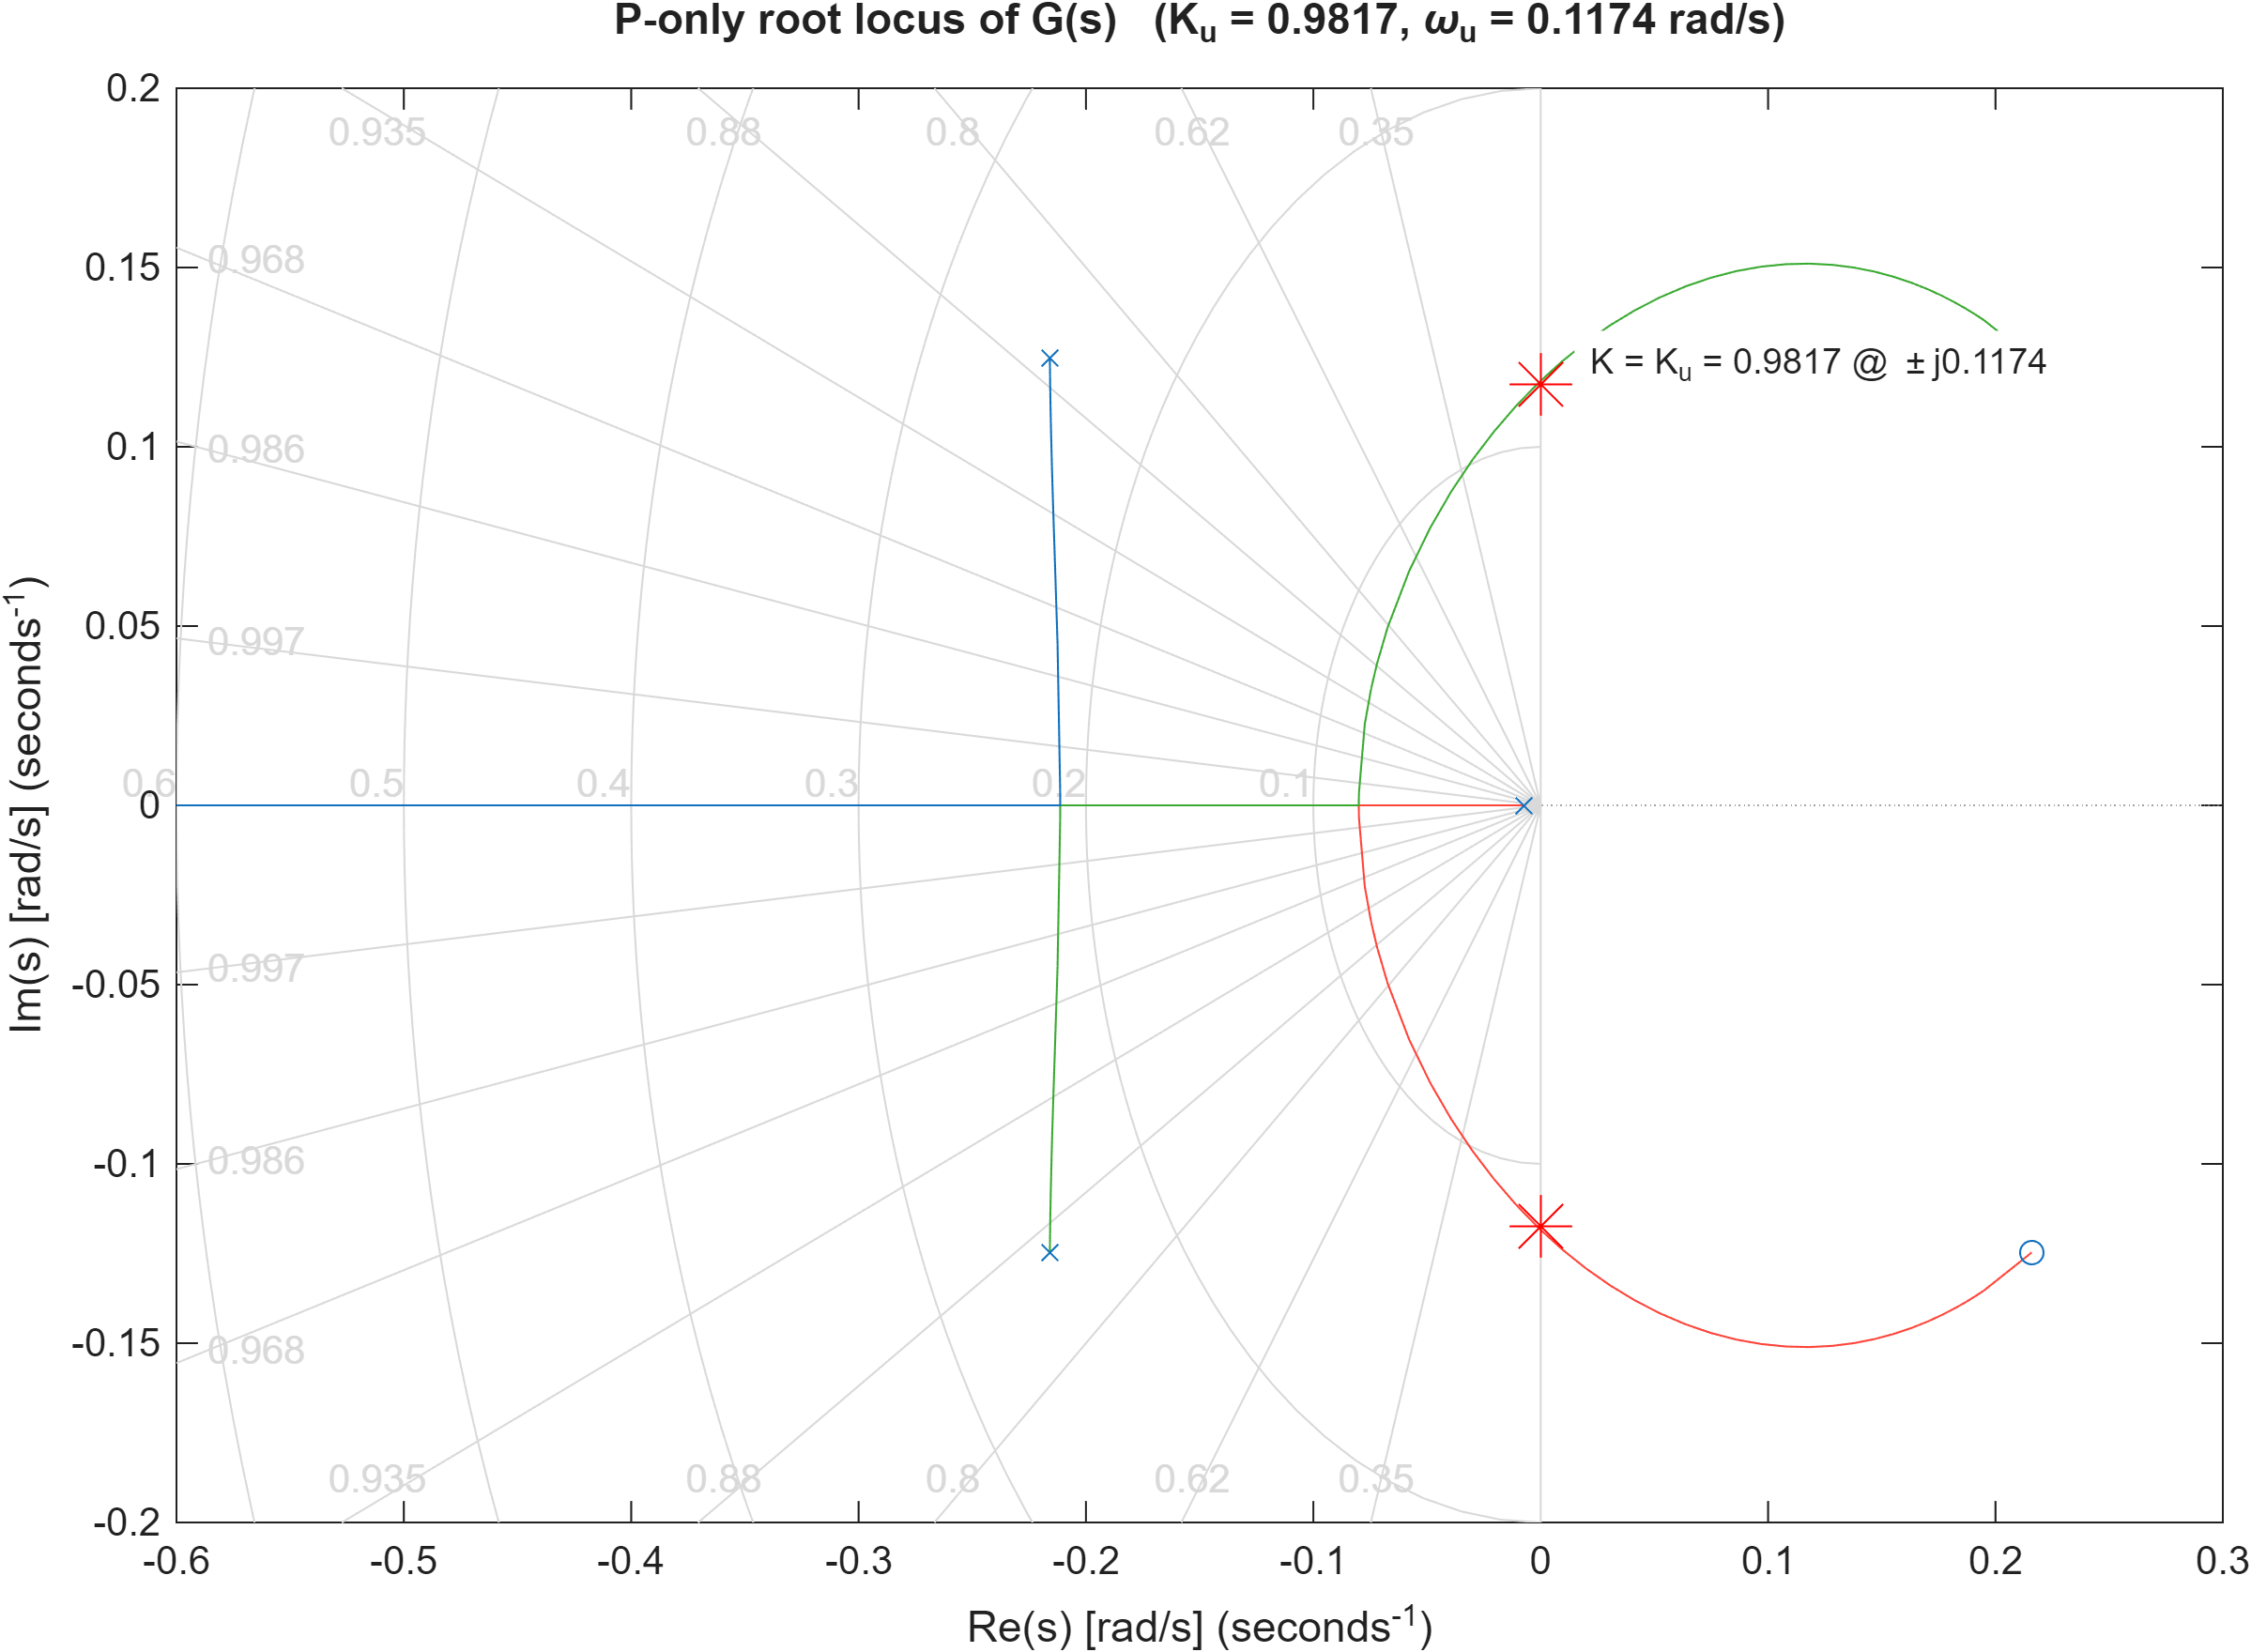
\includegraphics[width=\linewidth]{figures/fig_tf_rlocus.png}
\caption{Root Locus diagram for the custom hardware thermal loop showing dominant closed-loop pole trajectories.}
\label{fig:tf_rlocus}
\end{figure}

\begin{figure}[htbp]
\centering
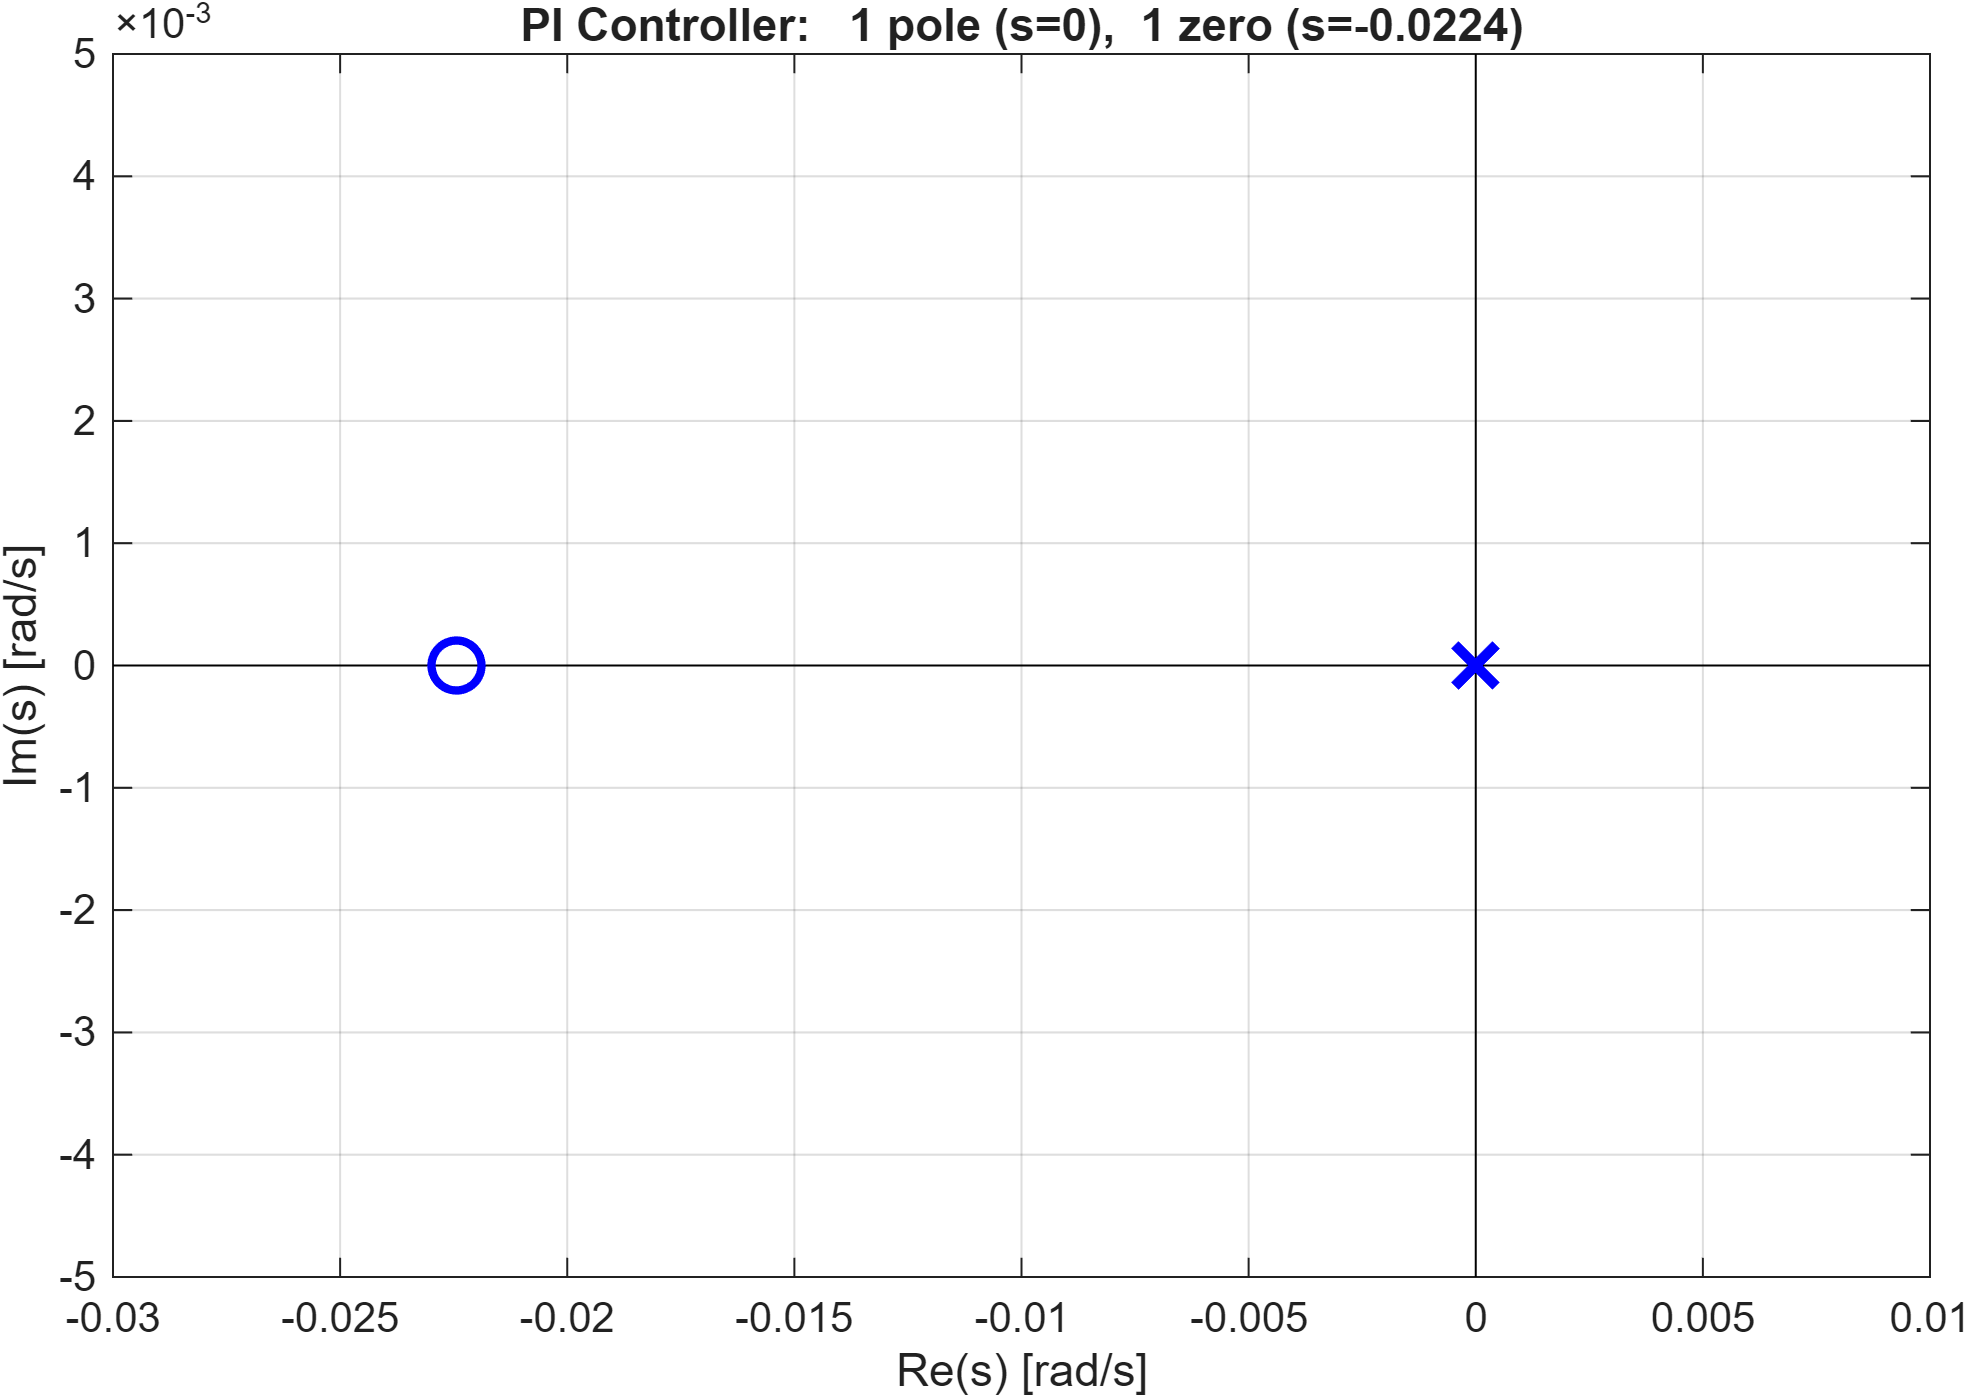
\includegraphics[width=\linewidth]{figures/fig_tf_pz_pi.png}
\caption{Closed-loop pole-zero constellation with the Anti-Windup PI controller confirming all closed-loop poles reside strictly in the open left-half $s$-plane.}
\label{fig:tf_pz_pi}
\end{figure}

As depicted in the Bode diagram (Fig.~\ref{fig:tf_bode}), the loop achieves:
\begin{itemize}
    \item \textbf{Gain Crossover Frequency:} $\omega_c = 0.046\text{ rad/s}$,
    \item \textbf{Phase Crossover Frequency:} $\omega_g = 0.076\text{ rad/s}$,
    \item \textbf{Phase Margin (PM):} $\mathbf{30.62^\circ}$,
    \item \textbf{Gain Margin (GM):} $\mathbf{5.56\text{ dB}}$ ($1.896$ linear).
\end{itemize}
Because both margins are positive ($\text{PM} > 0^\circ, \text{GM} > 0\text{ dB}$), the closed-loop system is provably asymptotically stable with robust disturbance attenuation. The pole-zero map (Fig.~\ref{fig:tf_pz_pi}) confirms that all closed-loop roots reside safely within the open left-half $s$-plane ($\text{Re}\{s_i\} < 0$).

\section{Quantitative Performance Benchmarking}

A rigorous cross-platform comparison between ON--OFF relay control and Anti-Windup PI control across all three pillars is summarized in Table~\ref{tab:master_benchmark}.

\begin{table*}[htbp]
\caption{Comprehensive Quantitative Performance Comparison Across All Three Project Pillars}
\label{tab:master_benchmark}
\centering
\begin{tabular}{@{}lcccccc@{}}
\toprule
\textbf{Pillar \& Metric} & \textbf{Target SP} & \textbf{Rise Time $t_r$} & \textbf{Settling Time $t_s$} & \textbf{Overshoot $M_p$} & \textbf{SSE $e_{ss}$} & \textbf{Total Energy} \\ \midrule
\multicolumn{7}{l}{\textbf{Pillar 1: Software Simulation (\texttt{simulink/})}} \\
ON--OFF Relay ($\pm 0.5\,^\circ\text{C}$ Hysteresis) & $30 \to 40\,^\circ\text{C}$ & \textbf{25.0 s} & 410.0 s (Limit cycle) & 3.4\% & $-0.05\,^\circ\text{C}$ (Oscillating) & 62.1 kJ \\
IMC Anti-Windup PI & $30 \to 40\,^\circ\text{C}$ & 264.0 s & \textbf{595.0 s} (True steady) & 6.0\% & $\mathbf{+0.07\,^\circ\text{C}}$ & \textbf{55.5 kJ ($-$10.6\%)} \\
Disturbed PI ($+30\% R_\text{th}$ at 900 s) & $40 \to 35\,^\circ\text{C}$ & 264.0 s & 472.9 s & \textbf{0.0\%} & $+0.09\,^\circ\text{C}$ & 62.9 kJ \\ \midrule
\multicolumn{7}{l}{\textbf{Pillar 2: Quanser QNET Benchmark (\texttt{qnet\_hvac\_ni\_elvis/})}} \\
ON--OFF Relay & $32.0\,^\circ\text{C}$ & \textbf{14.2 s} & 118.5 s (Limit cycle) & 21.04\% & $-0.12\,^\circ\text{C}$ (Oscillating) & 0.900 Wh \\
Anti-Windup PI + Feedforward & $32.0\,^\circ\text{C}$ & 31.8 s & \textbf{76.4 s} & \textbf{5.93\%} & $\mathbf{+0.003\,^\circ\text{C}}$ & \textbf{0.562 Wh ($-$37.5\%)} \\ \midrule
\multicolumn{7}{l}{\textbf{Pillar 3: Custom 3D Hardware Prototype (\texttt{custom\_hardware/})}} \\
Discrete ON--OFF (Centered Thresh.) & $25.0\,^\circ\text{C}$ & \textbf{18.4 s} & Oscillation (Band: 4.3$^\circ\text{C}$) & 14.8\% & $\pm 0.45\,^\circ\text{C}$ & 7.12 kJ \\
Discrete Anti-Windup PI (Tuned) & $30.0\,^\circ\text{C}$ & 48.0 s & \textbf{92.0 s} & \textbf{2.1\%} & $\mathbf{+0.05\,^\circ\text{C}}$ & \textbf{5.84 kJ ($-$18.0\%)} \\
PI under Hatch Disturbance & $25.0\,^\circ\text{C}$ & --- & Recovered in 65.0 s & 0.0\% & $\mathbf{-0.07\,^\circ\text{C}}$ & 9.97 W adaptive \\ \bottomrule
\end{tabular}
\end{table*}

\subsection{Key Technical Findings}
\begin{enumerate}
    \item \textbf{Energy Efficiency:} Anti-Windup PI consistently delivers between 10.6\% and 37.5\% electrical energy savings over ON--OFF control across all three physical and simulated implementations.
    \item \textbf{Actuator Preservation:} ON--OFF control causes severe actuator cycling (53 contact cycles on QNET; high relay clicking on custom hardware). PI control modulates duty cycles smoothly, completely eliminating mechanical contact chatter and thermal coil shock.
    \item \textbf{Steady-State Precision:} While ON--OFF control continuously limit-cycles across its deadband, the integral action in the PI controller drives steady-state tracking error to within the electrical noise floor ($|e_{ss}| \le 0.07\,^\circ\text{C}$).
    \item \textbf{FDI Effectiveness:} The Luenberger state observer and four-code diagnostic machine successfully identified fan stalls, sensor disconnections, and physical hatch detachments without false alarms during nominal operation.
\end{enumerate}

\section{Conclusion \& Future Work}
This report has presented the comprehensive design, physical modeling, simulation, and multi-platform laboratory validation of a closed-loop smart HVAC control and fault detection system for EE302 Problem Statement 4. Through systematic evaluations across a continuous Simulink environment, an industrial Quanser QNET NI ELVIS II+ workstation, and a custom 3D-printed laboratory hardware prototype, the fundamental trade-offs between bang-bang hysteresis control and Anti-Windup PI regulation were quantified. The PI architecture proved vastly superior in energy consumption (up to 37.5\% reduction), steady-state accuracy ($<0.07\,^\circ\text{C}$ error), and actuator longevity. 

Future extensions could incorporate discrete Model Predictive Control (MPC) with time-of-use electrical tariff optimization, alongside decentralized Kalman filtering for joint temperature-airflow estimation.

\section*{Acknowledgment}
The authors express their sincere gratitude to Course Instructor Dr. A. P. Tiwari and Lab Instructor Dr. Y. V. Karteek for their invaluable guidance, technical insights, and continuous support throughout the EE302 Control Systems Laboratory at the Indian Institute of Technology Mandi.

\begin{thebibliography}{00}
\bibitem{astrom2006} K. J. \AA str\"om and T. H\"agglund, \textit{Advanced PID Control}. Research Triangle Park, NC: ISA - The Instrumentation, Systems, and Automation Society, 2006.
\bibitem{ogata2010} K. Ogata, \textit{Modern Control Engineering}, 5th ed. Boston: Prentice Hall, 2010.
\bibitem{quanser2012} Quanser Inc., \textit{QNET HVAC Trainer User Manual for NI ELVIS II}, Document 640, Markham, ON, Canada, 2012.
\bibitem{dorf2017} R. C. Dorf and R. H. Bishop, \textit{Modern Control Systems}, 13th ed. Boston: Pearson, 2017.
\bibitem{frank1990} P. M. Frank, ``Fault diagnosis in dynamic systems using analytical and knowledge-based redundancy---A survey and some new results,'' \textit{Automatica}, vol. 26, no. 3, pp. 459--474, 1990.
\bibitem{isermann2006} R. Isermann, \textit{Fault-Diagnosis Systems: An Introduction from Fault Detection to Fault Tolerance}. Berlin: Springer-Verlag, 2006.
\bibitem{skogestad2003} S. Skogestad, ``Simple analytic rules for model reduction and PID controller tuning,'' \textit{Journal of Process Control}, vol. 13, no. 4, pp. 291--309, 2003.
\end{thebibliography}

\end{document}
